\documentclass[master]{thesis-uestc}

\title{基于可信执行环境(TEE)的高性能加密后重复数据删除系统研究}{High-Performance Encrypted Data Deduplication System Based on TEE}
\author{任彦璟}{Ren Yanjing}
\setdate[submit]{2022年3月17日}
% \setdate[oral]{2022年4月15日}  
% \setdate[confer]{2022年6月8日} 
\advisor{李经纬\chinesespace 副教授}{Prof. Dr. Jingwei Li}
\school{计算机科学与工程学院(网络空间安全学院)}{School of Computer Science and Engineering}
\major{计算机科学与技术}{Computer Science and Technology}
\studentnumber{201921080334}

\newcommand{\sysnameS}{\textsf{TEEDedup}\xspace}
\newcommand{\sysnameF}{\textsf{FeatureSpy}\xspace}
\newcommand{\prototype}{\textsf{TEEDedup+}\xspace}

\begin{document}
\makecover
\originalitydeclaration

\begin{chineseabstract}
    
    \chinesekeyword{}
\end{chineseabstract}

\begin{englishabstract}
    
    \englishkeyword{}
\end{englishabstract}

\thesistableofcontents

% Main body
\chapter*{开题报告}

\setcounter{chapter}{1}

\section{研究工作的背景与意义}
\subsection{研究背景}

随着信息技术产业的高速发展,数字信息量呈爆炸式增长。Gartner研究表明\citing{gartner2015} ,仅2015年的移动数据流量就较2014年增长59\%;并且,这一增长率将持至2018年末,移动数据流量水平达1.73亿TB。数据的快速增长导致企业面临的存储和管理成本越来越高\citing{敖莉2010重复数据删除技术}。另一方面,在存储系统所保存的数据中,高达60\%的数据都是冗余的,随着时间的推移,这些冗余数据的比例将进一步上升\citing{mcknight2006digital}。近年来,存储系统中数据高冗余的特点得到越来越多研究人员的关注,利用该特点来节省存储容量是一个热门研究课题。

数据重删技术(data deduplication)是指通过识别数据流中的冗余,只传输或存储唯一数据(unique data),而使用指向已存储数据的指针替换重复副本, 以达到节省带宽或存储空间的目的\citing{2012重复数据删除关键技术研究进展}。由于能够有效地降低存储开销,数据重删技术非常适合为管理日益增长的海量数据节省成本。在工业界,EMC Data Domain\citing{EMCDataDomain}和Avamar\citing{Avamar}、Veritas的NetBackup Appliances\citing{veritas} 以及Commvault的开放数据平台\citing{CommVault} 都是比较知名的数据重删应用产品;此外,各大云存储厂商(例如 Dropbox、Google Drive、Bitcasa、Moza等)也纷纷将数据重删技术应用于各自的云服务产品中,以提升经济效益\citing{harnik2010side}。

如图\ref{fig:数据重删系统的存储模式}所示,在支持数据重删的存储系统(统称为数据重删系统)中,重删后的任何数据块都被一个或多个文件引用,而文件则以指向这些数据块的指针的集合形式存储。这种文件共用数据块的存储模式强调了数据块的敏感性,因为一个数据块的泄漏可能扩散影响到共用这个数据块的所有文件。如何保护重删后的数据的隐私,成为信息安全领域的一个研究热点。

\begin{figure}[!htb]
    \small
    \centering
    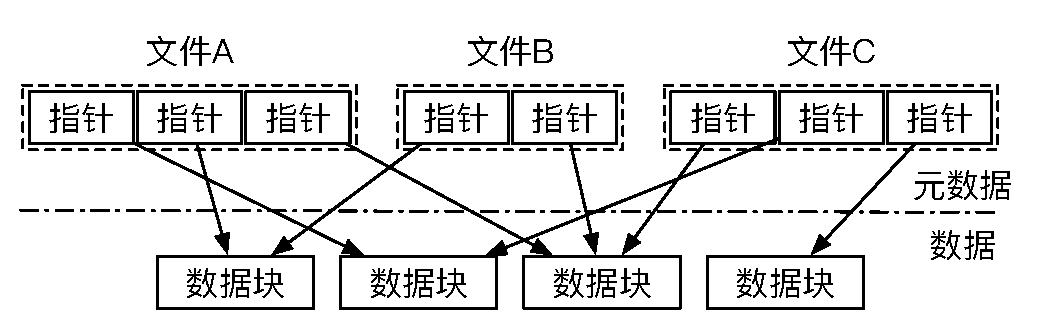
\includegraphics[width=10cm]{DedupSystemStorageMode}
    \caption{数据重删系统的存储模式} 
    \label{fig:数据重删系统的存储模式}
\end{figure}

为了保护数据隐私,加密重复数据删除(encrypted deduplication)增加了一层作用于逻辑数据块的加密操作。如图\ref{fig:加密重复数据删除系统逻辑视图}所示,该加密层基于数据内容来产生加密密钥\citing{bellare2013message}(例如将数据块的哈希值作为密钥\citing{douceur2002reclaiming}),从而将相同的明文数据块加密为相同的密文数据块。系统计算每个密文数据块的哈希值(称为指纹,fingerprint),查询指纹索引(fingerprint index)确定该数据块是否已经存储,最后保存仅具有唯一指纹的密文数据块。需要指出的是,部分加密重复数据删除方案\citing{bellare2013message}采用随机加密算法,但基于明文数据块产生指纹,因此仍然可以通过检查指纹来识别重复数据。

\begin{figure}[!htb]
    \small
    \centering
    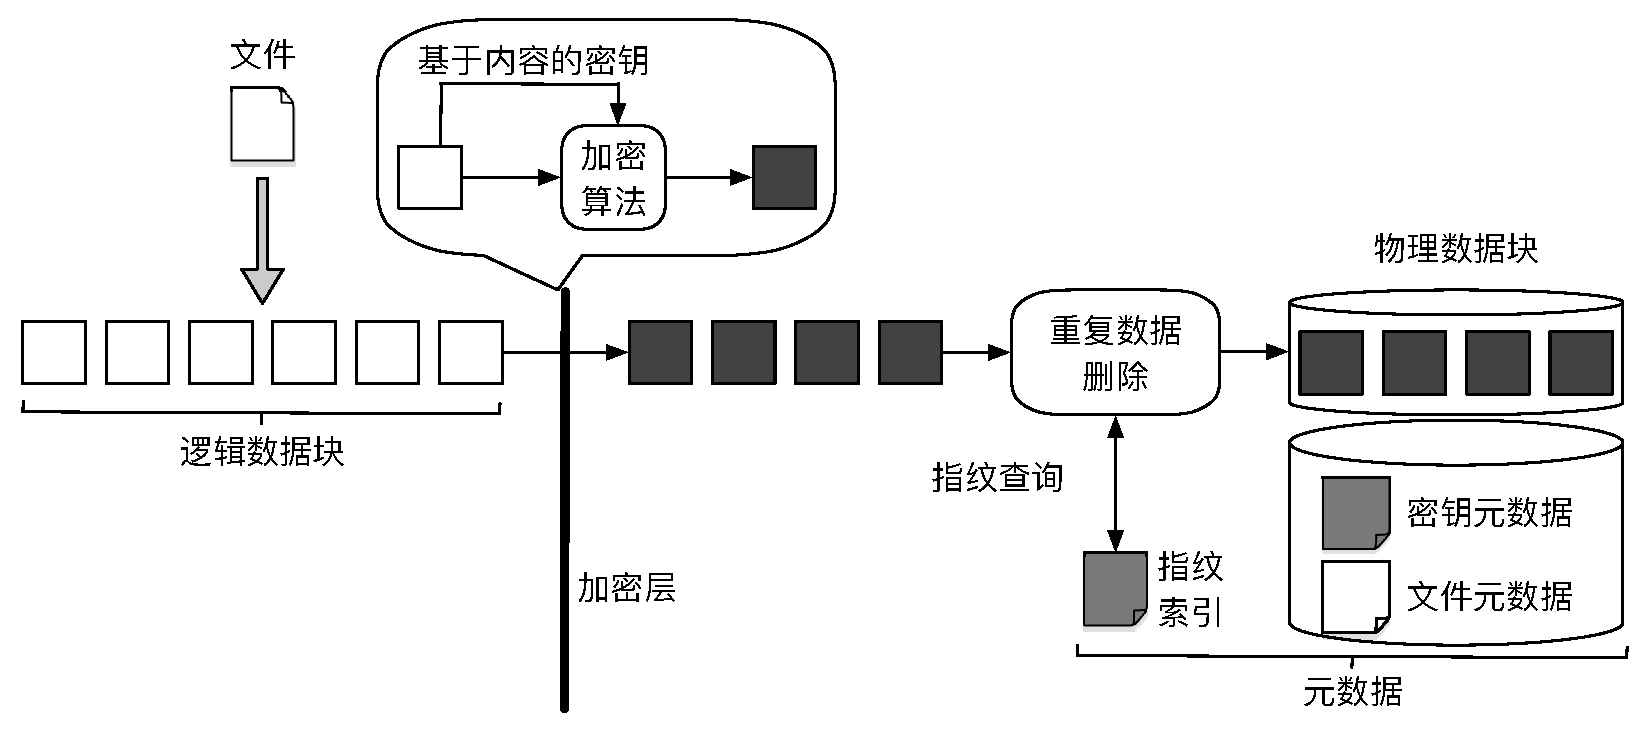
\includegraphics[width=14cm]{EncryptDedupSystemLogic}
    \caption{加密重复数据删除系统逻辑视图}
    \label{fig:加密重复数据删除系统逻辑视图}
\end{figure}

除了指纹索引以外,加密重复数据删除系统须存储额外的元数据(metadata),包括:
\begin{enumerate}
    \item 文件元数据记录了文件内逻辑数据块与相应物理数据块的映射关系,用于重构完整文件。
    \item 密钥元数据记录了文件内逻辑数据块的解密密钥,用于恢复相应的明文内容,由于密钥元数据包含密钥信息,需由文件属主的主密钥(master key)加密后以密文形式存储。
\end{enumerate}

\subsection{问题和动机}

\textbf{密钥生成的安全性和效率平衡问题}

%TODO:数据块信息引用
由于基于数据块内容产生密钥,加密重复数据删除泄漏了数据块的频率信息,即如果一个明文数据块出现了n次,则它对应的密文数据块也将出现n次。另一方面,真实数据集中数据块的出现频率往往呈非均匀分布,调研了FSL和VM备份数据集的数据块频率分布特征,发现三种数据集有超过97\%的数据块的频率低于100次,而至多只有0.04\%的数据块的频率高于10,000次(图\ref{fig:两种真实数据集的数据块频率分布}),这种非均匀的分布特点使攻击者可以利用频率来确定相应数据块。

基于以上原因,认为加密重复数据删除可能受到频率分析\citing{naveed2015inference}的威胁,拟通过本课题,深入研究频率分析攻击对加密重复数据删除安全性的影响,以及提高频率分析攻击效果的方法。

\textbf{重复数据删除中的安全性和效率平衡问题}

从\ S \ ref {sec:introduction}中回想起,现有的加密重复数据删除实现需要昂贵的密码保护。 服务器辅助的MLE必须使用OPRF协议\ cite {naor04}来保护指纹信息免受密钥服务器的侵害,但是OPRF协议涉及昂贵的公钥加密操作(请参见\ S \ ref {subsec:synthetic}中的Exp \#1 )。 同样,当前的PoW实现基于Merkle树协议\ cite {halevi11},该协议对块级PoW执行许多哈希计算。 尽管我们可以通过在每个文件的基础上应用PoW来减轻PoW的计算量(即客户端证明其拥有文件所有权),但是云无法在基于块的重复数据删除下验证块是否属于文件。 现有的提高服务器辅助MLE或PoW性能的解决方案通常会牺牲安全性\ cite {li20b,xu13,pietro12},带宽效率\ cite {harnik10,li15}或存储效率\ cite {zhou15,qin17,li20b}(\ S \ ref {sec:related_work})。


\subsection{研究意义}

本课题研究将填补频率分析攻击研究空白,对理解加密重复数据删除的实际安全性,并降低其在非适合场景下的误用风险具有重要作用。

尽管加密重复数据删除的频率泄漏已是学术界公认的安全问题,但针对性的频率分析攻击研究仍为空白(即利用频率泄漏来获取隐私数据仍是一个开放性问题),致使部分厂商盲目地将加密重复数据删除技术应用于商业产品\citing{MEGA,ElephantDrive}和开源系统\citing{Cryptosphere,Freenet,GNUP2P,Tahoe-LAFS}中。本项目将研究加密重复数据删除技术在频率分析攻击下的实际安全性,以指导其在适合场景下被正确使用。


\section{国内外研究历史与现状}

\subsection{加密重复数据删除}
\label{sec:加密重复数据删除}
在传统对称加密方式下,每个用户具有不同的密钥,不同用户之间的相同明文会被加密为不同密文,难以执行(密文)重复数据删除操作。

消息锁定加密(message-locked encryption,MLE)确立了加密重复数据删除的密码学基础\citing{bellare2013message}:基于数据内容产生密钥(称为 MLE 密钥),从而将相同明文加密为相同密文。最流行的MLE实例是收敛加密(convergent encryption,CE)\citing{douceur2002reclaiming},它使用明文的哈希值作为MLE密钥,并基于密文哈希值计算指纹,以识别重复数据(如图\ref{fig:加密重复数据删除系统逻辑视图})。基于CE的加密重复数据删除方案还包括:

\begin{enumerate}
    \item 哈希收敛加密(hash convergent encryption,HCE)\citing{douceur2002reclaiming}与CE具有相同的MLE密钥产生规则,但基于明文哈希值计算指纹。
    \item 随机收敛加密(random convergent encryption,RCE)\citing{douceur2002reclaiming}使用随机密钥加密以产生非确定的密文,同时也基于明文哈希值来进行重复检查。
    \item 收敛扩散(convergent dispersal,CD)\citing{li2016cdstore}使用明文哈希值作为秘密共享(secret sharing)的输入种子,在兼容重复数据删除的基础上 提高了密文存储的可靠性。
\end{enumerate}

上述MLE实例基于明文产生MLE密钥(CE、HCE和CD)或指纹(HCE和RCE),如果明文是可预测的(即所有可能的明文的数量有限),这些方案易于受到离线暴力破解攻击\citing{bellare2013message,keelveedhi2013dupless}。为了抵御该攻击,DupLESS\citing{keelveedhi2013dupless}基于第三方密钥服务器实现了服务器辅助 MLE(server-aided MLE),确保无法从离线明文派生出相应的MLE密钥。以服务器辅助MLE为基础,现有研究进一步解决了加密重复数据删除的故障容错\citing{li2015cdstore,duan2014distributed}、透明价格模型\citing{armknecht2015transparent}、点对点密钥管理\citing{liu2015secure}、层次密钥管理\citing{zhou2015secdep}等问题。围绕MLE扩展功能的一系列研究包括:兼容加密重复数据删除的数据完整性审计协议\citing{li2016secure};支持动态访问控制的加密重复数据删除系统REED\citing{li2016rekeying,qin2017design}。

无论是MLE还是服务器辅助MLE,均须为相同的明文产生相同的密文(CE、HCE、CD和DupLESS)或指纹(HCE和RCE),泄漏了数据的出现频率。一些理论研究\citing{abadi2013message,stanek2014secure,bellare2015interactive}基于零知识证明、全同态加密、双线性对运算等底层密码技术实现了随机加密,但这些方案存在计算复杂性高、依赖多轮信息交互等问题,难以应用到系统实践中。本文关注可实际应用的加密重复数据删除系统/方案的频率泄漏问题,研究其安全性影响和防御对策。

\subsection{数据所有权证明}
\label{sec:数据所有权证明}

Source-based deduplication is bandwidth-efficient but vulnerable to
side-channel attacks \cite{harnik10} (\S\ref{subsec:encrypted-dedup}). 
Prior studies \cite{harnik10, li15} combine source-based deduplication and
target-based deduplication to defend against side-channel attacks, while
\sysname achieves
significantly more bandwidth savings by purely performing source-based
deduplication (\S\ref{subsec:real-world}) and using PoW to protect against
side-channel attacks.  Also, \sysname is much more efficient than
Merkle-tree-based PoW (\S\ref{subsec:synthetic}).  Some other studies make PoW
efficient by relaxing security (e.g., \cite{pietro12,xu13}), while \sysname
uses client-side SGX to preserve the security of PoW.

\subsection{基于SGX的存储系统}
\label{sec:基于SGX的存储系统}

SGX \cite{sgx} has been widely used for
securing storage systems.  PESOS \cite{krahn18}  enforces the access policies
of object storage with SGX.  OBLIVIATE
\cite{ahmad18} enhances the security of SGX-based file systems against
privileged side-channel attacks. EnclaveDB \cite{priebe18} and ObliDB
\cite{eskandarian19} protect outsourced databases against information leakage
via SGX.  NEXUS \cite{djoko19} enables fine-grained access control with SGX
over untrusted cloud storage.
On the performance side, Harnik {\em et al.} \cite{harnik18} propose
guidelines on mitigating the performance overhead of SGX implementations.
ShieldStore \cite{kim19} implements application-specific
data management to limit the enclave memory usage.  SPEICHER \cite{bailleu19}
is an SGX-based LSM-based key-value store with efficient I/O operations.  

% to address the I/O performance bottleneck
% of enclave.

All the above studies do not consider deduplication. Dang {\em et al.}
\cite{dang17} propose proxy-based protocols for bandwidth-efficient encrypted
deduplication, but the protocols do not address the key generation performance
overhead and have no implementation. SPEED \cite{cui19} leverages deduplication
to make SGX computations efficient, but \sysname improves the performance of
encrypted deduplication with SGX.  SeGShare \cite{fuhry20} maintains a
cloud-side enclave for secure file-based deduplication, while \sysname uses a
client-side enclave to implement an efficient PoW protocol and supports more
fine-grained chunk-based deduplication. 


\section{课题的研究内容、研究目标、以及拟解决的关键问题}
\subsection{研究内容}

% \subsubsection*{加密重复数据删除的频率分析攻击}

% 在传统频率分析模式下,攻击者能够访问明文逻辑数据块集合M和密文逻辑数据块集合$C$($M$和$C$包含重复的明文和密文数据块)。攻击者根据出现频率分别对$M$和$C$中的数据块进行排序,然后将$C$中的密文数据块映射为$M$中与其具有相同排名的明文数据块。但是,传统频率分析在加密重复数据删除中难以形成有效的攻击,主要原因是:$M$和$C$的原始内容可能存在差异(例如$M$和$C$来源于同一个文件系统在不同时间点的备份镜像),将打乱数据块频率排序的对应关系;并且,在频率排序过程中可能存在大量明文和密文数据块具有相同的频率,频率分析难以排序这些数据块来形成正确的对应关系。

% 为了提高传统频率分析的攻击效果,首先研究基于数据特征的新型频率分析攻击技术。然后,分别从抵抗频率排序干扰和降低攻击发生条件两方面改进攻击技术。最后,实现针对真实系统的频率分析攻击原型,并分析该攻击对各类数据安全性的影响。


\subsection{研究目标}

针对以上研究内容,预期实现如下研究目标: 
\begin{enumerate}
    \item 在理论上,设计基于可信计算硬件的密钥生成和数据块所有权证明机制,并在相应安全假设下论证其安全性。
    \item 在技术上,以理论研究为支撑,设计并实现符合安全性假设的低开销的服务器辅助密钥生成和安全且高效的重复数据删除,设并在真实系统中进行理论验证和攻击效果测试。 
\end{enumerate}


\subsection{拟解决的关键问题}

本课题致力于解决传统服务器辅助密钥生成机制和客户端重复数据删除场景下的数据块所有权证明机制的效率问题,难以解决的如下问题:

\begin{enumerate}
    \item How should enclaves be managed?
    \begin{itemize}
        \item Enclave startup incurs high overhead due to remote attestation
        \item Key enclave needs to manage system wide secret information κ
        \item Client machine cannot persistently maintain enclaves
    \end{itemize}
    \item How does key manager prevent online brute force attack?
    \begin{itemize}
        \item Need to enable revocation on clients’ querying key generation oracle
    \end{itemize}
    \item How can key generation performance be further improved?
    \begin{itemize}
        \item Expensive overhead in establishing secure channel (taking ~70\% overallkeygen overhead)
    \end{itemize}
\end{enumerate}


    


    


\section{拟采取的研究方案}
\label{sec:技术路线}



如图\ref{fig:技术路线图}所示,在支撑研究(基于数据块局部性的频率分析攻击方案\citing{li2017information})的基础上,根据相对频率分布特性,设计抗排序干扰的攻击方法;在数据相似性的基础上,设计低依赖条件的攻击方法。最终设计出针对加密重复数据删除方案/系统的新型频率分析攻击方法及对应的原型软件工具。

\begin{figure}[!htb]
    \small
    \centering
    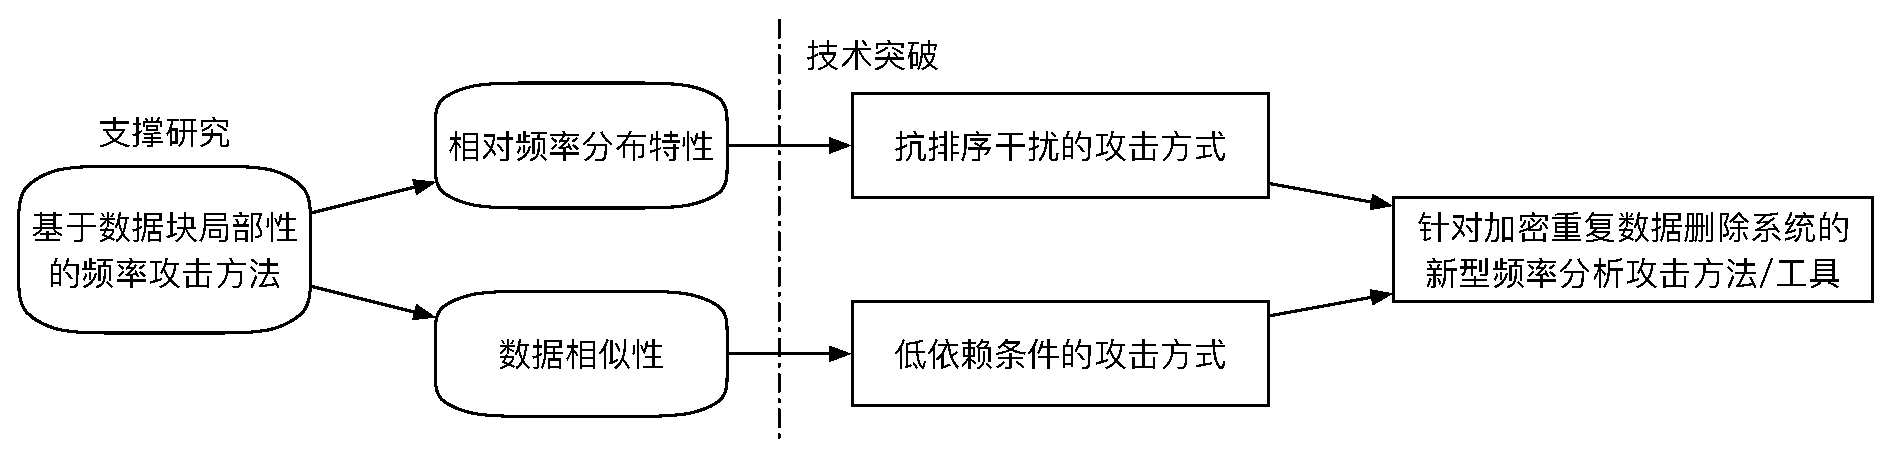
\includegraphics[width=15cm]{TechnicalRoute.eps}
    \caption{技术路线图} 
    \label{fig:技术路线图}
\end{figure}

\subsection{支撑研究}

% 基于数据块局部性的频率分析攻击方案(locality-based attack)\citing{li2017information}作为支撑研究,该方案主要用于破译加密数据备份,即已知的明文数据块集合$M$和目标密文数据块集合$C$源于同一个系统在两个不同时间点的备份镜像。攻击利用了数据块的局部性特征:在不同备份之间,绝大多数数据块保持了相同的局部顺序;例如,每天备份工作项目的进度快照,若一天内的改动较小,则在两次备份之间未被改动的大部分数据块之间的相对顺序保持不变。因此,得出一个关键推论:如果明文数据块M是密文数据块$C$的原始明文,那么M左边和右边相邻的明文数据块有较大可能也是$C$左边和右边相邻密文数据块的原始明文。

% \begin{figure}[!htb]
%     \small
%     \centering
%     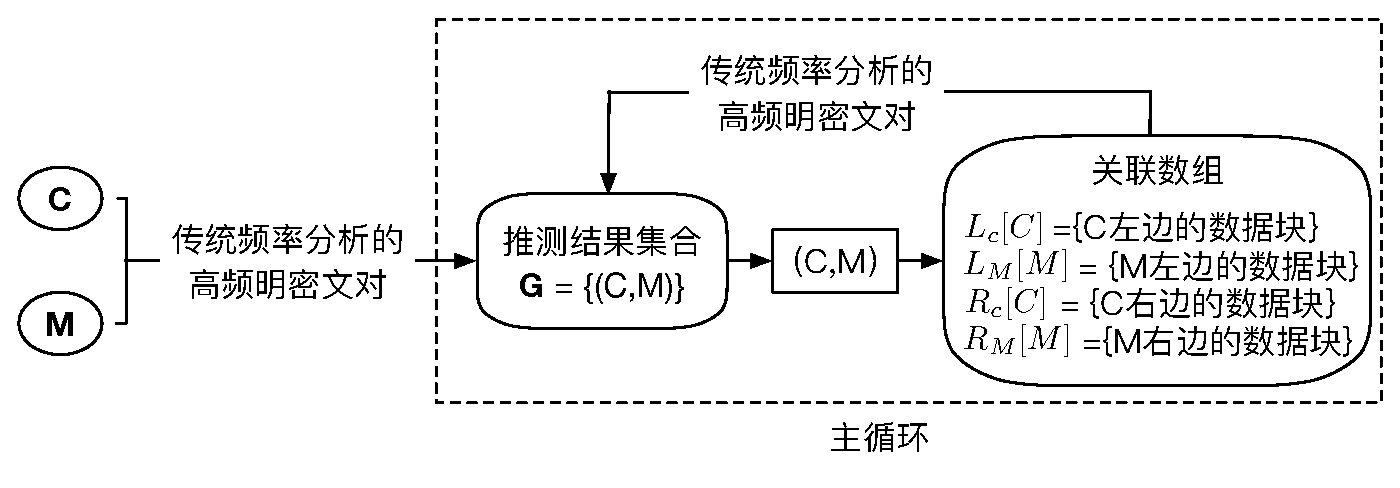
\includegraphics[width=14cm]{BaseFrequencyAttack}
%     \caption{基于数据块局部性的频率分析攻击} 
%     \label{fig:基于数据块局部性的频率分析攻击}
% \end{figure}


% 基于此,攻击流程如图\ref{fig:基于数据块局部性的频率分析攻击}所示:首先,对$C$和$M$应用传统频率分析(\ref{sec:传统频率分析攻击}),将获得的若干组高频明密文对加入推测结果集合 $G$;然后,每次从$G$中选取一组明密文对$(M,C)$,分别对其左右相邻的明文和密文数据块集合$L_M[M]$和$L_C[C]$,以及$R_M[M]$和$R_C[C]$实施频率分析,并将获得的高频明密文对也加入$G$;继续对$G$中的明密文对进行基于相邻数据块的频率分析,直至所有明密文对都被处理。

% 为了验证攻击效果,定义推测率为正确推测出原始明文的(不同)密文数据块个数与$C$中(不同)密文数据块总个数的比率。在基于真实数据集的实验验证中,攻击方案能够达到17.8\%推测率,远远高于传统频率分析方法的0.0001\%推测率。


% \subsection{技术突破}

% \subsubsection{基于分布的频率分析攻击方法}


% \par 基于分布的频率分析攻击利用密文和明文的相对顺序信息来增强频率分析的有效性。该攻击方法建立在数据块局部性\citing{xia2011silo,lillibridge2009sparse,zhu2008avoiding}的基础上。通过以下三个关键特性构造出基于分布的频率分析攻击方法。

% \begin{itemize}
%     \item 数据块局部性指出数据的原始排序可能会在各种备份文件中得以保留,因此可以用于在备份文件中推理出类似的与位置相关的密文-明文对。
%     \item 相邻数据的共现频率的相对频率分布可以通过分析得到。
%     \item 明文及其相应的密文具有相似的相对频率分布的特性。
% \end{itemize}
 
% \subsubsection{基于聚类的频率分析攻击方法}


% 在基于分布的频率分析攻击方法的基础上,通过引入相似性\citing{bhagwat2009extreme}这一属性来消除基于分布的频率分析攻击方法对明文数据的细粒度顺序信息的需求。基于此提出基于聚类的频率分析攻击方法。

\section{可行性分析}

\subsection{研究方法可行}

本课题通过引入加密重复数据删除方案/系统的相关特性来设计新型频率分析攻击方法,针对性提高频率分析攻击方法的有效性。该研究问题具有很高的实际价值且在面向加密重复数据删除的攻击中,已有工作提出了基于数据块局部性(chunk locality)\citing{zhu2008avoiding,lillibridge2009sparse,xia2011silo}的频率分析攻击\citing{li2017information},在此基础上改进攻击方案以提高频率分析攻击实际效果具有明确的可行性。

\subsection{研究条件可行}

前期基于数据块局部性的频率分析攻击方案给出了本课题研究两种新型频率分析攻击方法的基本理论和工具基础。在原有方案上改进即可用于本课题研究。研究者在本科阶段深入钻研了CDStore、REED、SDFS等加密重复数据删除系统,以及前期基于数据块局部性的频率分析攻击方案的理论和工具实现。这些经验可以帮助设计新型频率分析方法以及其在真实系统中的实践。

\section{本研究特色与创新之处}

本研究的特色与创新之处有以下几点:

% \begin{enumerate}
%     \item 研究针对加密重复数据删除提出了两种新型的频率分析攻击方法。除了利用由于加密重复数据删除具有确定性导致的频率泄漏之外,两种攻击都利用重复数据删除工作负载的特性来增加频率分析攻击的有效性。
%     \item 本文研究使用多个真实数据集(包括长期备份\citing{sun2016long,FSL14},Windows文件系统快照\citing{meyer2012study}和VM磁盘映像\citing{li2016cdstore,qin2017design})以及开源重复数据删除系统SDFS\citing{SDFS}、Destor\citing{Destor},评估两种新型频率分析攻击方法和基本频率分析攻击方法的实际效果。通过评估频率攻击方法的攻击结果,进一步分析本频率分析攻击方法对实际加密重复数据删除带来的安全性影响。
%     \item 本研究讨论了减少加密重复数据删除中信息泄漏的可能方案。
% \end{enumerate}

We propose \sysname, a high-performance SGX-based encrypted deduplication
system. \sysname builds on server-aided MLE as in DupLESS \cite{bellare13b},
but executes efficient OPRF-less MLE key generation and PoW inside enclaves.
In particular, it comprises three major building blocks:
%
\begin{itemize}[leftmargin=*] 
\item 
{\em Secure and efficient enclave management}: It protects against the
compromise of the key server and allows a client to quickly bootstrap an
enclave after a restart.
\item 
{\em Renewable blinded key management}: It generates a blinded key for
protecting the communication between the enclave inside the key server and
each of the clients based on key regression \cite{fu06}, such that the blinded
key is renewable for dynamic client authentication. 
\item 
{\em SGX-based speculative encryption}:  It offloads the online
encryption/decryption overhead of an enclave via speculative encryption
\cite{eduardo19}. 
\end{itemize}
\chapter{相关基础研究}
\label{chapter:background}

本章将介绍普通和加密后重复数据删除、可信执行环境(TEE)等本文利用的基础知识,以及加密后重复数据删除系统中存在的性能瓶颈和安全性隐患。

\section{重复数据删除}
\label{sec:background-deduplication}

本文专注于基于数据块的重复数据删除,它以称为数据块的小型数据单元为粒度运行。基于数据块的重复数据删除比基于文件的重复数据删除更精细,因此通常具有更高的存储效率(节省更多的存储空间)。

基于数据块的重复数据删除有以下两种基本的数据块分块方法:

\begin{itemize}[leftmargin=*]
    \item \textbf{固定大小的数据分块(Fixed-size chunking)},通常将文件划分为固定长度的数据块,具有简单快速的特点,但文件中小范围修改(例如:增加1字节内容或删除1字节内容)将从修改位置开始影响后续所有数据块的内容,不利于重复数据删除。
    \item \textbf{可变大小的数据分块(Variable-size chunking)},也称为内容定义的数据块分块(Content-defined chunking)。通常采用内容相关的方式指定数据块的边界(例如,通过Rabin指纹\cite{rabin1981fingerprinting}在特定内容模式出现时进行分块)。因此,在文件发生小范围修改时,产生的大多数数据块仍可保持不变,使得重复数据删除系统存储效率得到保障。
\end{itemize}

在多数备份系统工作负载\cite{zhu2008avoiding,lillibridge2009sparse}下,可变大小的数据分块方案通常可以获得更优的存储效率,但在某些特定工作负载(例如,VM备份数据集\cite{jin2009effectiveness})下,固定大小的数据分块方案却更加有效。本文的工作可兼容固定大小和可变大小的数据分块方法产生的数据块。

\begin{figure}[!htb]
    \small
    \centering
    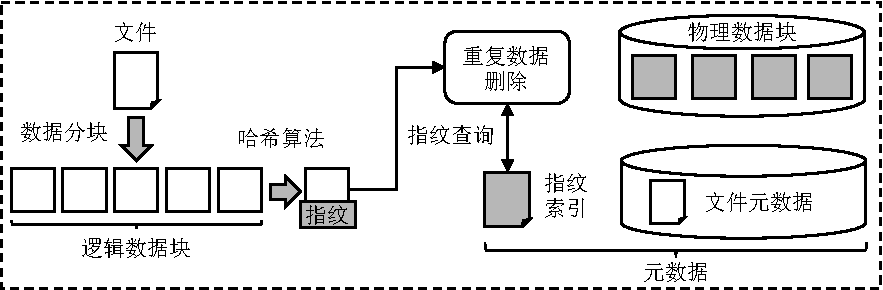
\includegraphics[width=\textwidth]{chunk-based-dedup-arch.pdf}
    \caption{基于数据块的重复数据删除的工作流程概览}
    \label{fig:chunk-based-dedup-flow}
\end{figure}

图\ref{fig:chunk-based-dedup-flow}总结了基于数据块的重复数据删除工作流程。具体地,重复数据删除系统首先通过数据分块过程将客户端的文件(例如,备份文件)分割为逻辑数据块,根据每一个逻辑数据块的内容,使用哈希算法计算得到其对应的唯一标签(又称为指纹)。如果两个数据块具有相同的指纹,则认为两个数据块内容相同(不同逻辑数据块计算得到相同指纹的概率可忽略不计\cite{black2006compare});若两个逻辑数据块指纹不一致,则认为两逻辑数据块不同。重复数据删除系统仅存储相同逻辑数据块的唯一副本(称为物理数据块),并且每个相同的逻辑数据块仅通过一个空间开销较小的索引指向相同的物理数据块。此外,基于数据块的重复数据删除系统记录文件所拥有的所有逻辑数据块的信息作为该文件的元数据,用于文件读取、删除等操作。

重复数据删除技术根据重复数据删除操作发生的位置可分为源端重复数据删除及目标端重复数据删除\cite{IDC2010Data}:

\begin{itemize}[leftmargin=*]
    \item \textbf{源端重复数据删除(Source-based Deduplication)}由客户端计算目标数据块的哈希值,并由服务端检查该哈希值是否存在于索引表中。如果哈希值存在(即服务端已有目标数据块的副本),则通知客户端无需传输目标数据块。
    \item \textbf{目标端重复数据删除(Target-based Deduplication)}强制客户端传输所有密文数据块,并在服务端对所有收到的密文数据块进行重复数据删除。
\end{itemize}

源端重复数据删除技术可有效节省网络流量资源,可显著降低云服务商提供存储服务的成本,但泄露了“其他客户端是否已经存储相应密文数据块”的侧信道信息(参见\S\ref{subsubsec:intro-problem-security});目标端重复数据删除具有更高的隐私保护能力,但产生大量网络资源浪费,并显著增加了服务端计算开销。本文关注网络资源开销较小的源端重复数据删除技术,并通过TEE技术解决其存在的性能和安全性问题。

\section{安全重复数据删除}
\label{sec:background-enc-deduplication}

加密后重复数据删除解决了外包环境(例如,云存储)中的数据块机密性保障问题,同时保持了重复数据删除的有效性。出于安全因素考虑,用户希望将自己的数据加密后再进行外包存储,以确保个人数据隐私性。传统对称加密算法算法为每个客户端或每个逻辑数据块分配独立的加密密钥,使得来自不同(或相同)客户端的相同的逻辑数据块被加密为不同的密文数据块,服务器无法感知这些密文数据块所对应的明文数据块内容是否一致,使得针对外包数据的重复数据删除完全失效。

\begin{figure}[!htb]
    \small
    \centering
    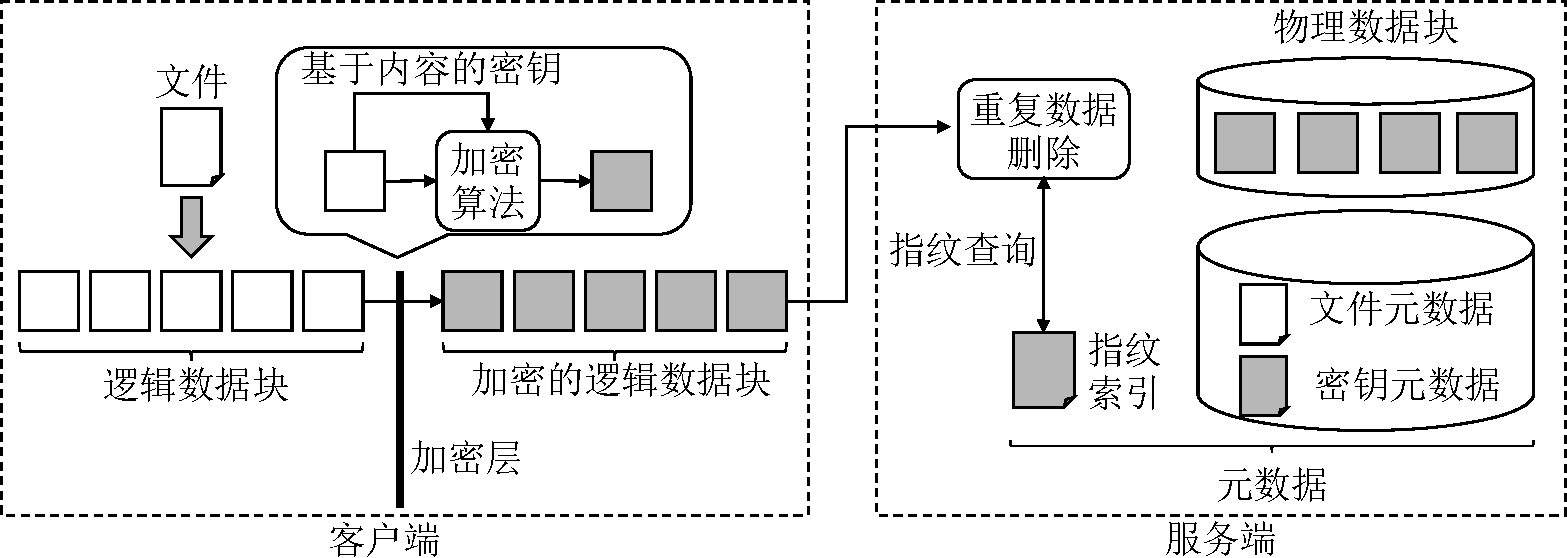
\includegraphics[width=\textwidth]{chunk-based-enc-dedup-arch.pdf}
    \caption{基于数据块的加密后重复数据删除的工作流程概览}
    \label{fig:chunk-based-enc-dedup-flow}
\end{figure}

如图~\ref{fig:chunk-based-enc-dedup-flow}所示,基于内容的密钥生成方法给加密后重复数据删除提供了新的处理思路。最基本的基于内容的密钥生成方法的实例化是基于明文数据的内容(例如,基于重复数据删除中的逻辑数据块)导出其对称加密密钥,并使用该密钥加密明文数据以形成对应的密文数据(例如,加密的逻辑数据块)。因此,使用基于内容的密钥生成方法为任意逻辑数据块产生对称加密密钥可以确保将相同的明文数据块加密为相同的密文数据块。最后,存储系统从每个密文数据块中导出其对应的指纹并执行重复数据删除。相较于普通重复数据删除,加密后重复数据删除需额外保存用户文件所包含数据块的密钥元数据,并由各个客户端进行加密以防止服务端取得相应数据块的明文内容。

\subsection{数据块加密技术}
\label{subsec:background-encrypted-deduplication-key}

\textit{消息锁加密(Message-Locked Encryption, MLE)}\cite{bellare2013MLE}将基于内容的密钥生成方案等加密原语形式化用于加密后重复数据删除。它指出了如何从明文数据块的内容导出相应的对称加密密钥(称为 \textit{消息锁加密密钥(MLE密钥)})。以最广泛使用的消息锁加密技术:收敛加密(Convergent Encryption, CE)\cite{douceur2002reclaiming}为例,CE使用明文数据块的安全哈希作为MLE密钥,使得相同的明文数据块可被加密为相同的密文数据块,从而令重复数据删除技术在密文数据块之上仍然可行。除此之外,基于CE的消息锁加密方案还包括:

\begin{enumerate}[leftmargin=*]
    \item \textbf{哈希收敛加密(Hash Convergent Encryption, HCE)}\cite{douceur2002reclaiming}与CE具有相同的MLE密钥产生规则,但基于明文哈希值计算指纹用于重复数据删除(CE使用密文指纹进行重复数据删除)。
    \item \textbf{随机收敛加密(Random Convergent Encryption, RCE)}\cite{douceur2002reclaiming}使用随机密钥加密明文以产生非确定的密文,但基于明文的哈希值进行重复数据删除检查。
    \item \textbf{收敛扩散(Convergent Dispersa, CD)}\cite{li2016cdstore}使用明文哈希值作为秘密共享(Secret Sharing)的输入种子,并对产生的多个秘密共享分别计算哈希并进行重复数据删除,在兼容重复数据删除的基础上提高了密文存储的可靠性。
\end{enumerate}

然而,CE容易受到\textbf{离线暴力破解攻击}的威胁。这是由于CE的MLE密钥(即明文数据块的哈希)可以自由产生。具体来说,攻击者通过枚举所有可能的明文数据块的MLE密钥来从目标密文数据块(其加密密钥未知)推断输入的明文数据块,以检查是存在某个明文数据块被加密到目标密文数据块。

服务器辅助消息锁加密(Server-aided MLE)\cite{bellare2013DupLESS}是最先进的加密原语,可增强加密后重复数据删除对离线暴力攻击的安全性。它为消息锁加密中的MLE密钥生成步骤部署了一个专用的\textbf{密钥服务器(key server)}。为了加密明文数据块,客户端首先将明文数据块的指纹发送到密钥服务器,密钥服务器通过指纹和密钥服务器维护的\textbf{全局秘密(global secret)}返回MLE密钥。如果全局秘密是安全的,则攻击者无法发起离线暴力攻击;如果全局秘密被泄露,则其安全性会降低到原始消息锁加密的安全性。服务器辅助消息锁加密建立在如下两种安全机制之上:

\begin{itemize}[leftmargin=*]
    \item \textbf{遗忘伪随机函数(oblivious pseudorandom function, OPRF)}\cite{naor2004Number}是一种安全计算协议,协议包含服务端和客户端,服务端持有密钥$k$,客户端持有输入$x$,双方通过交互来联合计算函数$f_k(x)$,最终由客户端得到函数值。OPRF的计算过程以盲化方式进行,即在计算过程中服务端无法获取关于$x$的任何有价值信息,同时客户端无法获取关于$k$的任何有价值信息。
    \item \textbf{速率限制(Rate-limiting)}\cite{bellare2013DupLESS}阻止特定操作频率超出某些限制。在大型系统中,速率限制通常用于保护底层服务和资源。
\end{itemize}

基于遗忘为随机函数,密钥服务器可依据客户端发送明文数据块的“盲化指纹”,进而基于盲指纹和全局秘密产生对应数据块的“盲化密钥”,阻止了密钥服务器了解明文数据块信息;并使得客户端可在不了解密钥服务器所拥有的全局秘密的条件下获得目标明文数据块的MLE密钥。对来自客户端的密钥生成请求进行速率限制,进一步防止恶意客户端向密钥服务器发出海量密钥生成请求以获得目标MLE密钥,限制了攻击者暴力破解攻击的速度。

\subsection{数据所有权证明技术}
\label{subsec:background-encrypted-deduplication-pow}

为了节省宝贵的网络带宽资源,现有加密后重复数据删除系统普遍采用源端重复数据删除,以便在客户端删除重复数据块,而无需上传到服务端(\S\ref{sec:background-deduplication})。但是,源端重复数据删除导致“目标数据块是否已在服务端存储”的侧信道信息,使得某些客户端存在恶意时,源端重复数据删除很容易受到侧信道攻击(\textit{Side-channel Attack})\cite{harnik2010side,halevi11}的影响。

一种典型的侧信道攻击被称为\textbf{伪造所有权攻击}:恶意客户端未授权访问其他客户端存储的数据块\cite{harnik2010side,mulazzani11}。具体来说,由于服务端仅能基于收到的数据块哈希值判断客户端是否拥有对应的数据块,攻击者可使用任意目标密文数据块的指纹来说服服务端其是该目标数据块的所有者,进而获得该数据块的完全访问权限(\S\ref{subsec:intro-background});另一种侧信道攻击被称为\textbf{推测内容攻击}:恶意客户端将目标密文数据块指纹发送到服务端以检查该数据块是否存在(例如,目标密文数据块对应于某个可能的密码\cite{harnik2010side}),以此识别来自其他客户端的敏感信息(\S\ref{subsubsec:intro-problem-security})。

现有防御机制尚无法在执行源端重复数据删除且不大量增加额外网络带宽资源开销的前提是防御推测内容攻击。而为了防止伪造所有权攻击,源端加密后重复数据删除增加了所有权证明(proof-of-ownership, PoW)机制\cite{halevi11},要求客户端额外向服务端提交目标密文数据块的所有权证明(proof),且仅在所有权证明成功的条件下进行重复数据删除。所有权证明机制可使得服务端只针对客户端真实拥有(即具有完整访问权限)的密文数据块执行重复数据删除,避免了攻击者非法访问其他客户端已在云服务端存储的内容。现有基于默克尔树(Merkel Tree)的所有权证明机制(称为POW-MT)\cite{xu2013weak}使用纠删码对数据块进行编码,随后在纠删码编码结果的基础上建立默克尔树用于所有权证明。而另一种基于通用哈希函数(Universal Hash)的所有权证明机制(称为POW-UH)\cite{halevi2011proofs} 相较于基于默克尔树的所有权证明机制拥有更高的效率,但降低了安全性假设。

本文关注网络和服务端计算资源开销较小的源端重复数据删除技术,并通过TEE技术解决其存在的密钥生成和所有权证明效率问题,以及易受到推测内容攻击的安全性问题。

\section{可信执行环境(TEE)}
\label{sec:background-tee}

TEE全名为可信执行环境(Trusted Execution Environment)是计算平台上由软件协同硬件方法构建的一个安全区域,可以确保在安全区域内加载的程序和数据在完整性和机密性方面得到必要保护。其目标是确保目标程序按照预期执行,保证程序初始状态和运行时状态的机密性、完整性。针对TEE的相关概念及规范定义,各个软件、硬件厂商结合自己的基础架构形态产生的具体实现各不相同。虽然在技术实现上存在显著差异,但TEE的技术共同点可总结为如下三点:

\begin{itemize}[leftmargin=*]
    \item \textbf{隔离性}:
          TEE通过隔离的程序执行环境,提供一个可信的执行空间,为其中运行的程序和存储的数据提供了机密性和完整性保护。X86架构的隔离机制从Intel 80286处理器开始,Intel提出了CPU的两种运行模式,并且逐步衍生出后来的不同的特权界别,再后来提出了安全区域范围更小的SGX机制实现可信执行环境(TEE);同样的,ARM架构通过TrustZone技术实现了相关软硬件的隔离性,实现了安全世界(Secure World)与非安全世界(Normal World)的隔离。
    \item \textbf{软硬协同性}:
          虽然标准定义可以通过单独软件方式或单独硬件方式实现TEE,但实际应用场景下,行业内更多选择通过软硬件结合的方式进行TEE的设计。
    \item \textbf{富表达性}:
          与传统安全新芯片或纯软件的密码学营私保护方案相比,TEE支持的上层业务表达性更强,软件开发者仅需要根据业务逻辑划分业务层面的隐私和非隐私区域,而不会对定义隐私区域内的算法逻辑的语言等有可计算性方面的限制(图灵完备的)。同时,由于TEE为程序提供了可信的执行环境,安全区内的数据无需进行密态运算,使得TEE应用可以支持更多的算计及复杂的算法。
\end{itemize}

\subsection{Intel SGX}
\label{subsec:background-tee-sgx}

\begin{figure}[!htb]
    \small
    \centering
    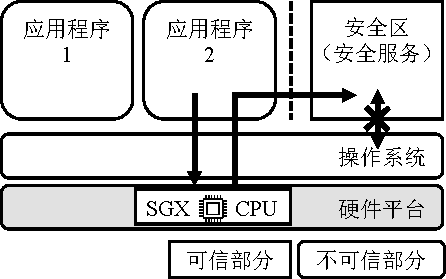
\includegraphics[width=0.6\textwidth]{sgx-example.pdf}
    \caption{Intel SGX框架}
    \label{fig:sgx-arch}
\end{figure}

Intel Software Guard Extensions (Intel SGX)\cite{sgx,sgx2},是一组内置于现代Intel CPU中用于增强应用程序代码和数据安全性的扩展指令。开发者可利用SGX技术将应用程序的安全操作封装在称为“安全区(Enclave)”的硬件保护环境中,保障用户关键代码和数据的机密性和完整性。Intel SGX最关键的优势在于将应用程序以外的软件栈如操作系统(OS)和基本输入输出系统(BIOS)都排除在了可信计算基(Trusted Computing Base, TCB)之外,一旦程序和数据在安全区之中,即便是操作系统和也无法影响安全区内的代码和数据,安全区的安全边界只包含CPU和它本身(如图\ref{fig:sgx-arch}所示)。Intel SGX具有隔离、证明和密封三项主要安全功能。

\textbf{隔离(Isolation)}:安全区代码和数据被放置在被称为\textit{enclave page cache (EPC)}的硬件内存保护区域中,该内存区域使用内存加密引擎(MEE)进行加密,以防止泄露任何内存数据到本安全区之外。EPC以大小为4\,KiB的页面为基本单位管理安全区内存,任意安全区内应用程序最多可占用96\,MiB内存空间\cite{harnik2018SGX}。当安全区内存使用超过上限时,须将未使用的内存页面加密并逐出到未受保护的主存,并在将逐出的页面加载回安全区内存时解密并验证完整性,导致巨大的分页开销\cite{arnautov2016SCONE,dinhngoc2019Everything}。

此外,SGX为安全区和未受保护的内存之间的交互提供了两个接口,应用程序可以通过安全区内部调用(ECalls)进入安全区以执行安全区内部函数,并且在ECall中,程序可通过安全区外部调用(OCalls)暂时退出安全区并调用不受保护的内存中的不受信任的函数。但安全区内部调用和外部调用会产生大量的CPU上下文切换开销\cite{harnik2018SGX},严重影响SGX应用程序性能。

\textbf{认证(Attestation)}:SGX安全区支持本地认证(Local Attestation)和远程认证(Remote Attestation),以确保安全区内运行的程序未被修改。特别的,在远程认证过程(参见\cite{SGX-RA}提供的端到端远程认证示例)中,远程实体(例如,服务端)需要联系Intel运营的证明服务来检查目标安全区提供的安全区相关信息的完整性和正确性。随后,远程实体通过将其收到的安全区信息与目标安全区中预期的可信信息进行比较来验证目标安全区是否未被修改。然而,由于远程认证需要Intel服务器的支持,远程认证过程通常导致较高且不可控的时间开销。

\textbf{密封(Sealing)}: SGX安全区通过密封在安全区内容需要在安全区外持久化存储时进行保护。它使用目标安全区专用的密封密钥(Sealing key)在数据被移出安全区之前进行加密。密封密钥可以从安全区测量哈希(Measurement hash,即安全区内容的SHA-256哈希)或安全区的创建者提供的签名身份派生。基于前者产生的密封密钥仅有目标安全区本身可以导出,而基于后者产生的密封密钥可有同一开发者创建的各个不同的安全区导出。因此,仅有相应的安全区才能获得正确的密封密钥并解密密封数据。

\subsection{ARM TrustZone}
\label{subsec:background-tee-tz}

ARM TrustZone\cite{trustzone}是ARM公司为Cortex-A微架构\cite{cortex-a}设计的一种TEE解决方案,其目的是为其产品构建一个安全框架来抵御各种可能的攻击,它通过对原有硬件架构进行修改,在处理器层次引入了两个不同权限的保护域:安全世界(Secure World)和非安全世界(Normal World),并防止运行于非安全世界的软件直接访问安全世界资源。

如图~\ref{fig:ARM-TZ-base}(a)所示,ARM引入了一种称为监视模式的处理器模式,该模式负责在世界过渡时保留处理器状态,两个世界可以通过称为安全监视器调用(Secure Monitor Call, SMC)的特权指令进入监视模式并实现彼此切换。

\begin{figure}[!htb]
    \small
    \centering
    \begin{tabular}{@{}c@{}c@{}c}
        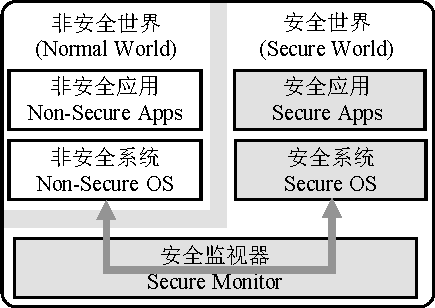
\includegraphics[width=0.49\textwidth]{ARM-TZ-A.pdf} &
        \hspace{5pt}
        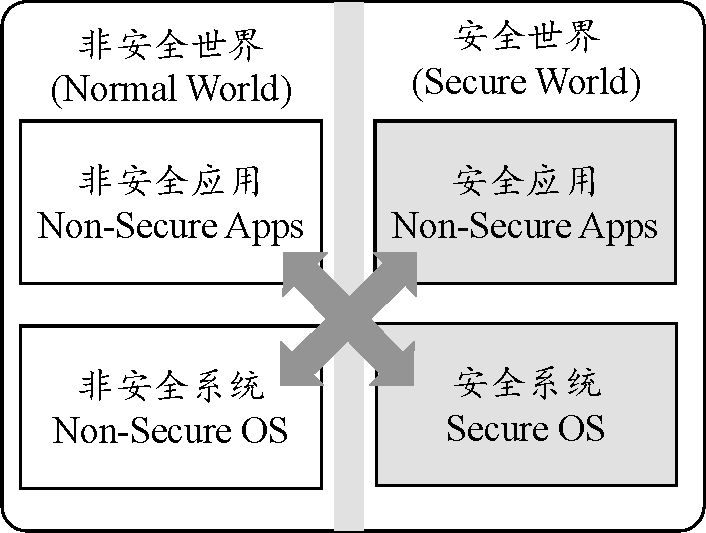
\includegraphics[width=0.49\textwidth]{ARM-TZ-M.pdf}   \\
        \mbox{\small (a) Cortex-A微架构中的TrustZone}        &
        \mbox{\small (b) Cortex-M微架构中的TrustZone}          \\
    \end{tabular}
    \caption{ARM TrustZone技术}
    \label{fig:ARM-TZ-base}
\end{figure}

除了Cortex-A微架构外,ARM发布的新一代Cortex-M微架构\cite{cortex-m}同样为TrustZone提供了硬件支持。与Cortex-A相同的是,Cortex-M依旧将处理器运行状态划分为安全世界和非安全世界,并阻止运行于非安全世界的软件直接访问安全资源。不同的是,Cortex-M针对更快的上下文切换和低功耗应用进行了优化。具体来说,Cortex-M中世界之间的划分是基于内存映射的,并且转换是在异常处理代码中自动发生的(如图~\ref{fig:ARM-TZ-base}(b)所示)。这意味着,当从安全内存运行代码时,处理器处于安全世界,而当从非安全内存运行代码时,处理器处于非安全世界。Cortex-M中的TrustZone技术排除了监视模式,也不需要任何安全的监视软件,这大大减少了安全世界与非安全世界的切换延迟,使得世界之间的转换为更高效。

各芯片产商根据ARM公司对于TrustZone的硬件设计在各自具体的芯片上进行设计和实现,基于TrustZone技术,可以搭建一个可信执行环境(TEE),并在TEE内运行基于TrustZone的操作系统,如高通的QSEE、开源的OP-TEE等。

\section{本章小结}

本章介绍了普通与加密重复数据删除,现有加密重复数据删除中数据块加密技术和数据所有权证明技术导致的性能问题,以及可信执行环境的相关内容。

\chapter{基于可信执行环境(TEE)加速加密后重复数据删除}
\label{chapter:sgxdedup}

\section{简介}
\label{sec:sgxdedup-introduction}

将数据存储管理外包到云端是客户(企业或个人)节省自行管理海量数据开销的常用方案,\textit{安全性}和\textit{存储效率} 是实际外包存储的两大目标。为了满足这两个目标,我们探索了 \textit{(加密后重复数据删除(encrypted deduplication)},这是一种通过始终将重复的明文数据块(来自相同或不同的客户端)加密为重复的密文数据块,并使用从块内容本身派生的密钥来结合加密和重复数据删除的范例;例如,密钥可以是相应块 \cite{douceur02} 的加密哈希。因此,可以通过重复数据删除来消除任何重复的密文数据块以提高存储效率,同时对所有外包块进行加密以防止未经授权的访问。加密后重复数据删除特别适用于备份应用程序,这些应用程序具有高内容冗余 \cite{wallace12} 并且是外包存储 \cite{hasan05,kotla07,varble09} 的有吸引力的用例。
  
现有的加密后重复数据删除方法通常会产生很高的性能开销来实现安全保证。我们使用最先进的加密后重复数据删除系统 {\em DupLESS} \cite{bellare13b} 作为代表性示例来解释性能问题(详见\S\ref{subsec:sgxdedup-encrypted-dedup})。首先,为了防止对手推断出内容派生的密钥,{\em DupLESS} 采用了 \textit{服务器辅助密钥管理(server-aided key management)},其中部署了一个专用的密钥管理器来管理来自客户端的密钥生成请求。但是,服务器辅助密钥管理需要昂贵的加密操作,以防止密钥管理器在密钥生成期间知道明文数据块和密钥。其次,为了防止对手通过推断重复数据删除模式(又名旁道攻击\cite{harnik2010side, halevi2011proofs})获得对密文数据块的未经授权的访问,{\em DupLESS} 可以采用以下方法之一: (i)执行 \textit{基于存储目标的重复数据删除}(即上传所有密文数据块并让云删除任何重复的密文数据块)以便保护重复数据删除模式免受任何(恶意)客户端的影响,或(ii)执行\textit{源端重复数据删除}(即,删除客户端上所有重复的密文数据块而不上传到云),另外向云证明它确实是密文数据块的所有者(即,可以访问相应明文数据块的全部内容)和被授权对密文数据块执行重复数据删除。前者需要额外的通信带宽来上传重复的密文数据块,而后者需要昂贵的密码操作来证明客户端是密文数据块的所有者。尽管已经提出了各种协议设计来解决加密后重复数据删除的性能问题,但它们往往会削弱安全性 \cite{li20b,xu13,pietro12},增加带宽开销 \cite{harnik10,li15},或降低存储效率 \cite{zhou15, qin17,li20b}(详见 \S\ref{sec:sgxdedup-related_work})。
  
硬件辅助可信执行 \cite{trustzone,sgx,Mktem,Amdsev} 的进步为提高加密后重复数据删除的性能提供了新的机会。特别是,我们专注于Intel软件保护扩展 (SGX),它提供了一个 \textit{ 可信执行环境 (TEE)},称为 \textit{ enclave},用于处理具有机密性和完整性保证的代码和数据 \cite{baumann14 }。鉴于 SGX 通过适当的配置 \cite{harnik18} 实现了相当高的性能,我们有动力通过直接在安全区中运行敏感操作来卸载加密后重复数据删除的昂贵加密操作,从而提高加密后重复数据删除的性能,同时保持其安全性、带宽效率和存储效率。

我们提出了 \sysnameS,这是一个基于 SGX 的高性能加密后重复数据删除系统。 \sysnameS 建立在 {\em DupLESS} \cite{bellare13b} 中的服务器辅助密钥管理之上,但在安全区内执行高效的加密操作。实现 \sysnameS 的设计具有不小的挑战。首先,安全地引导安全区以托管受信任的代码和数据至关重要,但证明安全区的真实性会导致显着延迟。其次,每个客户端都需要通过安全通道与密钥管理器内部的安全区进行通信,但安全通道的管理开销会随着客户端数量的增加而增加。最后,客户端可以续订或撤销云服务订阅,因此允许动态客户端身份验证至关重要。为此,我们为 \sysnameS 实现了三个主要构建块: 

\begin{itemize}[leftmargin=*]
    \item \textit{安全高效的安全区管理}:
        它可以防止密钥管理器受到破坏,并允许客户端在重新启动后快速引导安全区。
    \item \textit{自更新盲密钥管理}:
        它基于密钥回归 \cite{fu06} 生成一个盲密钥,用于保护密钥管理器内的安全区和每个客户端之间的通信,以便可以更新盲密钥以进行动态客户端身份验证。
    \item \textit{基于 Intel SGX的推测性加密}:
        它通过推测性加密 \cite{eduardo19} 减轻了安全通道管理的在线加密/解密开销。
\end{itemize}

我们使用合成和真实的 \cite{fsl,meyer11} 工作负载来评估我们的 \sysnameS 原型。它通过将加密操作卸载到安全区来实现显着的加速(例如,与 {\em DupLESS} \cite{bellare13b} 中的原始密钥生成方案相比,密钥生成加速了 131.9$\times$,在 Merkle-tree 上计算 PoW 加速了 8.2$\times$ -基于 PoW \cite{halevi11})。对于非重复和重复数据的上传,它还分别比 {\em DupLESS} \cite{bellare13b} 实现了 8.1$\times$ 和 9.6$\times$ 的加速,并且在实际中节省了高达 99.2\% 的带宽/存储 -世界工作量。我们在 {\bf http://adslab.cse.cuhk.edu.hk/software/sgxdedup} 上发布了我们的 \sysnameS 原型的源代码。 


\section{背景和问题}
\label{sec:sgxdedup-background}

我们介绍了加密后重复数据删除 (\S\ref{subsec:sgxdedup-encrypted-dedup}) 和Intel SGX (\S\ref{subsec:sgxdedup-sgx}) 的背景细节和正式定义。我们还介绍了本文中提到的威胁模型 (\S\ref{subsec:sgxdedup-threat})。

\subsection{加密后重复数据删除}
\label{subsec:sgxdedup-encrypted-dedup}

{\bf } 我们考虑\textit{基于数据块的重复数据删除} \cite{zhu2008avoiding,wallace12,meyer11},它广泛部署在现代存储系统中以消除内容冗余。它通过将输入文件划分为不重叠的 \textit{数据块} 来工作。对于每个块,它计算块内容的加密哈希(称为 \textit{指纹})。它在\textit{指纹索引} 中跟踪所有当前存储的块的指纹。如果指纹是指纹索引的新指纹,它只存储块的物理副本,或者如果指纹已被跟踪,则将块视为副本,假设指纹冲突在实践中极不可能 \cite{black2006compare}。
   
加密后重复数据删除通过加密扩展了基于数据块的重复数据删除,为外包云存储提供数据机密性和存储效率。 \textit{ 客户端} 使用一些对称密钥将输入文件的每个 \textit{ 明文数据块} 加密成一个 \textit{ 密文数据块},并将所有密文数据块存储在 \textit{ 云}(或任何远程存储站点)中,它管理密文数据块的重复数据删除存储。为了支持文件重建,客户端创建了一个 \textit{ file recipe},其中列出了密文数据块的指纹、大小和密钥。它使用自己的主密钥加密文件元数据,并将加密的文件元数据存储在云中。

\textit{ 消息锁定加密 (消息锁加密(MLE))} \cite{bellare2013MLE} 将加密原语形式化用于加密后重复数据删除。它指定了对称密钥(称为 \textit{ 消息锁加密(MLE) 密钥})如何从明文数据块的 \textit{ content}(例如,其流行的实例化 \textit{ convergent encryption (CE)} \cite{douceur02}使用明文数据块的加密哈希作为 消息锁加密(MLE) 密钥)。因此,它将重复的明文数据块加密为重复的密文数据块,从而使重复数据删除在密文数据块上仍然可行。

\paragraph*{Server-aided 消息锁加密(MLE).} CE 易受 \textit{ 离线暴力攻击},因为它的 消息锁加密(MLE) 密钥(即明文数据块的哈希)可以公开派生。具体来说,攻击者通过枚举所有可能的明文数据块的 消息锁加密(MLE) 密钥来从目标密文数据块(不知道 消息锁加密(MLE) 密钥)推断输入明文数据块,以检查是否有任何明文数据块被加密到目标密文数据块。

服务器辅助消息锁加密(Server-aided MLE)\cite{bellare2013DupLESS} 是最先进的加密原语,可增强加密后重复数据删除对离线暴力攻击的安全性。

它为消息锁加密(MLE) 中的密钥生成步骤部署了一个专用的 \textit{ 密钥管理器(key server)}。为了加密明文数据块,客户端首先将明文数据块的指纹发送到密钥管理器,密钥管理器通过指纹和密钥管理器维护的\textit{ global secret}返回 消息锁加密(MLE) 密钥。如果全局机密是安全的,则对手无法发起离线暴力攻击;否则,如果全局机密被泄露,则安全性会降低到原始 消息锁加密(MLE) 的安全性。服务器辅助 消息锁加密(MLE) 进一步建立在两种安全机制之上。首先,它使用 \textit{ oblivious pseudorandom function (OPRF)} \cite{naor04} 允许客户端发送明文数据块的“盲”指纹,这样密钥管理器仍然可以返回相同的 消息锁加密(MLE) 密钥用于相同指纹无需学习原始指纹。其次,它对来自客户端的密钥生成请求进行速率限制,以防止恶意客户端向密钥管理器发出许多密钥生成请求,以找到目标 消息锁加密(MLE) 密钥。

\paragraph*{Proof-of-ownership.} 为了节省带宽,加密后重复数据删除可以应用源端重复数据删除,而不是基于存储目标的重复数据删除,以在客户端删除重复的密文数据块,而无需上传到云(\S\ref{sec:sgxdedup-introduction})。客户端将密文数据块的指纹发送到云端,云端检查指纹是否被指纹索引跟踪(即对应的密文数据块已被存储)。然后,客户端仅将非重复密文数据块上传到云端。


但是,当某些客户端受到威胁时,源端重复数据删除很容易受到 \textit{ side-channel attack} \cite{harnik10,halevi11} 的攻击。一种侧信道攻击是,受感染的客户端可以通过将密文数据块的指纹发送到云来查询任何目标密文数据块的存在(例如,如果密文数据块对应于某个可能的密码 \cite{harnik10}),因此以识别来自其​​他客户端的敏感信息。另一种侧信道攻击是受感染的客户端可以未经授权访问其他客户端的存储块。具体来说,它可以使用任何目标密文数据块的指纹来说服云它是具有完全访问权限 \cite{halevi11} 的相应密文数据块的所有者。


\textit{ 所有权证明 (PoW)} \cite{halevi11} 是一种加密方法,可增强源端重复数据删除,防止侧信道攻击,同时保持源端重复数据删除的带宽节省。

它的想法是让云验证客户端确实是密文数据块的所有者,并被授权完全访问密文数据块。这确保了受感染的客户端无法查询其他客户端的块是否存在。具体来说,在基于 PoW 的源端重复数据删除中,客户端将发送到云的每个指纹都附加一个 \textit{ PoW 证明},云可以通过它验证客户端是否是相应密文数据块的真正所有者。云仅对成功的证明验证做出响应,从而防止任何受感染的客户端识别其他客户端拥有的密文数据块。 

\paragraph*{Limitations.} 回想一下 \S\ref{sec:sgxdedup-introduction},现有的加密后重复数据删除实现需要昂贵的加密保护。服务器辅助 消息锁加密(MLE) 需要 OPRF 协议 \cite{naor04} 来保护指纹信息免受密钥管理器的影响,但 OPRF 协议涉及昂贵的公钥加密操作。例如,我们的评估 (\S\ref{subsec:sgxdedup-synthetic}) 表明,基于 OPRF 的 消息锁加密(MLE) 密钥生成只能达到 25\,MB/s (Exp\#1) 并将整体加密后重复数据删除性能限制在 20 \,MB/s (Exp\#4)。此外,现有的 PoW 实现基于 Merkle-tree 协议 \cite{halevi11},由于块级 PoW 的频繁哈希计算,该协议仅实现 37\,MB/s (Exp\#3)。在 1\,GbE LAN 环境中,PoW 的计算开销甚至抵消了在源端重复数据删除中消除重复数据上传的性能增益。虽然我们可以通过基于每个文件应用 PoW 来减轻 PoW 计算(即,客户端证明其对文件的所有权),但云无法验证块是否属于基于数据块的重复数据删除下的文件。提高服务器辅助 消息锁加密(MLE) 或 PoW 性能的现有解决方案通常会牺牲安全性 \cite{li20b,xu2013weak,pietro12}、带宽效率 \cite{harnik10,li15} 或存储效率 \cite{zhou2015secdep,qin17,li20b} (\S\ref{sec:sgxdedup-related_work})。

\subsection{Intel SGX}
\label{subsec:sgxdedup-sgx} 

我们探索硬件辅助可信执行以减轻加密后重复数据删除的性能开销,同时保持安全性、带宽效率和存储效率。在这项工作中,我们专注于Intel SGX \cite{sgx},这是一套内置于现代Intel CPU 中的安全相关指令。 SGX 在称为 \textit{ enclave} 的硬件保护环境中屏蔽代码和数据的执行。在下文中,我们将重点介绍与我们的工作相关的安全区的三个安全特性:隔离、证明和密封。

\paragraph*{Isolation.}安全区驻留在称为 \textit{安全区page cache (EPC)} 的硬件保护内存区域中,用于托管任何受保护的代码和数据。一个 EPC 包含 4KB 页面,任何 in-enclave 应用程序最多可占用 96\,MB \cite{harnik18}。如果安全区的大小比 EPC 大,它会加密未使用的页面并将它们驱逐到未受保护的内存中。在这项工作中,我们在每个客户端和密钥管理器中部署安全区以保护敏感操作 (\S\ref{subsec:sgxdedup-arch})。我们还限制了 in-enclave 内容的大小以减轻分页开销 (\S\ref{subsec:sgxdedup-encryption})。

enclave 提供了一个接口,即 \textit{安全区call (ECall)},以便外部应用程序可以发出 ECall 以安全地访问安全区内的内容。请注意,ECall 会产生访问安全区内存 \cite{harnik18} 的上下文切换开销。我们通过批量处理内容来减少 ECall 的数量(\S\ref{sec:sgxdedup-implementation})。

\paragraph*{Attestation.} SGX 支持 \textit{ 远程认证} 通过远程实体(例如云)对目标安全区进行身份验证。在远程证明过程中(详见\cite{sgx}),远程实体需要联系Intel运营的证明服务来检查目标enclave提供的enclave信息的完整性。然后,远程实体通过将其安全区信息与目标安全区中预期的可信配置进行比较来验证目标 enclave。我们使用远程证明来确保在第一个引导程序中将正确的代码和数据加载到每个安全区中。

\paragraph*{Sealing.} SGX 通过密封将安全区内容存储在安全区外部时对其进行保护。它使用秘密 \textit{ 密封密钥} 在被驱逐之前加密数据。密封密钥可以从 \textit{ 测量散列}(即安全区内容的 SHA256 散列)或安全区的作者身份派生,因此只有相应的安全区才能访问密封密钥并解密密封数据.由于远程证明会导致显着延迟(Exp\#7),我们使用密封来消除安全区第一次引导后的远程证明(\S\ref{subsec:sgxdedup-enclave-management})。

\paragraph*{Remarks.} 我们不考虑基于内存加密的 TEE(例如 AMD SEV \cite{AMDSEV} 和 MK-TME \cite{Mktem}),因为它们需要大型可信计算基础并暴露出广泛的攻击面\cite{mofrad18}。此外,AMD SEV \cite{AMDSEV} 不保护内存完整性,并且容易受到特权对手可以操纵加密内存页 \cite{mofrad18} 的攻击。

\subsection{威胁模型}
\label{subsec:sgxdedup-threat}

\noindent{\bf 对抗能力。} 我们从具有多个客户端、密钥管理器和云的服务器辅助 消息锁加密(MLE) 架构 \cite{bellare2013DupLESS} 开始。我们的主要安全目标是实现外包云存储 \cite{bellare2013DupLESS} 的数据机密性,以对抗通过以下恶意行为推断原始明文数据块的 \textit{ semi-honest} 对手:

\begin{itemize}[leftmargin=*]
\item 攻击者可以破坏密钥管理器并了解每个客户端发出的 消息锁加密(MLE) 密钥生成请求。它还可以通过离线暴力攻击 \cite{bellare2013DupLESS} 访问全局机密来推断外包存储中的原始块。
    \item 攻击者可以破坏一个或多个客户端并发送任意 消息锁加密(MLE) 密钥生成请求来查询某些目标块 \cite{bellare2013DupLESS} 的 消息锁加密(MLE) 密钥。它还可以对某些目标块 \cite{harnik10} (\S\ref{subsec:sgxdedup-encrypted-dedup}) 发起侧信道攻击,从而推断出其他未受损客户端拥有的原始明文数据块。
\end{itemize}

\paragraph*{假设。}
我们做出以下威胁假设。 (i) 客户端、密钥管理器和云之间的所有通信都受到保护以防篡改(例如,通过 SSL/TLS)。 (ii) 新交所值得信赖且可靠;针对 SGX \cite{bulck18, oleksenko18} 的拒绝服务或侧信道攻击超出了我们的范围。 (iii) 我们可以通过远程审计 \cite{ateniese2007provable, juels07} 和 \textit{ 容错} 通过多云方法 \cite{li15} 实现 \textit{ 完整性}。 (iv) 我们不考虑流量分析 \cite{zuo2018mitigating}、频率分析 \cite{li20b} 和块大小泄漏 \cite{ritzdorf16},而相关的防御 \cite{zuo2018mitigating,li20b,ritzdorf16} 与我们的设计兼容。
% design
\section{\sysnameS 设计}
\label{sec:sgxdedup-design}

\sysnameS 是一种基于TEE的高性能加密后重复数据删除系统。它专为外包数据存储而设计,尤其适用于具有高内容冗余度的备份工作负载。它旨在实现以下三个主要设计目标:

\begin{enumerate}[leftmargin=0em, label={\arabic*.}]
  \item \textbf{数据机密性保障}:与DpuLESS\citing{bellare2013DupLESS}中采用的服务器辅助消息锁加密以及支持所有权证明\citing{halevi11}能力的源端重复数据删除具有相同的安全性,即使密钥服务器或任何客户端受到攻击,\sysnameS 仍可避免外包数据块和密钥受到未授权访问。
  \item \textbf{低带宽开销/高存储效率}:与源端重复数据删除一致,\sysnameS 在上传前将进行跨客户端的重复数据删除,并仅上传非重复的密文数据块到云服务提供商。
  \item \textbf{高计算效率}: 相较于现有基于软件的加密后重复数据删除方案,\sysnameS 可显著降低数据块加密、所有权证明等密码学操开销。
\end{enumerate}


\subsection{概述}
\label{subsec:sgxdedup-arch}

图~\ref{fig:sgxdedup-overview}展示了\sysnameS 的系统框架,其分别在密钥服务器和每个客户端中引入了密钥安全区\textit{(Key Enclave)}和所有权证明安全区\textit{(PoW Enclave)}。

\begin{figure}[!htb]
    \centering
    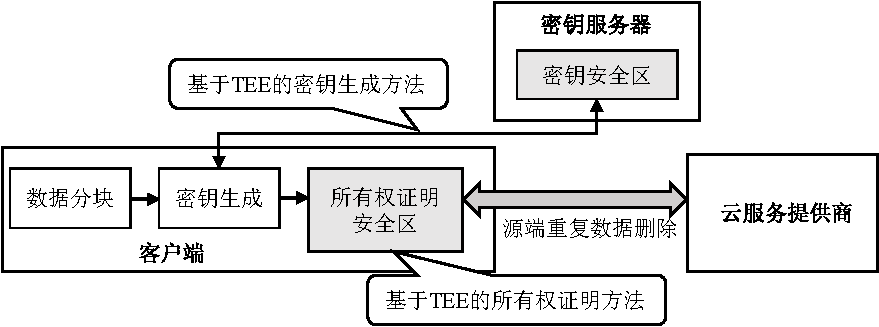
\includegraphics[width=\textwidth]{pic/sgxdedup/sgxdedup-arch.pdf}
    \caption{\sysnameS 系统框架,在密钥服务器和每个客户端中分别部署了密钥安全区和所有权证明安全区}
    \label{fig:sgxdedup-overview}
\end{figure}

\paragraph*{基于密钥安全区的服务器MLE密钥生成。}如图~\ref{fig:sgxdedup-overview-key}所示,\sysnameS 在密钥服务器中部署一个密钥安全区\textit{(Key Enclave)},以管理和保护服务器辅助消息锁加密所需的全局秘密$S$,使其免受恶意(例如,被攻击者攻击并取得控制权限)的密钥服务器的威胁。在执行服务器辅助消息锁加密密钥生成时,密钥安全区和客户端都首先基于共享的会话密钥(Blinded key)建立一个安全信道(有关如何生成会话密钥的详细设计,请参阅\S\ref{subsec:sgxdedup-key-management});然后客户端通过安全信道提交明文数据块的指纹;密钥安全区计算全局秘密和数据块指纹连接的结果的安全哈希作为该指纹对应的消息锁加密密钥;最后,密钥安全区通过安全信道向客户端返回该消息锁加密密钥。

\begin{figure}[!htb]
    \centering
    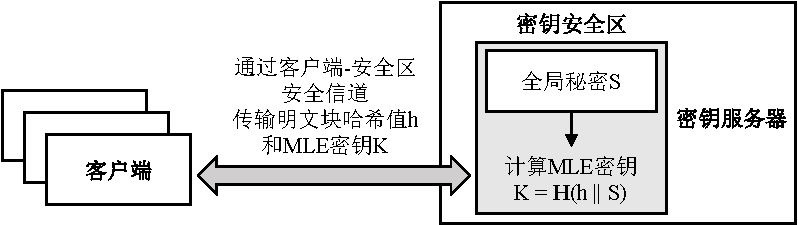
\includegraphics[width=0.9\textwidth]{pic/sgxdedup/key-enclave.pdf}
    \caption{基于密钥安全区的服务器辅助MLE密钥生成}
    \label{fig:sgxdedup-overview-key}
\end{figure}

密钥安全区同时实现了性能和安全性目标,它避免了在消息锁加密密钥生成期间使用昂贵的OPRF协议\cite{bellare2013DupLESS}。此外,它通过基于共享的会话密钥的安全信道保护数据块指纹和消息锁加密密钥,这样密钥服务器就无法从消息锁加密密钥生成过程中学习任何信息。此外,它可以有效保护安全区内存中的全局秘密$S$,即使密钥服务器受到攻击也能避免全局秘密的泄露,保障服务器辅助消息锁加密的安全性。但传统服务器辅助消息锁加密的安全性会由于全局秘密泄露而降低(\S\ref{subsec:background-encrypted-deduplication-key})。



\paragraph*{基于所有权证明安全区的数据块所有权证明。}如图~\ref{fig:sgxdedup-overview-pow}所示,\sysnameS 在每个客户端中部署一个所有权证明安全区,以证明源端重复数据删除中密文数据块的真实性。所有权证明安全区首先与云服务端协商生成一个共享的所有权证明密钥(\textit{PoW}密钥,本文目前使用Diffie-Hellman密钥交换(DHKE)实现密钥协商,参见\S\ref{sec:sgxdedup-implementation})。在生成消息锁加密密钥后,客户端将每个明文数据块加密为密文数据块。所有权证明安全区将密文数据块作为输入,计算相应的指纹,并使用与云服务端共享的PoW密钥创建该指纹的签名。随后,客户端将指纹和签名一起上传到云服务端。云服务端根据客户端对应的PoW密钥及指纹附加的签名验证指纹的真实性。只有当指纹被认证为真实有效时,云服务端才会继续检查指纹是否对应于任何已经存储的密文数据块副本。这里,本文验证客户端对密文数据块的所有权而不是明文的所有权(例如,\cite{halevi11}),以保护原始信息不被云服务端访问。由于消息锁加密产生的密文数据块与明文数据块一一对应,并且密文数据块的所有权与对应的明文数据块的所有权一致。因此,确保密文数据块的所有权足以保证安全。

\begin{figure}[!htb]
    \centering
    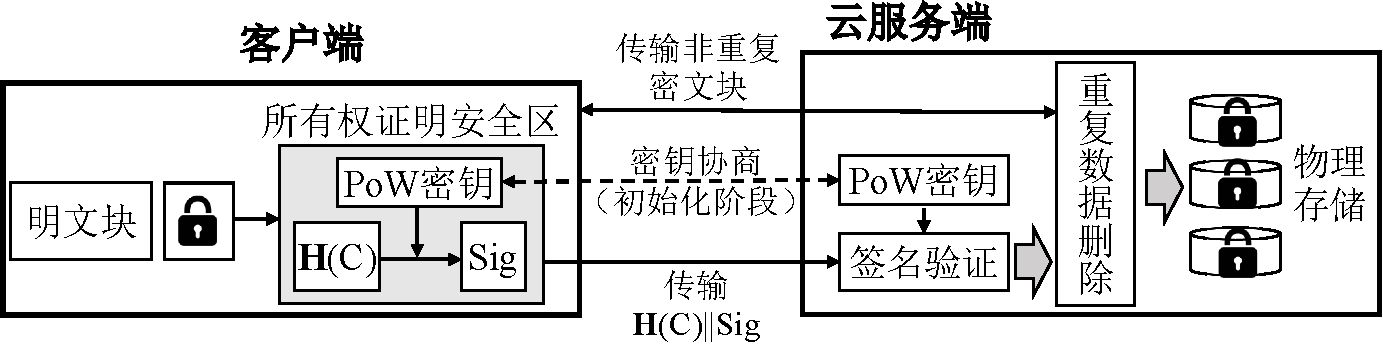
\includegraphics[width=\textwidth]{pic/sgxdedup/pow.pdf}
    \caption{\sysnameS 系统架构: 所有权证明安全区}
    \label{fig:sgxdedup-overview-pow}
\end{figure}


与密钥安全区相似,所有权证明安全区同样可实现效率与安全性的双重设计目标。它避免了基于密码学算法的所有权证明中Merkle树等结构的计算开销。同时,由于数据块是否已被云服务端存储的信息仅在数据块所有权验证通过后才会返回客户端,密钥安全区可有效保护重复数据删除系统免受恶意客户端的伪造数据所有权的攻击威胁。

\textbf{与现有研究\cite{kim2019ShieldStore,fuhry2020segshare,djoko2019NEXUS}在安全区内执行密钥生成和加密不同,本文选择在安全区之外执行数据块加密。}主要原因是原始明文数据块和加密过程都位于客户端内。被攻击的客户端本身可以直接访问其明文数据块,将加密过程移动到安全区内并不能提高安全性,同时还会导致安全区的计算开销增大、可信计算基大小增加。

\begin{table}[!htb]
    \small
    \centering
    \begin{tabular}{ccc}
        \toprule
        {\bf 所属安全区} & {\bf ECall名称}            & {\bf 描述}                                                           \\ 
        \midrule
        \multirow{5}{*}{\bf 密钥安全区}
                         & \textit{Secret generation} & 产生全局秘密 
        (\S\ref{subsec:sgxdedup-enclave-management})                                                                         \\
                         & \textit{Rekeying}          & 更新会话密钥 
        (\S\ref{subsec:sgxdedup-key-management})                                                                             \\
                         & \textit{Nonce checking}    & 检查nonce合规性 
        (\S\ref{subsec:sgxdedup-encryption})                                                                                 \\
                         & \textit{Key generation}    & 产生消息锁加密(MLE)密钥 (\S\ref{subsec:sgxdedup-encryption})         \\
                         & \textit{Mask generation}   & 生成加密掩码 (\S\ref{subsec:sgxdedup-encryption})                    \\
        \hline
        \multirow{3}{*}{\bf 所有权证明安全区}
                         & \textit{Key unsealing}     & 从磁盘解封所有权PoW密钥 (\S\ref{subsec:sgxdedup-enclave-management}) \\
                         & \textit{Key sealing}       & 密封所有权PoW密钥至磁盘 (\S\ref{subsec:sgxdedup-enclave-management}) \\
                         & \textit{Proof generation}  & 签名密文数据块对应的指纹 
        (\S\ref{sec:sgxdedup-implementation})                                                                                \\
        \bottomrule
    \end{tabular}
    \caption{\sysnameS 中的安全区内部调用(Ecalls)}
    \label{tab:sgxdedup-ecall}
\end{table}

\paragraph*{部署安全区存在的问题。}有效地实现基于TEE的加密后重复数据删除并非易事,因为本文需要减轻安全区的潜在性能开销,否则会抵消引入安全区带来的整体性能优势。本文提出了以下三个关键科学问题,并基于一套用于密钥安全区和所有权证明安全区(Table~\ref{tab:sgxdedup-ecall})的安全区内部调用来解决这些问题。

\begin{itemize}[leftmargin=0em]
    \item \textbf{如何安全有效地引导安全区?} (\S\ref{subsec:sgxdedup-enclave-management})由于密钥安全区需要维护全局秘密,在安全区启动时将全局秘密安全地载入密钥安全区中至关重要。此外,所有权证明安全区与客户端深度绑定,它应该在客户端在线访问云服务端时快速且安全的启动,并在客户端退出时以安全有效地方式终止。
    \item \textbf{密钥安全区和每个客户端应该如何建立安全信道?} (\S\ref{subsec:sgxdedup-key-management})
          每个客户端都基于共享的会话密钥与密钥安全区进行安全通信,以便生成必要的消息锁加密密钥来保护外包数据块。由于客户端可能随时加入或退出云存储服务订阅组,会话密钥不仅需要被高效协商产生,而且需要可以动态更新以进行动态客户端认证。
    \item \textbf{密钥安全区应该如何减少管理客户端安全信道的计算开销?} (\S\ref{subsec:sgxdedup-encryption})
          在每个安全信道中(密钥安全区和每个客户端之间),密钥安全区需要解密收到的数据块指纹并加密所生成的消息锁加密密钥。它的计算复杂度随着指纹数量和连接客户端的数量增加而增加。
\end{itemize}

\subsection{安全区管理}
\label{subsec:sgxdedup-enclave-management}

\sysnameS 在首次初始化时通过云建立对所有安全区的信任。在部署 \sysnameS 之前,本文首先将安全区代码编译成共享对象 \cite{sgx},为每个共享对象附加签名(用于完整性验证),并将共享对象分发到密钥服务器和每个客户端。云还托管共享对象以供后续验证。密钥服务器创建密钥安全区,而每个客户端通过加载相应的共享对象来创建自己的所有权证明安全区。云通过远程证明 (\S\ref{subsec:sgxdedup-sgx}) 对每个安全区进行身份验证,以确保加载正确的代码。在这里,本文解决了两个特定的管理问题:(i)如何将全局秘密(\S\ref{subsec:sgxdedup-arch})安全地引导到密钥安全区; (ii) 每个客户端在重启后如何有效地引导其所有权证明安全区。

\paragraph*{Key安全区management.} \sysnameS 不是完全引导全局密钥,而是根据云和密钥服务器分别拥有的两个 \textit{ sub-secrets} 在密钥安全区中生成全局密钥,以便阻止他们中的任何一个了解整个全球秘密。
为了生成全局密钥,本文将云的子密钥硬编码到密钥安全区代码中,并在 \sysnameS 初始化期间将代码(作为共享对象)传递给密钥服务器。本文还为密钥安全区实现了一个\textit{ secret generation ECall},以便让密钥服务器提供自己的子密钥。只有在云的子密钥被包含在密钥安全区中后,密钥服务器才能发出 ECall。它将密钥服务器的子密钥作为其单一输入,并对密钥服务器的子密钥和云的子密钥的串联进行哈希运算,形成全局密钥。请注意,密钥服务器无法访问安全区代码,因此无法了解在安全区内硬编码的云子秘密(假设逆向工程是不可能的)。因此,即使密钥服务器遭到破坏,全局秘密仍然是安全的,因此服务器辅助 消息锁加密(MLE) 的安全性得以保留。如果密钥服务器和云同时受到威胁,\sysnameS 的安全性会降低到原始 消息锁加密(MLE) (\S\ref{subsec:sgxdedup-encrypted-dedup}) 的安全性。

\paragraph*{所有权证明安全区管理。} 当客户端启动其 所有权证明安全区时,它​​需要证明 所有权证明安全区的真实性。但是,远程证明通常会产生非常大的延迟(例如,大约 9\,s;请参阅 \S\ref{subsec:sgxdedup-synthetic})以连接到Intel服务。与 key安全区不同,其远程证明只在初始化期间完成一次,客户端每次加入和离开 \sysnameS 时都需要分别引导和终止 PoW enclave。如果每次客户端加入时都使用远程证明,其大量开销将损害可用性。

\sysnameS 在 所有权证明安全区的第一次引导后利用密封来避免远程证明。回想一下,PoW 安全区与云共享一个PoW Key,这样云就可以验证指纹的真实性 (\S\ref{subsec:sgxdedup-arch})。本文的想法是根据 所有权证明安全区的测量哈希来密封PoW Key。因此,当客户端再次引导其所有权证明安全区时,它会将PoW Key解封到引导的所有权证明安全区中。只要成功恢复PoW Key,就可以验证自举 所有权证明安全区的真实性。

具体来说,客户端首先检查其物理机中是否有任何密封的PoW Key在本地可用。如果密封的PoW Key不可用(第一个引导程序),客户端通过远程证明来证明所有权证明安全区并与云交换PoW Key;否则,如果一个密封的PoW Key可用(在第一次引导之后),客户端通过加载共享对象创建一个新的 PoW enclave,并调用新 所有权证明安全区的 \textit{ key unsealing ECall} 来解封PoW Key。解封 ECall 的密钥以被密封的PoW Key的地址作为输入。它根据新 所有权证明安全区的测量散列推导出密封密钥,解密密封的PoW Key,并将其保存在新的 所有权证明安全区中。

当客户端离开 \sysnameS 时,它​​的 所有权证明安全区需要被终止。客户端发出 \textit{ key seal ECall} 来密封PoW Key。密钥密封 ECall 根据 所有权证明安全区的测量哈希对PoW Key进行加密,并将结果存储在客户端提供的地址中。
\subsection{自更新会话密钥管理}
\label{subsec:sgxdedup-key-management}

每个客户端都通过一个共享的会话密钥与密钥安全区安全通信,以防止密钥服务器 (\S\ref{subsec:sgxdedup-arch})窃听。为了产生会话密钥,一种直接的方法是直接在密钥安全区和每个客户端之间实现密钥协商协议。但是,密钥安全区需要即时验证客户端访问权限(例如,客户端可以更新或撤销其云存储服务订阅)。这种动态认证给密钥安全区带来了性能负担。

\begin{figure}[!htb]
    \centering
    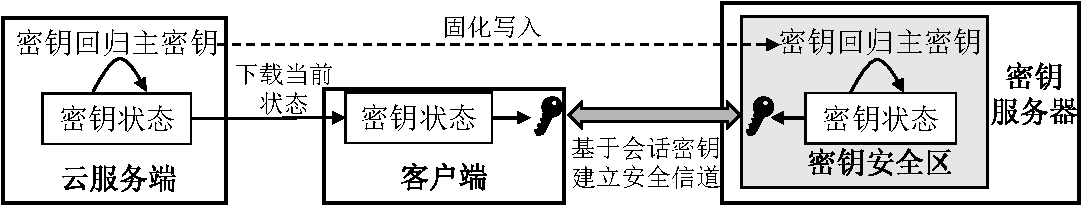
\includegraphics[width=\textwidth]{pic/sgxdedup/keyRegression.pdf}
    \caption{自更新的会话密钥管理:云服务端和密钥安全区可以根据其会话密钥状态导出新的会话密钥,而客户端只能从云服务端下载当前密钥状态,并产生最新的会话密钥}
    \label{fig:sgxdedup-keymanage}
\end{figure}

如图~\ref{fig:sgxdedup-keymanage}所示,\sysnameS 在云服务端的帮助下管理会话密钥。在系统初始化期间,云服务端将一个盲秘密种子$\kappa$硬编码到密钥安全区代码中。每个客户端从云服务端下载一个密钥状态\textit{(key state)}(源自于$\kappa$;见下文),并基于该密钥状态生成对应的会话密钥,用于与密钥安全区的安全通信。本文如此设计的考虑有以下三点:
\begin{itemize}
    \item 首先,当客户端对云服务端发出任何上传/下载请求时,云服务端可以检查客户端是否被授权。
    \item 其次,本文可以从$\kappa$派生(而不是直接使用$\kappa$)一系列自更新的会话密钥,以防止被撤销/被攻击的客户端持续访问密钥安全区。
    \item 自更新密钥管理定期更新会话密钥,要求客户端定期在云服务端进行验证,可以防止在线暴力攻击(\S\ref{subsec:background-encrypted-deduplication-key}),而不会主动降低密钥生成速率\cite{bellare2013DupLESS}。
\end{itemize}

\sysnameS 基于密钥回归(\textit{key regression})\cite{fu06}导出自更新的会话密钥,同时确保每个客户端和密钥安全区中的会话密钥是一致的。具体来说,密钥回归使用一系列密钥状态$S[1]、S[2]、\ldots、S[m]$,每个密钥状态都可用于派生密钥(例如,通过哈希函数)。它允许密钥安全区和云服务端执行密钥状态更新(\textit{rekeying})以使用盲秘密种子从旧密钥状态派生新密钥状态(例如,从$S[1]$导出$S[2]$),使得客户端无法在不知道盲秘密种子的情况下获得有关新密钥状态的任何信息。同时,它允许每个客户端从新密钥状态派生任何旧密钥状态(例如,从$S[2]$派生$S[1]$)。

为了在\sysnameS 中实现密钥回归,本文使用$\kappa$作为在云服务端和密钥安全区之间共享的盲秘密种子,用于派生新的密钥状态和会话密钥。在每次上传开始前,客户端首先从云服务端下载最新的密钥状态$S[i]$,并向密钥服务器查询密钥安全区接受的会话密钥的版本号$j$。鉴于密钥安全区可能无法及时更新会话密钥(例如,在计划的更新密钥时间内正在提供密钥生成服务),$j$通常小于$i$(即$S[j]$在$S[i]$之前)。然后客户端从$S[i]$派生出$S[j]$并导出对应的会话密钥$K[j]$,最终基于相同的$K[j]$与密钥安全区通信。请注意,云服务端可以导出$K[j]$,但它无法窃听每个客户端和密钥安全区之间的通信,因为通过客户端和密钥服务器之间的通信受到SSL/TLS协议的额外保护(参见本文在\S\ref{subsec:sgxdedup-threat} 中提出的安全假设)。

\sysnameS 在云服务端和密钥服务器中实现了同步计时器,在周期性的时间间隔内自动触发会话密钥更新。这里,密钥服务器发出\textit{Rekeying ECall}以在达到预定的密钥更新时间且密钥服务器结束对已连接客户端的服务时通过安全区内部调用触发安全区内会话密钥更新。

本文实现了基于哈希的密钥回归方案\cite{fu06}以获得较高的密钥更新性能。具体来说,本文定义了参数$n$(默认设置为$2^{20}$\cite{fu06})来指示可进行的最大密钥更新次数。 云服务端和密钥安全区计算第$i$个密钥状态为$S[i] = {\bf H}^{n-i+1}(\kappa)$,每个客户端派生相应的会话密钥为$K[i] = {\bf H}(S[i] || 0^8)$,其中${\bf H}^{n-i+1}()$迭代调用安全哈希函数${\bf H}()$共计$n-i+1$次,$||$是连接运算符。若客户端需要导出旧密钥$K[j]$,则客户端下载$S[i]$并计算$S[i-1] = {\bf H}(S[i])$直到得到目标密钥状态$S[j]$,进而导出会话密钥$K[j] = {\bf H}(S[j] || 0^8)$。

\subsection{基于 SGX 的推测性加密}
\label{subsec:sgxdedup-encryption}

给定共享盲密钥 (\S\ref{subsec:sgxdedup-key-management}),密钥安全区管理与每个客户端的安全通道,以在 消息锁加密(MLE) 密钥生成期间保护传输的指纹/密钥 (\S\ref{subsec:sgxdedup-arch} )。然而,管理安全通道,特别是对于许多客户端,会在密钥安全区中产生高昂的加密/解密成本。 \sysnameS 在 SGX 的上下文中使用 \textit{ 推测性加密} \cite{eduardo19} 增强了安全通信通道管理,从而减轻了密钥安全区的加密/解密开销。

\paragraph*{推测性加密} 推测性加密 \cite{eduardo19} 采用\textit{计数器模式(CTR)} \cite{counter} 加解密,在离线过程中预先计算部分加解密结果,以减少在线独立加密文件系统中的计算开销。为了加密明文 $M$,本文首先将 $M$ 划分为一系列明文数据块 $b_1、b_2、\ldots、b_m$(例如,每个块的大小固定为 16 字节)。对于每个客户端,本文选择一个唯一的 \textit{ nonce} $\theta$,它只能被使用相同密钥的加密使用一次。然后本文计算第 $i$ 个明文数据块的 \textit{掩码}为 $e_i = {\bf E}(K, \theta || i)$,其中 ${\bf E}()$ 是对称加密函数,$K$ 是密钥,$i$ 是 \textit{ counter}(用于计数器模式加密),`$||$' 是连接运算符。最后,本文计算每个密文数据块$c_i = e_i \oplus b_i $,其中$\oplus$是按位异或运算符,并形成整个密文$C = c_1 || c_2 || \ldots || c_m$。为了解密密文,本文像上面一样为每个块生成掩码 $e_i$,恢复相应的明文数据块 $b_i = e_i \oplus c_i$ 并因此恢复原始明文 $M$。由于掩码生成步骤独立于每个目标明文/密文,本文可以离线预先计算掩码,然后应用轻量级 XOR 操作进行在线加密/解密。

\begin{figure}[t]
\centering
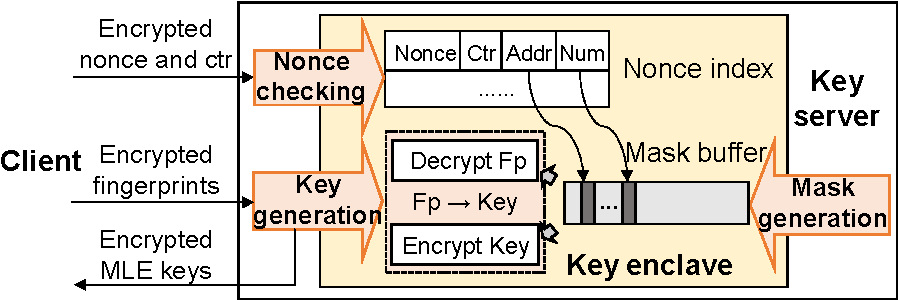
\includegraphics[width=\textwidth]{pic/sgxdedup/encryption.pdf}
\caption{Overview of SGX-based speculative encryption.}
\label{fig:sgxdedup-SpecEnc}
\end{figure}

\paragraph*{Integration.} 要在 \sysnameS 中实现推测性加密,本文需要解决 nonce、管理问题。、唯一的 nonce 充当不可预测的“一次性填充”,使得、每个 counter-mode 加密输出看起来随机 \cite{counter}。如果多个客户端使用反模式加密,本文需要在每个客户端的加密/解密操作中关联一个唯一的 nonce。但是,由于不同的客户端是隔离的,因此很难确保关联的 nonce客户是独一无二的。

为了确保 nonce 的唯一性,\sysnameS 在 key安全区中管理一个集中的 key-value 存储,称为 \textit{ nonce index}。 nonce 索引的每个条目将存储的 nonce(12 字节)映射到三个字段:其计数器(4 字节)、相应掩码的起始地址(8 字节)和可用掩码的数量(4 字节)。此外,\sysnameS 实现了一个 \textit{ nonce checks ECall} (Figure~\ref{fig:sgxdedup-SpecEnc}),它可以被密钥管理器调用,以将每个客户端提交的 nonce 与之前存储在 nonce 索引中的 nonce 进行比较,并如果发现重复的 nonce,通知客户重新选择一个新的。请注意,可以有效管理 in-enclave 随机数索引,因为它可以服务多达 112,000 个客户端(假设每个客户端一个随机数),只有 3MB EPC 空间(默认配置为 \sysnameS)。

\sysnameS 应用推测性加密在客户端和密钥安全区之间建立安全通道,以保护 消息锁加密(MLE) 密钥生成。为了初始化安全通道,客户端将其自行选择的随机数 $\theta$ 和对应的计数器 $i$ 与密钥安全区同步,如果 $\theta$ 未用于任何加密,则 $i$ 初始化为零/由客户端解密。具体来说,它使用最新的盲密钥 (\S\ref{subsec:sgxdedup-key-management}) 加密 $\theta$ 和 $i$,根据生成的密文计算消息验证码 (MAC),并将密文和 MAC 提交给密钥管理器。在这里,本文采用 \textit{ encrypt-then-MAC} \cite{bellare2000Authenticated} 通过检查 MAC 中的客户端和密钥安全区之间传输的任何信息来检测任何过时的盲密钥。

密钥管理器发出随机数检查 ECall,它将客户端的上传作为输入,解密 $\theta$ 和 $i$,并使用随机数索引检查解密后的 $\theta$ 和 $i$:
%
\begin{itemize}[leftmargin=*]
\item Case I:如果$\theta$ 是重复的并且$i$ = 0,这表示重复使用现有的nonce,并且ECall 返回一个信号通知客户端重新选择一个新的nonce。
\item 案例二:如果 $\theta$ 是重复的并且 $i \neq$ 为 0,这意味着 nonce 已被存储。 ECall 更新存储的计数器并标记相应的预计算掩码(用于后续处理,如下所述)。
\item 案例 III:如果 $\theta$ 是唯一的,这意味着 nonce 是新的,并且 ECall 将 $\theta$ 添加到 nonce 索引中。
\end{itemize}

对于 Cases~II 和 III,ECall 接受通信并要求客户端传输指纹以生成 消息锁加密(MLE) 密钥 (\S\ref{subsec:sgxdedup-arch})。客户端根据$\theta$和$i$对指纹进行加密,并上​​传结果;在加密每个指纹块后,客户端将 $i$ 加一以防止重放攻击。如图~\ref{fig:sgxdedup-SpecEnc}所示,密钥管理器发出\textit{ key generation ECall}来处理加密的指纹。 ECall 检查是否为当前客户端标记了某些掩码。如果找到(即情况 II),它使用标记的掩码来解密指纹并加密生成的 消息锁加密(MLE) 密钥。否则(即案例 III),它会在线计算掩码以进行解密和加密。

\paragraph*{掩码预计算。} 为了加速加密/解密,当应用新的盲密钥(即所有现有掩码无效)或客户端在最后一个掩码后再次连接时,密钥安全区会执行掩码预计算代(即,它的一些掩码已被消耗)。关键安全区调用 \textit{ 掩码生成 ECall}(图~\ref{fig:sgxdedup-SpecEnc}),它预先计算最近使用的随机数的数量(例如,在本文的例子中为三个)的掩码并写入将结果放入 \textit{ 掩码缓冲区}。默认情况下,本文将掩码缓冲区配置为最大 90\,MB。假设每个掩码占用 16 个字节,平均块大小为 8\,KB。指纹的 消息锁加密(MLE) 密钥生成使用四个掩码:两个用于解密 32 字节指纹,另外两个用于加密生成的 32 字节 消息锁加密(MLE) 密钥。因此,掩码缓冲区中预先计算的掩码可用于处理高达 11.25GB 数据的指纹。

\section{\sysnameS 实现}
\label{sec:sgxdedup-implementation}

本文基于OpenSSL 1.1.1l\citing{openssl}、SGX SDK 2.15\citing{sgxsdk} 、和Intel SGX SSL\citing{sgxssl}使用C++实现了一个\sysnameS 原型系统。本文的原型系统通过SHA-256哈希函数实现明文和密文数据块的指纹计算和识别等操作,并通过AES-256加密算法实现基于数据块的加密机制。原型系统约包含14,200行代码。原型系统源码及操作指南开源于:\href{https://github.com/tinoryj/SGXDedup}{https://github.com/tinoryj/SGXDedup}。

\paragraph*{原型系统启动。}
为了启动密钥安全区,云服务端将对其用于全局秘密生成的子秘密(\S\ref{subsec:sgxdedup-enclave-management})和会话密钥种子(\S\ref{subsec:sgxdedup-key-management})硬编码到密钥安全区动态运行库中。\sysnameS 中云服务端也可以在验证密钥安全区后再通过安全信道向密钥安全区装载子秘密和会话密钥种子(使用SGX\citing{sgx}的秘密提供(Secret provisioning)功能),但会产生额外的启动开销。密钥安全区使用SHA-256哈希算法生成全局秘密并在密钥回归中进行密钥状态更新和会话密钥导出。所有权证明安全区在NIST P-256椭圆曲线\citing{nist}上实现DHKE,以与云服务端共享PoW密钥。

\paragraph*{密钥生成。}每个客户端实现了基于Rabin指纹\citing{rabin81}的内容定义的数据块分块。本文将可变大小分块算法中的最小、平均和最大数据块大小分别固定为4\,KiB,8\,KiB和16\,KiB。为了实现基于TEE的推测性加密(\S\ref{subsec:sgxdedup-encryption}),本文将nonce和计数器长度分别固定为12字节和4字节,并使用HMAC-SHA-256实现消息认证算法。此外,密钥安全区通过SHA-256哈希算法生成每个明文数据块指纹对应的消息锁加密密钥。此外,为了防止恶意客户端使用过期的会话密钥进行密钥生成等操作,客户端与密钥安全区之间通过安全信道传输的所有数据内容(包括:数据块指纹、生成的密钥、初始化所用的nonce和计数器等)均基于会话密钥产生哈希消息认证码,用于检验传输的数据。

\paragraph*{重复数据删除。}\sysnameS 实现了源端重复数据删除与数据块级所有权证明的结合。所有权证明安全区实现了所有权证明安全区内部调用(\textit{Proof generation ECall})来计算密文数据块的指纹,并使用AES-CMAC对生成的指纹生进行签名。云服务端基于LevelDB\citing{leveldb}键值对数据库实现重复数据删除指纹索引(\S\ref{subsec:sgxdedup-problem})。为了降低网络和磁盘I/O开销,本文将非重复密文数据块存储在8\,MiB的容器中,作为传输和存储的基本单位\citing{lillibridge13}。

\paragraph*{系统优化。}为了减少频繁进出安全区导致的CPU上下文切换和安全区内存加密/解密开销,每个客户端批量处理多个明文数据块指纹(默认为4,096个)进行密钥生成请求并在与密钥安全区(\S\ref{subsec:sgxdedup-encryption})之间的安全信道中传输。密钥安全区通过指针访问未受保护的内存读取数据块指纹进行批量消息锁加密密钥生成,而不将指纹内容复制到安全区\citing{harnik2018SGX}。类似地,所有权证明安全区按批次(默认为4,096)处理密文数据块且不复制密文数据块内容到安全区内。本文还使用多线程来提高性能,每个客户端通过多线程并行处理文件分块、明文数据块计算、密钥生成及加密、所有权证明和非重复数据块及元数据上传。同时,密钥安全区和云服务端使用不同线程处理多个客户端的连接。
% evaluation
\section{实验分析}
\label{sec:sgxdedup-evaluation}

本文以多个客户端、密钥服务器和云服务端配置了一个局域网本地验证集群。集群中每台设备均使用四核3.0\,GHz的Intel Core i5-7400 CPU,1\,TB 7200转SATA机械硬和8\,GB DDR4内存。所有设备均运行Ubuntu 18.04 LTS操作系统并通过万兆网络(10\,GbE)连接。本文首先对\sysnameS 中提出的基于TEE的服务器辅助密钥生成和数据所有权证明模块进行性能测试分析(\S\ref{subsec:sgxdedup-synthetic},Exp\#1$\sim$6),随后使用随机(\S\ref{subsec:sgxdedup-synthetic},Exp\#7$\sim$10)和真实世界(\S\ref{subsec:sgxdedup-real-world},Exp\#11$\sim$12)工作负载来评估\sysnameS 的整体性能表现。本文将主要结果总结如下:

\begin{itemize}
    \item \sysnameS 在单客户端(Exp\#1)和多客户端并发(Exp\#2)的条件下均实现了高消息锁加密密钥生成性能。例如,在单客户端情况下,相较于{\em DupLESS}\cite{bellare2013DupLESS}中基于OPRF-RSA的消息锁加密密钥生成实现了131.9倍的性能提升。
    \item \sysnameS 与仅实现较弱的安全性的基于通用哈希的数据所有权证明方案(PoW-UH)\cite{xu2013weak}和实现较高安全性的基于默克尔树的数据所有权证明方案(PoW-MT)\cite{halevi11}相比,分别实现了2.2倍和8.2倍的计算性能提升(Exp\#5)。
    \item \sysnameS 在单客户端(Exp\#7和Exp\#8)和多客户端(Exp\#9)情况下具有较高的整体性能。本文还提供了上传中 \sysnameS 各个步骤的时间开销分析(Exp\#10)。例如,在10\,GbE本地局域网测试平台中,与没有任何安全保护的普通重复数据删除系统(PlainDedup)相比,\sysnameS 的上传速度仅降低了17.5\%;在真实云环境部署(Exp\#8)中,相较于普通重复数据删除系统,\sysnameS 仅产生了13.2\%的性能下降(两者上传性能均受到网络带宽限制)。
    \item 在上传过程的各个步骤时间开销分析中,\sysnameS 将第二次上传(完全重复数据)的客户端初始化时间减少了91.5\%,并将第二次上传的密钥生成时间开销减少了41.9\%(Exp\#10)。
    \item \sysnameS 对于处理实际工作负载(Exp\#11和Exp\#12)非常有效。例如其上传的额外性能开销相对于普通重复数据删除(无安全保护)在22.0\%以内(Exp\#11);与现有方法\cite{li15,harnik2010side} 相比,它还实现了高带宽节省,网络流量开销绝对差异高达91.4\%(Exp\#12)。
\end{itemize}

如表~\ref{tab:sgxdedup-summary}所示,总结了本文提出的基于TEE的高性能加密重复数据删除系统\sysnameS 中各项关键技术以及整体性能相较于现有方案的优劣。

\begin{table}
  \centering
  \small
  \begin{tabular}{cccc}
    \toprule
    \multicolumn{2}{c}{\bf 对比对象} & {\bf 基础方案/系统} & {\bf 优势} \\
    \midrule
    \multirow{8}{*}{\bf 性能提升} & \multirow{4}{*}{\shortstack{密钥生成}} & OPRF-BLS \cite{armknecht2015transparent} & 1,583$\times\;\uparrow$  \\
               &            & OPRF-RSA \cite{bellare2013DupLESS} & 131.9$\times\;\uparrow$ \\
               &            & MinHash encryption \cite{li2020Info} & 9.4$\times\;\uparrow$ \\
               &            & TED \cite{li2020TED} & 3.7$\times\;\uparrow$ \\
    \cline{2-4}
    & \multirow{2}{*}{所有权证明} & PoW-MT \cite{halevi11} & 8.2$\times\;\uparrow$ \\
      &                     & PoW-UH \cite{xu2013weak} & 2.2$\times\;\uparrow$ \\
    \cline{2-4}
    & \multirow{2}{*}{\shortstack{原型系统}} & {\em DupLESS} \cite{bellare2013DupLESS} & 8.1$\times\;\uparrow$ \\
    & & PlainDedup & 17.5\% $\downarrow$ \\
    \hline
    \multicolumn{2}{c}{\multirow{2}{*}{\shortstack{\bf 网络资源节省}}} & Two-stage dedup \cite{li15} & 35.3\% $\uparrow$ \\
\multicolumn{2}{c}{} & Randomized-threshold dedup \cite{harnik2010side} & 91.4\% $\uparrow$ \\
    \bottomrule
  \end{tabular}
    \caption{Summary of main results.}
  \label{tab:sgxdedup-summary}
\end{table}


\subsection{综合工作负载评估}
\label{subsec:synthetic}


我们使用一组文件生成一个合成数据集,每个文件都包含全局非重复块。 默认情况下,我们将文件大小设置为 2\,GB(Exp\#2 除外,我们在其中对 消息锁加密(MLE) 密钥生成性能进行了压力测试)。 客户端通过云上传或下载文件。 为了避免磁盘 I/O 对性能的影响,我们将文件数据存储在内存中而不是磁盘上(Exp\#5 除外,我们在实云部署中处理磁盘上的文件)。 我们绘制了 10 次运行的平均结果。 我们还将 \textit{ Student's t-Distribution} 的 95\% 置信区间包含在条形图中(为简洁起见,我们将它们从折线图中排除)。


\begin{figure}[!htb]
\centering
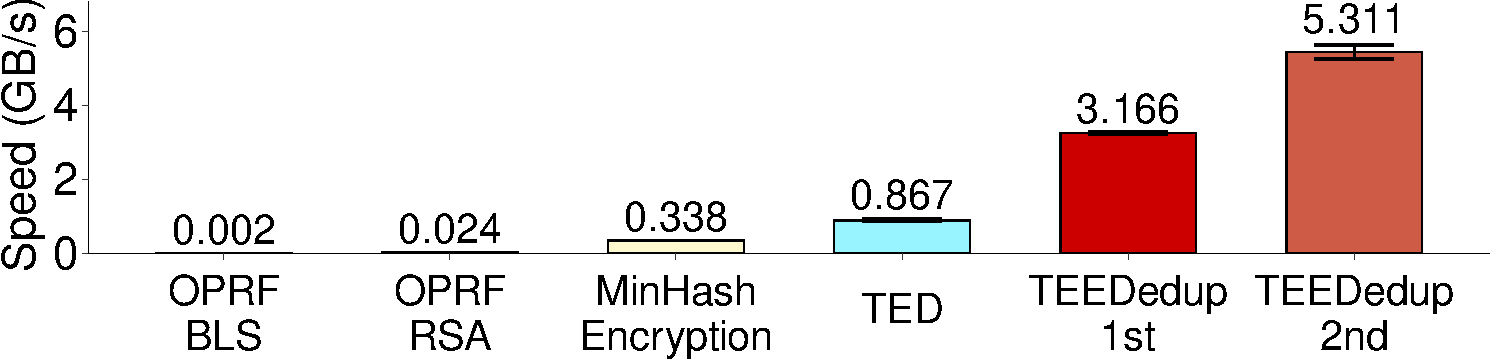
\includegraphics[width=\textwidth]{pic/sgxdedup/expa2_keyGenPerformance.pdf}
\vspace{-12pt}
\caption{(Exp\#1) Single-client 消息锁加密(MLE) key generation.}
\label{fig:keygen-comparison}
\end{figure}

\begin{figure}[!htb]
  \begin{minipage}[t]{0.47\textwidth}
  \centering
  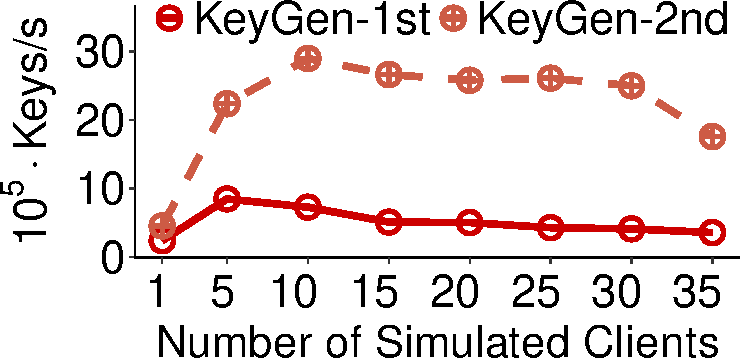
\includegraphics[width=\linewidth]{pic/sgxdedup/expa3_keyScale_performance_number_multiThread.pdf}
  \vspace{-12pt}
  \caption{(Exp\#2) Multi-client 消息锁加密(MLE) key generation.}
  \label{fig:exp-keygen-scalability}
  \end{minipage}%
  \hspace{0.2in}
  \begin{minipage}[t]{0.47\textwidth}
  \centering
  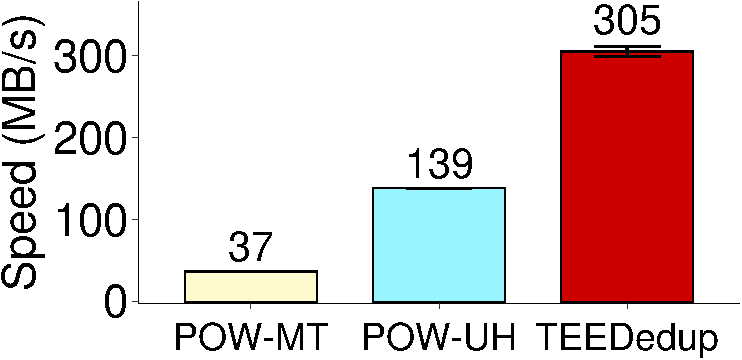
\includegraphics[width=\linewidth]{pic/sgxdedup/expa4_powPerformance.pdf}
  \vspace{-12pt}
  \caption{\small(Exp\#3) Computational PoW.}
  \label{fig:pow-comparison}
  \end{minipage}%
  \vspace{-6pt}
\end{figure}


\paragraph{Exp\#1(单客户端 消息锁加密(MLE) 密钥生成)。} 我们在两轮中评估 消息锁加密(MLE) 密钥生成。首先,客户端通过 Rabin 指纹 (\S\ref{sec:implementation}) 创建 2\,GB 文件的明文块并发出 消息锁加密(MLE) 密钥生成请求。然后它为不同的 2\,GB 文件的块重复 消息锁加密(MLE) 密钥生成过程。不同之处在于第二轮使用预先计算的掩码生成 消息锁加密(MLE) 密钥 (\S\ref{subsec:encryption})。

我们将 \sysnameS 的单客户端 消息锁加密(MLE) 密钥生成速度与最新技术进行了比较。我们考虑两种基于 OPRF 的密钥生成方法,即 \textit{ OPRF-BLS} \cite{armknecht15} 和 \textit{ OPRF-RSA} \cite{bellare13b},它们实现了 OPRF 原语(\S\ref{subsec:encrypted-dedup})分别基于盲 BLS 和盲 RSA 签名。我们还考虑了两种宽松的密钥生成方法,即 \textit{ MinHash encryption} \cite{qin17} 和 \textit{ TED} \cite{li20b},它们以存储效率和安全性换取性能。具体来说,MinHash 加密使用 OPRF-RSA 在每个段的基础上生成 消息锁加密(MLE) 密钥,其中平均段大小配置为 1\,MB。 TED 根据块的短散列的基于草图的频率计数为每个块生成 消息锁加密(MLE) 密钥(参见 \cite{li20b} 中的 \S3.3)。

图~\ref{fig:keygen-comparison} 显示了结果。 \sysnameS 通过避免 OPRF-BLS、OPRF-RSA 和 MinHash 加密中昂贵的密码原语以及 TED 中的频率计数计算,优于所有基线方法。它的第一轮分别比 OPRF-BLS 和 OPRF-RSA 实现了 1,583$\times$ 和 131.9$\times$ 的加速。与 MinHash 加密和 TED 相比,加速分别为 9.4$\times$ 和 3.7$\times$,尽管后两者牺牲了存储效率和安全性。第二轮投机加密将第一轮的 消息锁加密(MLE) 密钥生成速度提高了 67.8\%。



\paragraph{Exp\#2(多客户端 消息锁加密(MLE) 密钥生成)。} 我们评估多客户端 消息锁加密(MLE) 密钥生成。对于压力测试,我们配置了一台运行多个线程的机器,每个线程都模拟一个客户端,同时向密钥管理器(在不同的机器上运行)发出 消息锁加密(MLE) 密钥生成请求。回想一下,密钥安全区中预先计算的掩码可用于有效处理最多 11.25GB 的数据 (\S\ref{subsec:encryption})。为了在第二轮中为每个模拟客户端启用推测加密,我们将每个线程配置为生成 40,960 个指纹(即 320 个,8 个 KB 块的 MB 原始数据),并将密钥安全区配置为同等地预先计算掩码每个模拟客户端在第一轮密钥生成之后。我们在处理来自所有模拟客户端的所有 消息锁加密(MLE) 密钥生成请求时测量 \textit{ aggregate} 消息锁加密(MLE) 密钥生成速度。

图~\ref{fig:exp-keygen-scalability} 展示了结果。两轮的总密钥生成速度最初随着模拟客户端的数量而增加。在高峰期,第一轮和第二轮分别为 5 个和 10 个模拟客户端实现了 $8.5\times 10^5$\,keys/s 和 $29\times 10^5$\,keys/s。在十个客户端之后,由于加重的上下文切换开销,聚合速度下降。平均而言,第二轮的投机加密比第一轮实现了 4.4$\times$ 的聚合密钥生成加速。


\paragraph{Exp\#3 (Computational PoW).} 我们评估 PoW 的性能。我们考虑一个对 2GB 文件执行 PoW 的客户端。客户端从文件中创建明文块,加密每个明文块,并向云端发出 PoW 请求。我们根据客户端(PoW enclave 对密文块执行指纹识别并签署结果指纹)和云(验证数据的真实性)中所有块的总计算时间来测量 \textit{ 计算 PoW 速度}指纹);请注意,我们在速度计算中排除了客户端和云端之间的网络传输时间(我们在附录中的 Exp\#11 中考虑了网络传输时间)。

我们将 \sysnameS 与两种最先进的 PoW 方法进行比较:(i) \textit{ PoW-MT} \cite{halevi11}(又名 \cite{halevi11} 中的基本版本), PoW 方法使用纠删码对块进行编码,并在 PoW 的编码内容上构建 Merkle 树; (ii) \textit{ PoW-UH} \cite{xu13},它建立在通用散列之上,但以安全性换取性能。为了公平比较,我们自己在 C++ 中实现了 PoW-MT 和 PoW-UH。请注意,有改进的 PoW 方法 \cite{halevi11},但它们会因低内存使用而产生更高的性能开销。


图~\ref{fig:pow-comparison} 显示了结果。 \sysnameS 显着优于 PoW-MT,因为它避免了客户端中的擦除编码和 Merkle 树构造,以及云中基于 Merkle 树的验证。 它比 PoW-MT 实现了 8.2$\times$ 的加速。 它还比 PoW-UH 实现了 2.2$\times$ 的加速。


\begin{figure}[t]
  \centering
  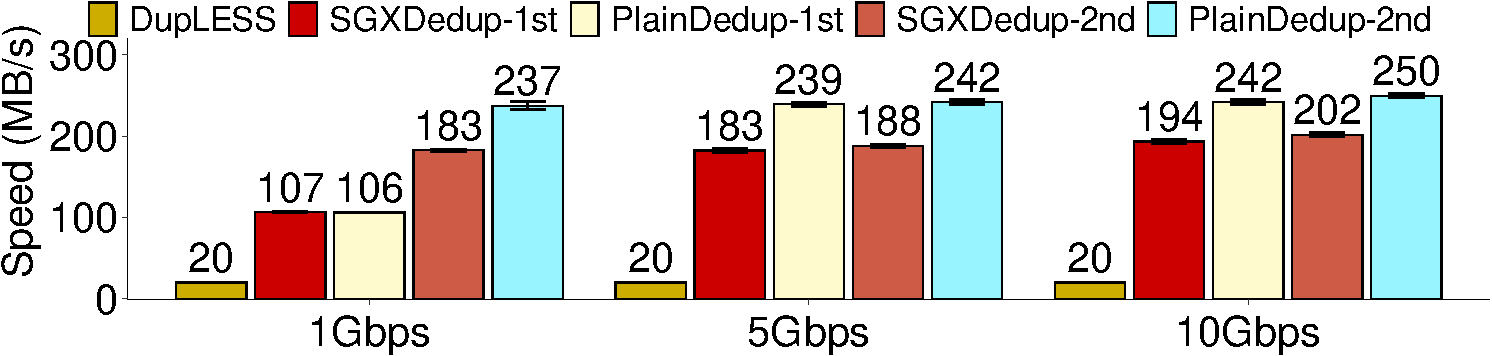
\includegraphics[width=0.6\textwidth]{pic/sgxdedup/upload_network_speed_bar.pdf} \ \ 
  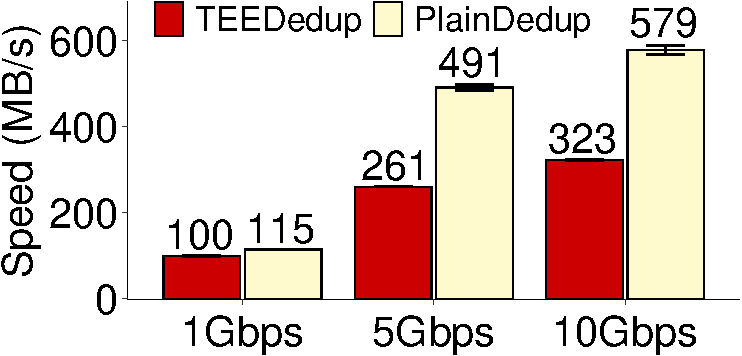
\includegraphics[width=0.3\textwidth]{pic/sgxdedup/download_network_speed_bar.pdf}
  \vspace{-3pt}\\
    \hspace{1.1in} {\small (a) Upload} \hspace{1.9in}
  {\small (b) Download}
  \vspace{-6pt}\\
  \caption{(Exp\#4) Single-client uploads and downloads. We exclude the second upload speed of DupLESS (which has the same performance in two uploads) and the download speed of DupLESS (which is identical to that of  \sysnameS).}
  \label{fig:singleClientThroughput}
\end{figure}

\begin{figure}[t]
  \centering
  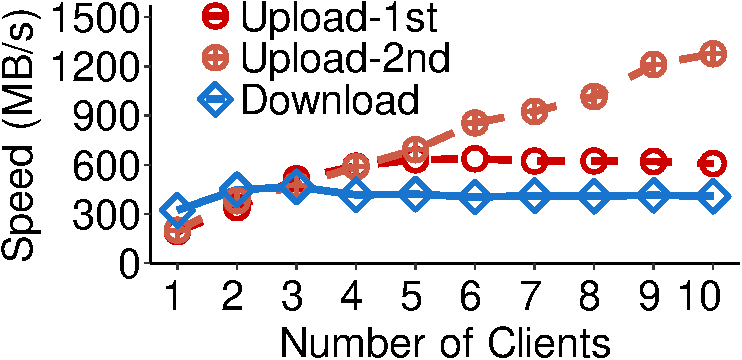
\includegraphics[width=0.6\textwidth]{pic/sgxdedup/expb1_multiple_client.pdf}  
  \caption{(Exp\#6) Multi-client uploads and downloads.}
  \label{fig:multiClientThroughput}
\end{figure}

\paragraph{Exp\#4 (Single-client uploads and downloads).} 我们考虑单个客户端,并将 \sysnameS 的上传和下载性能与两个基线系统进行比较:(i) \textit{ PlainDedup},禁用 \sysnameS 的密钥生成、加密和PoW操作,从而实现基于源的去重,无需任何安全保护; (ii) \textit{ DupLESS} \cite{bellare13b},它通过 OPRF-RSA 生成每块 消息锁加密(MLE) 密钥,执行加密并将所有密文块上传到云以进行重复数据删除。由于 DupLESS 的原始实现不提供去重存储后端(假设使用了 Dropbox),我们根据 \cite{bellare13b} 中描述的设计在 C++ 中实现 DupLESS。请注意,PlainDedup 基于未加密的文件元数据检索文件,并且不同于加密重复数据删除系统中的两轮下载(即 \sysnameS 和 DupLESS);在后者中,客户端首先下载并解密文件元数据,然后下载块以重建文件 (\S\ref{subsec:encrypted-dedup})。

我们分三个步骤评估上传和下载速度: (i) 客户端首先上传 2\,GB 文件; (ii) 客户端重新启动,然后上传另一个与前一个相同的 2\,GB 文件; (iii) 客户端下载文件。请注意,第二次上传执行基于源的重复数据删除(对于 PlainDedup 和 \sysnameS),并利用预先计算的掩码来加速密钥生成(仅适用于 \sysnameS)。

图~\ref{fig:singleClientThroughput}(a) 显示了由 {\tt trickle} \cite{eriksen05} 控制的不同网络带宽的上传速度。第一次上传,当网络带宽为 1\,Gbps 时,\sysnameS (106.6\,MB/s) 和 PlainDedup (106.2\,MB/s) 的上传速度均受网速约束,而性能DupLESS (20.1\,MB/s) 的瓶颈是基于 OPRF-RSA 的密钥生成 (Exp\#1)。当网络带宽增加到 10\,Gbps(默认)时,\sysnameS 和 PlainDedup 的上传速度分别达到 193.6\,MB/s 和 242.0\,MB/s,而 DupLESS 的上传速度稳定在 20.0\, MB/秒。对于第二次上传,由于其密钥生成性能瓶颈,DupLESS 达到了与第一次上传相同的速度。 \sysnameS 和 PlainDedup 的上传速度受网络带宽的影响较小,因为它们不需要传输数据。平均而言,\sysnameS 在第一次和第二次上传中分别比 DupLESS 实现了 8.1$\times$ 和 9.6$\times$ 的加速。即使与不安全的 PlainDedup 相比,\sysnameS 也只会导致相应的上传速度下降约 17.5\% 和 21.4\%。开销来自 \sysnameS 的安全机制,包括密钥生成、加密和 PoW。

图~\ref{fig:singleClientThroughput}(b) 显示了下载速度。随着网络带宽增加到 10\,Gbps,\sysnameS 和 DupLESS 均达到 323.1\,MB/s,比 PlainDedup 下降了 44.2\%。原因是他们连续检索和解密文件元数据,然后下载密文块。

\paragraph{Exp\#5(真实云上传和下载)。} 我们现在扩展 Exp\#4 并评估真实云部署中的上传和下载速度。具体来说,我们将客户端和密钥管理器部署在我们的局域网测试平台(\S\ref{sec:evaluation})中,并通过互联网将客户端连接到\textit{ 阿里云},我们在其中租用了一个虚拟机\textit{ ecs.c6e.xlarge} 运行云。云机配备四核3.2GHz CPU(其主机平台为Intel Xeon Cascade Lake Platinum 8269CY),8GB内存。我们以 \textit{ Alibaba General Purpose NAS} 作为存储后端来挂载云。 NAS 可以实现高达 20000\,IOPS 的 4\,K 次随机读写。

我们使用磁盘上的数据文件进行上传(与 Exp\#4 相对,后者在上传之前将文件加载到客户端的内存中),并允许云端将接收到的数据文件存储在 NAS 中。我们还使用 {\tt scp} 将整个数据文件(即 2\,GB)从客户端上传到云端,以提供互联网环境下的数据传输基准。


Table~\ref{tab:real-cloud} 显示了结果。在第一次上传时,所有系统的性能(\sysnameS 为 11.4\,MB/s,PlainDedup 为 11.6\,MB/s,DupLESS 为 10.8\,MB/s)受限于 Internet 带宽(11.9\,MB/ s)。在第二次上传中,\sysnameS 实现了 104.3\,MB/s,与 DupLESS 相比加速了 9.7$\times$,与 PlainDedup 相比下降了 13.2\%。请注意,性能差异比 Exp\#4 中的要小,因为 \sysnameS 和 PlainDedup 现在受客户端磁盘 I/O 的限制。在下载中,这三个系统的性能再次受到 Internet 带宽的限制,而 \sysnameS 和 DupLESS 由于它们的串行检索和解密(Exp\#4),将 PlainDedup 的下载速度降低了 10.6\%。

\begin{table}[t]
\small
\centering
\renewcommand{\arraystretch}{1.05}
\begin{tabular}{|c|c|c|c|}
\hline
{\bf Approach} & {\bf First Upload} & {\bf Second Upload} & {\bf Download} \\
\hline
\hline
Transfer & \multicolumn{3}{c|}{11.9 $\pm$ 0.03} \\  
\hline
\hline
\sysnameS & 11.4 $\pm$ 0.3 & 104.3 $\pm$ 1.2 & 10.1 $\pm$ 0.1 \\ 
\hline
PlainDedup & 11.6 $\pm$ 0.1 & 120.1 $\pm$ 1.4 & 11.3 $\pm$ 0.3 \\
\hline
DupLESS & \multicolumn{2}{c|}{10.8 $\pm$ 0.2}  & 10.1 $\pm$ 0.1 \\
\hline
\end{tabular}
\vspace{-3pt}
\caption{(Exp\#5) Real-cloud upload and download (unit: MB/s).} 
\label{tab:real-cloud}
\vspace{-6pt}
\end{table}

\paragraph{Exp\#6(多客户端上传和下载)。}我们现在考虑同时发布上传/下载的多个客户端。我们专注于 \sysnameS,并将密钥 enclave 配置为在第一次上传后为每个客户端同等地预先计算掩码。我们将网络带宽固定为 10\,Gbps,并评估所有客户端完成上传/下载的 \textit{ aggregate} 上传和下载速度。

图~\ref{fig:multiClientThroughput} 显示了多达 10 个客户端的结果。第二轮的总上传速度随着客户端数量的增加而增加,达到1277.1\,MB/s。另一方面,由于客户端之间的写竞争,第一轮的总上传速度增加了七个客户端的 637.0MB/s,随后下降到 10 个客户端的 620.3MB/s。同样,由于多个客户端的读取竞争,总下载速度最终下降到 408.8\,MB/s。

\paragraph{Exp\#7(时间分解)。} 我们提供 \sysnameS 的时间分解来研究不同步骤的性能。假设key enclave已经启动,我们关注单个客户端的初始化和上传过程。初始化过程引导客户端的 PoW 安全区。上传过程包括以下步骤: (i) \textit{ chunking},将输入文件划分为明文块; (ii) \textit{ fingerprinting-p},计算明文块的指纹; (iii) \textit{ key generation},从密钥安全区生成 消息锁加密(MLE) 密钥; (iv) \textit{ encryption},加密明文块; (v) \textit{ fingerprinting-c},PoW enclave 计算密文块的指纹; (vi) \textit{ 签名},PoW enclave 计算指纹的签名; (vii) \textit{ 验证},其中云验证接收到的指纹的真实性; (viii) \textit{ deduplication},云检测重复的密文块并通知客户端; (ix) \textit{ transfer},上传非重复密文块和文件元数据。


\begin{table}[t]
\small
\centering
\setlength{\tabcolsep}{5pt}
\renewcommand{\arraystretch}{1.05}
\begin{tabular}{|c|c|c|c|}
\hline
  \multicolumn{2}{|@{\,}c|}{\textbf{Procedure/Step}} & \multicolumn{1}{l|}{\hspace{.5em}\textbf{First
  Upload}} &
\multicolumn{1}{c|}{\textbf{Second Upload}}                                                   \\ \hline \hline
\multicolumn{2}{|@{\,}c|}{Initialization}                   & 9.38 $\pm$
2.72\,s                                       & 0.80 $\pm$ 0.004\,s                       \\ \hline
\hline
                       \multicolumn{2}{|c|}{Chunking}                                 &
\multicolumn{2}{c|}{3.77 $\pm$ 0.15\,ms }                                                \\ \hline 
\multicolumn{2}{|c|}{Fingerprinting-p}
                                                           &
\multicolumn{2}{c|}{3.24 $\pm$ 0.28\,ms}                                                  \\ \hline
\multicolumn{2}{|c|}{Key generation}                     &
0.31 $\pm$ 0.01\,ms                           & 0.18
$\pm$ 0.01\,ms                                                                            \\ \hline
\multicolumn{2}{|c|}{Encryption} &
\multicolumn{2}{c|}{2.47 $\pm$ 0.10\,ms }                                                 \\ \hline
\multirow{3}{*}{PoW}  & Fingerprinting-c & \multicolumn{2}{c|}{3.28 $\pm$ 0.01\,ms }                                                 \\ \cline{2-4}
                      & Signing & \multicolumn{2}{c|}{0.01 $\pm$ 0.00004\,ms }                                                                                 \\ \cline{2-4}
                      & Verification & \multicolumn{2}{c|}{0.005 $\pm$ 0.00003\,ms } \\ \hline
                      \multicolumn{2}{|c|}{Deduplication}  & \multicolumn{1}{c|}{0.38 $\pm$ 0.03\,ms } & 0.48 $\pm$ 0.03\,ms  \\ \hline
                      \multicolumn{2}{|c|}{Transfer}  & \multicolumn{1}{c|}{1.29 $\pm$ 0.09\,ms } & 0.05 $\pm$ 0.01\,ms  \\ \hline
\end{tabular}
\vspace{-3pt}
\caption{(Exp\#7) Time breakdown per 1\,MB of file data processed: fingerprinting-p and fingerprinting-c are operated on plaintext and ciphertext chunks, respectively.}
\label{tab:system-breakdown}
\vspace{-6pt}
\end{table}

表~\ref{tab:system-breakdown} 显示结果(每 1\,MB 处理的文件数据)。初始化过程在第一次上传时非常耗时,因为它需要联系Intel认证服务以检查 PoW 安全区的完整性。客户端再次重启时,不再需要执行远程认证,首轮设置时间减少91.5%。请注意,初始化过程的时间开销可以在多次上传和下载中分摊。


密钥生成步骤是高效的,最多占用整个上传时间的 2.1\%。通过推测加密,\sysnameS 进一步将第一次上传的密钥生成时间减少了 41.9\%。此外,整个 PoW 步骤占用了总上传时间的 24.4\%,而 PoW 中的主要计算是密文块的指纹识别,这对于在加密重复数据删除中查找重复项是必要的。通过轻量级的签名和验证步骤(最多占用总上传时间的 0.1\%),我们可以保护基于源的重复数据删除免受侧通道攻击,同时将首次上传的传输时间减少 96.1\%。

\paragraph{Exp\#10(指纹批量大小的影响)。} 我们首先使用 Exp\#1 的方法来评估指纹批量大小对密钥生成速度的影响。图~\ref{fig:exp-keygen-breakdown}(a) 显示了两轮密钥生成速度与指纹批量大小的关系。当我们将指纹批量大小从 1 更改为 $2^{15}$ 时,第一轮和第二轮的密钥生成速度从 0.0086\,GB/s 增加到 3.3\,GB/s 和从 0.0091\,GB/ s 到 6.5\,GB/s,分别。图~\ref{fig:exp-keygen-breakdown}(b) 进一步显示了客户端的计算时间分解以及每个生成 1MB 数据的 消息锁加密(MLE) 密钥的密钥安全区。客户端的消耗时间随着指纹批量大小而减少,因为更大的批量大小意味着要为所有指纹批次计算的 MAC 更少。此外,key enclave 的消耗时间在第一轮从 2.0\,ms 减少到 0.2\,ms,在第二轮从 1.8\,ms 减少到 0.1\,ms。原因是较大的指纹批大小避免了对 key enclave 的过多 ECall,并减少了 CPU 上下文切换开销。


\begin{figure}
\centering
\begin{tabular}{@{\ }c@{\ }c}
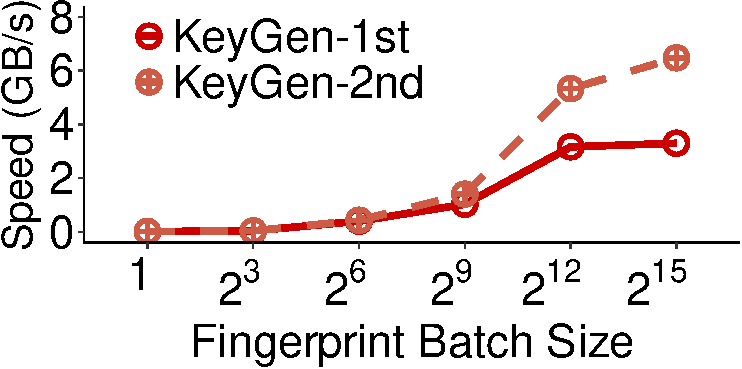
\includegraphics[width=0.48\textwidth]{pic/sgxdedup/expa2_keyEnclaveBatchSize_Performance_overall.pdf}                                         &
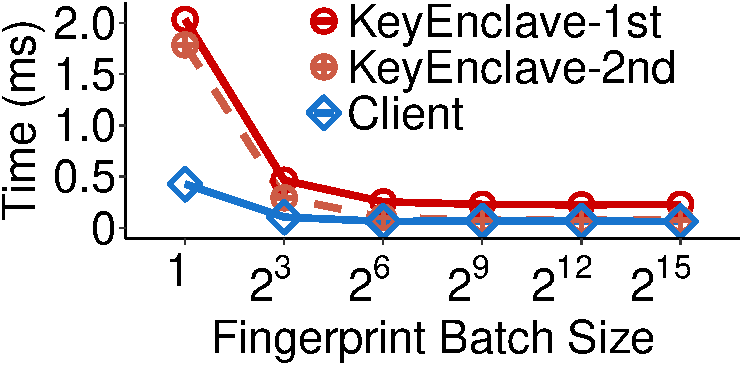
\includegraphics[width=0.48\textwidth]{pic/sgxdedup/expa2_keyEnclaveBatchSize_Performance_1st.pdf}                                               \\
\mbox{\parbox{0.48\textwidth}{\small (a) Key generation speed vs. fingerprint batch size}} &
\mbox{\parbox{0.48\textwidth}{\small (b) Computational time per generating 消息锁加密(MLE) keys of 1\,MB data}}
\end{tabular}
\caption{(Exp\#10) Impact of fingerprint batch size to key generation performance.}
\label{fig:exp-keygen-breakdown}
\end{figure}


\paragraph{Exp\#11 (Impact of ciphertext batch size).} 我们现在评估密文块批大小对 \sysnameS 的 PoW 性能的影响。与 Exp\#3 中考虑的计算 PoW 速度相反,我们测量 \textit{ 有效 PoW 速度},作为文件大小(即 2\,GB)与从 PoW enclave 开始的总时间的比率计算密文块的指纹,直到云验证所有指纹。我们禁用客户端的上传操作和云端的重复数据删除操作,以减轻性能噪音。

图~\ref{fig:exp-pow-impact}(a) 显示了有效 PoW 速度与不同批量大小的关系。我们看到有效 PoW 速度随着密文批量大小从 6.2\,MB/s 到 360.9\,MB/s 的增加而增加。图~\ref{fig:exp-pow-impact}(b) 显示了 PoW 安全区和云在 PoW 中每次操作 1\,MB 数据时的相应计算时间。云的消耗时间很低(例如,低于 0.05\,ms),而 PoW enclave 的时间随着批量大小从 4.1\,ms 减少到 2.7\,ms,因为减少了上下文切换开销(见 Exp \#10)。请注意,即使批量密文块的总大小超过 EPC 大小,PoW enclave 仍保持高计算性能,因为它不需要将数据内容复制到 enclave (\S\ref{sec:implementation})。

\begin{figure}[t]
\centering
\begin{tabular}{@{\ }c@{\ }c}
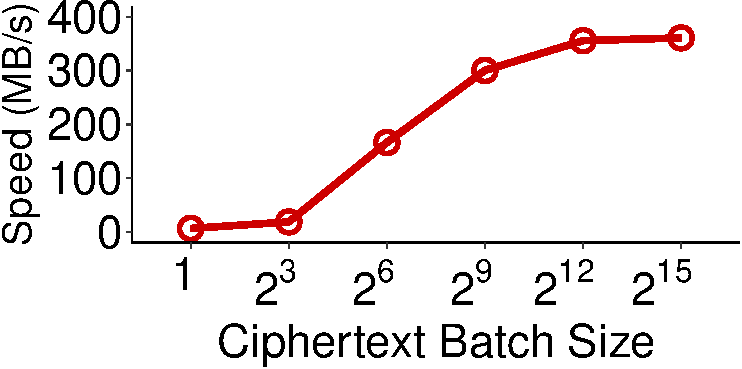
\includegraphics[width=0.48\textwidth]{pic/sgxdedup/expa4_powBatchSize_overall.pdf} &
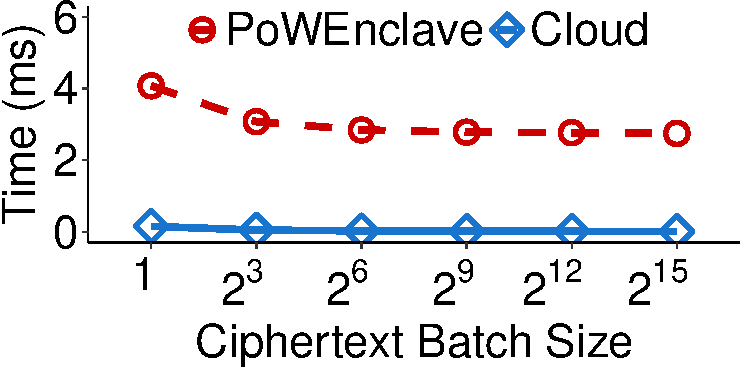
\includegraphics[width=0.48\textwidth]{pic/sgxdedup/expa4_powBatchSize_breakdown.pdf}                 \\
\mbox{\parbox{0.48\textwidth}{\small (a) Effective PoW speed vs. ciphertext batch size
}}                                                                 &
\mbox{\parbox{0.48\textwidth}{\small (b) Computational time per processing 1\,MB data}}
\end{tabular}
\caption{(Exp\#11) Impact of ciphertext batch size to PoW performance.}
\label{fig:exp-pow-impact}
\end{figure}


\paragraph{Exp\#12(密钥更新延迟)。} 回想一下,密钥安全区和云通过密钥回归独立地执行密钥更新,方法是从旧状态(\S\ref{subsec:key-management})导出新密钥状态。我们评估密钥安全区和云中的密钥更新延迟。

图~\ref{fig:rekeyingLatency}(a) 显示了 \textit{ first} 更新密钥操作的延迟与密钥回归参数(即,可承受的最大更新密钥次数(\S\ref{subsec:key-management }))。密钥安全区和云的密钥更新延迟随着密钥回归参数的增加而增加,因为更大的密钥回归参数意味着密钥更新的哈希计算更多。由于 SGX enclave 处理密集计算 \cite{harnik18} 的能力较弱,因此密钥 enclave 的密钥更新延迟大约比云高 1.22-1.56$\times$。

图~\ref{fig:rekeyingLatency}(b) 显示了每个rekeying操作的延迟,而关键回归参数固定为2$^{20}$。随着执行更多的密钥更新操作,密钥更新延迟会减少,因为每个密钥更新操作通过一次散列计算降低了后续密钥更新操作的计算复杂度。平均而言,密钥安全区的密钥更新延迟为 0.040\,s。相比之下,云的约为 0.027\,s,这意味着密钥更新开销是有限的。

\begin{figure}[t]
\centering
\begin{tabular}{@{\ }c@{\ }c}
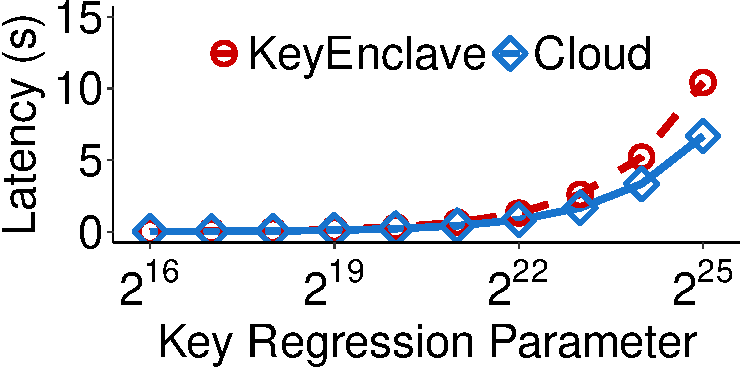
\includegraphics[width=0.48\textwidth]{pic/sgxdedup/expa5_keyRegression_time.pdf} &
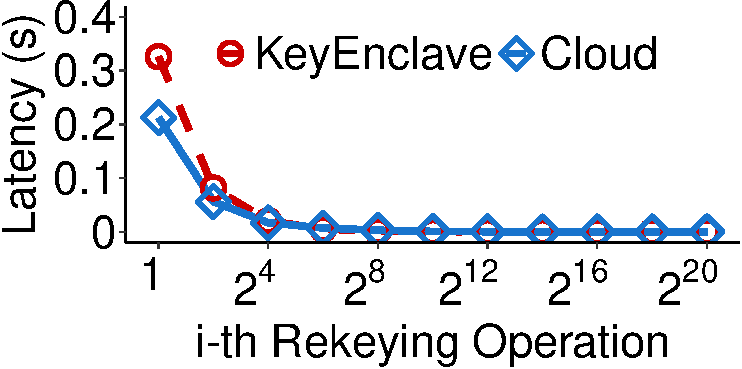
\includegraphics[width=0.48\textwidth]{pic/sgxdedup/expa5_keyRegression_time_default.pdf} \\
\mbox{\small (a) For different parameters} &
\mbox{\small (b) For different occurrences}
\end{tabular}
\caption{(Exp\#12) Rekeying latencies.}
\label{fig:rekeyingLatency}
\end{figure}

\subsection{对实际工作负载的评估}
\label{subsec:sgxdedup-real-world}

本文使用真实世界的工作负载(包含重复)评估 \sysnameS。本文在评估中考虑了两个真实世界的数据集。
\begin{itemize}[leftmargin=*]
\item 第一个数据集,称为 \textit{ FSL},包含来自文件系统和存储实验室 (FSL) \cite{fsl,sun16} 的共享文件系统的用户主目录的备份快照。每个快照列出了平均块大小为 8\,KB 的块的 48 位指纹。本文选择了 2013 年 1 月 22 日至 6 月 17 日的所有快照(在 \texttt{fslhomes} 下),总共覆盖了 56.2\,TB 的预重复数据删除数据。重复数据删除后数据集减少到 431.9\,GB(即 133.2$\times$ 的重复数据删除率)。
\item 第二个数据集,称为 \textit{ MS},包含来自 Microsoft \cite{meyer2011deduplication} 的 Windows 文件系统快照。每个快照列出了平均块大小为 8\,KB 的块的 40 位指纹。本文从原来的 857 个快照中抽取了 140 个快照,每个快照的大小约为 100GB。本文的数据集包含 14.4 TB 的预重复数据删除数据。重复数据删除后,它减少到 2.4\,TB(即 6$\times$ 的重复数据删除率)。
\end{itemize}



\paragraph*{Exp\#8 (Trace-driven performance).} 本文对\sysnameS 的上传和下载性能进行了trace-driven 评估。本文从 FSL 和 MS 中分别选择了 10 个快照,如下所示。对于 FSL,本文选择来自同一用户的快照具有较高的跨快照冗余;对于 MS,本文选择具有最多快照内冗余的快照。选择的 FSL 和 MS 快照分别采用 1.3\,TB 和 1.0\,TB 的预重复数据删除数据。由于本文的快照只包含没有实际数据的指纹,本文通过重复将其指纹写入备用块直到达到指定的块大小来重构每个明文数据块,因此相同(不同)指纹返回相同(不同)块。本文使用单个客户端一张一张地上传快照,然后以相同的上传顺序下载它们。本文将 \sysnameS 与 PlainDedup (Exp\#4) 进行比较。

\begin{figure}[t]
  \centering
  \begin{tabular}{@{\ }c@{\ }c}
  \multicolumn{2}{c}{
\includegraphics[width=0.9\textwidth]{pic/sgxdedup/expb2_trace_legend.pdf}} \\
  \hspace{-0.1in}
  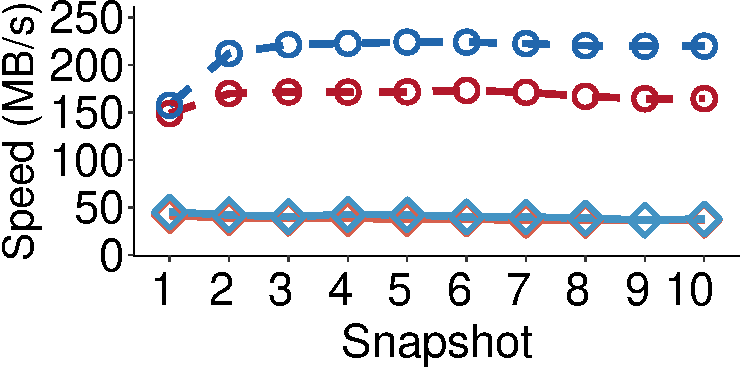
\includegraphics[width=0.47\textwidth]{pic/sgxdedup/expb2_trace_fsl_plain_sgx.pdf} &
  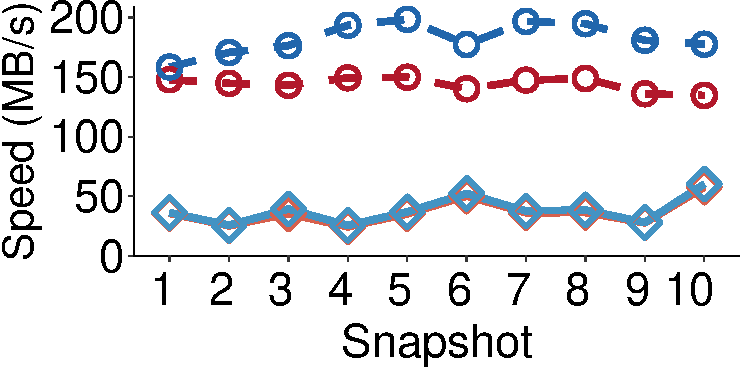
\includegraphics[width=0.47\textwidth]{pic/sgxdedup/expb2_trace_ms_plain_sgx.pdf}
  \vspace{-3pt}\\
  \mbox{\small (a) FSL dataset} &
  \mbox{\small (b) MS dataset}
  \end{tabular}
  \vspace{-6pt}
  \caption{(Exp\#8) Trace-driven upload and download performance.}
  \label{fig:sgxdedup-tracePerformance}
\end{figure}

图~\ref{fig:sgxdedup-tracePerformance}(a) 显示了跨 FSL 快照的上传和下载速度。 \sysnameS 和 PlainDedup 都实现了很高的上传速度,尤其是在第一个快照(例如 148.8\,MB/s \sysnameS 为 ,PlainDedup 为 157.5\,MB/s)。原因是 FSL 数据集跨快照的冗余度很高,两个系统都可以为后续快照上传较少的数据。与 PlainDedup 相比,\sysnameS 平均会导致上传性能下降 22.0\%。请注意,在本文使用随机工作负载的性能评估 (Exp\#4) 中,开销略大于 (17.5-21.4\%)。原因是现在在跟踪驱动评估中禁用了分块,\sysnameS 的瓶颈切换到 PoW(参见表~\ref{tab:sgxdedup-system-breakdown}),而 PlainDedup 的瓶颈是指纹。 \sysnameS 的下载速度从 41.3\,MB/s 下降到 36.4\,MB/s,PlainDedup 的下载速度从 45.0\,MB/s 下降到 37.9\,MB/s,主要是由于块碎片 \cite{lillibridge13} .本文可以通过重写和缓存 \cite{lillibridge13,cao2018ALACC} 来减轻块碎片。

图~\ref{fig:sgxdedup-tracePerformance}(b) 显示了跨 MS 快照的上传和下载速度。这两个系统的上传速度都低于 FSL 数据集,因为 MS 数据集有更多的非重复块(例如,MS 为 28.7\,M 而 FSL 为 18.3\,M)并加重了指纹索引的访问开销。与 PlainDedup 相比,\sysnameS 平均会导致 21\% 的上传速度下降。请注意,下载速度会波动(例如,\sysnameS 为 24.3-57.5\,MB/s,PlainDedup 为 25.6-60.3\,MB/s),因为某些 MS 快照具有更多非重复块,并且可能存储在可以通过顺序读取快速访问的连续区域(即更少的块碎片 \cite{lillibridge13})。

\paragraph*{Exp\#9(节省带宽)。} 本文评估 \sysnameS 的带宽效率。本文考虑使用源端重复数据删除(即客户端执行重复数据删除并仅将非重复的密文数据块上传到云)和基于存储目标的重复数据删除(即客户端上传所有密文数据块到云,对收到的密文数据块执行重复数据删除):(i)\textit{ 两阶段重复数据删除} \cite{li15},对单个用户应用源端重复数据删除,然后跨用户应用基于存储目标的重复数据删除; (ii) \textit{ 随机阈值重复数据删除} \cite{harnik2010side},它基于随机选择的阈值执行源端重复数据删除或基于存储目标的重复数据删除。本文在随机阈值重复数据删除中选择阈值的上限和下限分别为 20 和 2,如 \cite{harnik2010side}。对于FSL,本文聚合不同用户的当天快照,并将每个聚合快照按照创建时间的顺序添加到存储中。对于 MS,本文根据其快照 ID 添加每个快照(本文假设每个 MS 快照来自不同的用户)。本文将 \textit{ 带宽节省} 衡量为与预重复数据删除数据相比传输中数据减少的比例。在这里,本文不考虑元数据导致的带宽开销。

图~\ref{fig:sgxdedup-uploadTraffic} 显示了上传每个快照后的累积带宽节省。上传所有快照后,\sysnameS 在 FSL 和 MS 中分别实现了 99.2\% 和 83.2\% 的带宽节省。由于 \sysnameS 执行源端重复数据删除,因此其带宽节省也转化为存储节省。两阶段重复数据删除与 FSL 中的 \sysnameS 节省的带宽几乎相同,因为 FSL 数据集包含大量用户内冗余。另一方面,在 MS 中,两级重复数据删除仅节省了 47.9\% 的带宽(比 \sysnameS 少了 35.3\% 的绝对差异)。随机阈值重复数据删除具有不同的带宽节省,在 MS 中节省了 48.5\%,但在 FSL 中只有 7.8\%(小于 \sysnameS,绝对差异分别为 34.7\% 和 91.4\%)。

\begin{figure}[t]
\centering
\begin{tabular}{@{\ }c@{\ }c}
\multicolumn{2}{c}{
\includegraphics[width=0.9\textwidth]{pic/sgxdedup/upload_traffic_legend.pdf}} \\
\hspace{-0.1in}
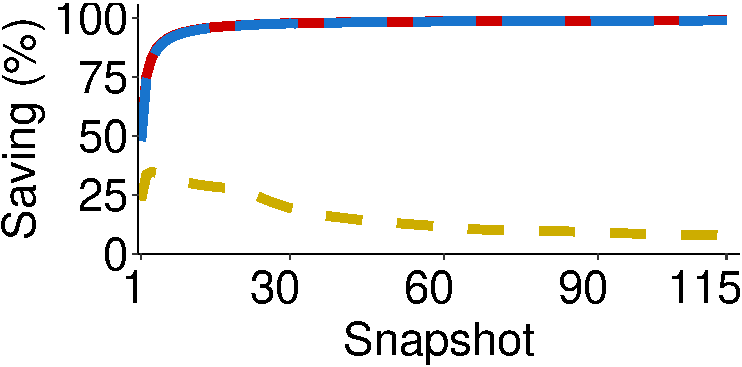
\includegraphics[width=0.47\textwidth]{pic/sgxdedup/upload_traffic_fsl.pdf} &
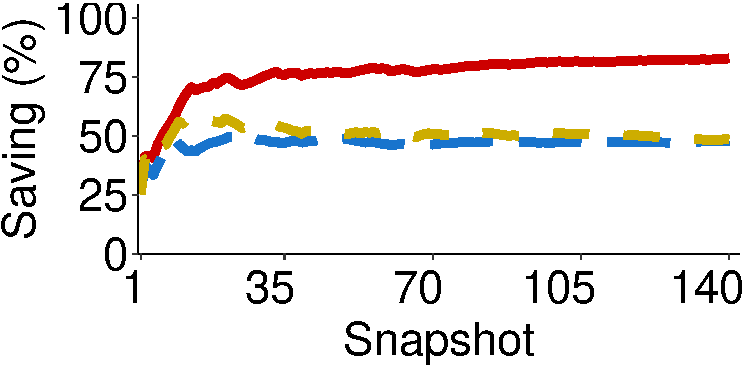
\includegraphics[width=0.47\textwidth]{pic/sgxdedup/upload_traffic_ms.pdf}
\vspace{-3pt}\\ 
\mbox{\small (a) FSL dataset} &
\mbox{\small (b) MS dataset}
\end{tabular}
\vspace{-6pt}
\caption{(Exp\#9) Cumulative bandwidth savings after each snapshot is stored.}
\label{fig:sgxdedup-uploadTraffic}
\end{figure}


\section{相关工作}
\label{sec:sgxdedup-related_work}

\noindent {\bf 消息锁加密(MLE) 密钥管理。} 基于 消息锁加密(MLE) 的传统 \cite{bellare2013MLE} 加密后重复数据删除系统(例如 \cite{adya2002farsite,cox2002pastiche,shah15})容易受到离线暴力攻击 \cite{bellare2013DupLESS}。 {\em DupLESS} \cite{bellare2013DupLESS} 建议服务器辅助 消息锁加密(MLE) 在专用密钥管理器中执行 消息锁加密(MLE) 密钥生成。服务器辅助 消息锁加密(MLE) 的后续研究集中在重复数据删除模式证明 \cite{armknecht2015transparent}、跨用户重复数据删除 \cite{zhou2015secdep} 和 消息锁加密(MLE) 密钥更新 \cite{qin17}。

一些研究以降低重复数据删除效率 \cite{zhou2015secdep,qin17} 或削弱安全性 \cite{li2020Info} 为代价来减轻基于块的 消息锁加密(MLE) 密钥生成的开销。 \sysnameS 在性能上优于这些方法,同时保留了重复数据删除的有效性和安全性 (\S\ref{subsec:sgxdedup-synthetic})。其他一些 消息锁加密(MLE) 密钥生成方法包括基于阈值的密钥管理 \cite{duan2014distributed} 和分散式密钥管理 \cite{liu15},但它们建立在密码原语(例如,阈值签名 \cite{duan2014distributed} 和密码认证密钥交换\cite{liu15}) 理论证明但不容易实现。

\paragraph*{防御侧信道攻击。} 源端重复数据删除具有带宽效率,但容易受到侧信道攻击 \cite{harnik10}。先前的研究 \cite{harnik10, li15} 结合了源端重复数据删除和基于存储目标的重复数据删除来防御侧信道攻击,而 \sysnameS 通过纯粹执行源端重复数据删除(\S\ref{subsec:sgxdedup-real-world})并使用 PoW 来防止侧信道攻击。此外,\sysnameS 比基于 Merkle 树的 PoW (\S\ref{subsec:sgxdedup-synthetic}) 更有效。其他一些研究通过放松安全性来提高 PoW 的效率(例如,\cite{pietro12,xu2013weak}),而 \sysnameS 使用客户端 SGX 来保护 PoW 的安全性。

\paragraph*{SGX-based storage.} SGX \cite{sgx} 已被广泛用于保护存储系统。 PESOS \cite{krahn18} 使用 SGX 强制执行对象存储的访问策略。 OBLIVIATE \cite{ahmad2018OBLIVIATE} 增强了基于 SGX 的文件系统对特权侧信道攻击的安全性。 EnclaveDB \cite{priebe18} 和 ObliDB \cite{eskandarian19} 保护外包数据库免受 SGX 信息泄露。 NEXUS \cite{djoko2019NEXUS} 通过 SGX 对不受信任的云存储启用细粒度的访问控制。在性能方面,Harnik \textit{ et al.} \cite{harnik18} 提出了减轻 SGX 实现的性能开销的指南。 ShieldStore \cite{kim19} 实现特定于应用程序的数据管理以限制安全区内存使用。 SPEICHER \cite{bailleu2019SPEICHER} 是一个基于 SGX 的基于 LSM 的键值存储,具有高效的 I/O 操作。

以上所有研究均未考虑重复数据删除。 Dang \textit{ et al.} \cite{dang2017Privacy} 提出了基于代理的协议,用于带宽高效的加密后重复数据删除,但这些协议没有解决密钥生成性能开销,也没有实现。 SPEED \cite{cui2019SPEED} 利用重复数据删除来提高 SGX 计算的效率,但 \sysnameS 使用 SGX 提高了加密后重复数据删除的性能。其他研究使用云端安全区进行 PoW 验证 \cite{you2020Proofs} 和安全的基于文件的重复数据删除 \cite{fuhry20},而 \sysnameS 使用客户端安全区进行有效的 PoW 证明生成并支持更细粒度的块-基于重复数据删除。

\section{本章小结}
\label{sec:sgxdedup-sgxdedup-conclusion}

本章基于可信执行环境解决了加密重复数据删除中的性能问题。本文提出了\sysnameS,它实现了一组安全区内部调用以在安全区内执行敏感操作,从而在保持安全性的同时加速加密重复数据删除。\sysnameS 包含三项关键设计:(1)安全高效的安全区管理;(2)自更新的会话密钥管理;以及(3)用于减轻在线加解密开销的基于TEE的推测性加密。此外,本文的实验分析表明\sysnameS 在合成数据集和真实世界数据集作为工作负载的情况下具有远超现有基于密码学机制的加密重复数据删除的性能表现。


\chapter{基于可信执行环境(Intel SGX)对内容学习攻击的主动检测}

% \section{简介}
\label{sec:featurespy-intro}

现有加密后重复数据删除中的数据所有权证明机制不足以完全击败恶意客户端(参见\S\ref{subsubsec:intro-problem-security})。即使通过数据块级的所有权证明保护源端重复数据删除,攻击者仍可通过枚举可能的数据内容发起推测内容攻击(Learning-content attack)\cite{harnik2010side, zuo2018mitigating}。具体来说,攻击者先验的了解数据文件的大部分格式化内容(例如,工资单),并旨在识别其他客户端拥有的文件的私有部分(例如,工资单中的实际工资和奖金)。攻击者通过枚举私有内容的可能取值来伪造大量文件,并对每个文件执行源端重复数据删除,最终在某些文件无需上传任何数据块时推断目标私有信息的取值。

本文扩展了以前的研究\cite{harnik2010side, zuo2018mitigating},证明在实践中推测内容攻击的严重性。具体来说,通过一个案例研究(参见\S\ref{sec:featurespy-attack}),本文说明针对具有较低信息熵(例如,包含数千个枚举取值)的文件,推测内容攻击可在本地局域网络环境中以不超过2分钟的时间开销完成攻击,而在真实云环境下也仅需8分钟左右完成。本文认为数据所有权证明无法阻止推测内容攻击,因为攻击者可以访问伪造文件的全部内容并且能向云服务端证明其对这些文件的所有权。

本章提出了\sysnameF,它通过主动检测每个客户端中的推测内容攻击来增强加密后重复数据删除的安全性。本文研究发现发起推测内容攻击的客户端具有较短时间内处理大量相似数据块(来自大量伪造的文件)的行为特征,且这些相似数据块中的信息修改仅限于针对数据块内容的小范围修改。另一方面,本文的研究表明,正常工作负载(未发生推测内容攻击)中的连续数据块(可能一起处理)彼此之间存在显着差异。因此,\sysnameF 在客户端可信执行环境(参见\S\ref{sec:background-tee})中检查所处理数据块的相似性,若客户端在短时间内处理了大量相似数据块,则判定为推测内容攻击可能发生,最终实现针对恶意客户端的主动侦测。

\sysnameF 建立在本文提出的基于TEE的数据所有权证明(参见\S\ref{chapter:sgxdedup})方案的基础之上,该方案可确保重复数据删除仅发生在经过安全区处理的加密数据块上。\sysnameF 基于加密数据块检测相似性,并将检测过程与安全区中的数据所有权证明耦合,以防止恶意客户端绕过检测过程。具体来说,\sysnameF 提出了相似性保留加密(similarity-preserving
encryption, SPE),相似性保留加密为消息锁加密增加了加密后数据的相似性保留能力,除了消息锁加密密钥,其额外根据原始数据的内容特征推导出特征密钥(feature key)。由于相似的原始数据很可能具有相同的特征密钥,相似性保留加密使用特征密钥加密一小部分原始内容(称为指标(Indicator))以保留相似性,并使用消息锁加密方案加密剩余的大部分内容以确保数据安全性。由于相似数据仅在少数区域不同,\sysnameF 通过比较使用特征密钥加密的小部分来检测原始数据是否相似。

本章实验分析表明\sysnameF 可以有效地检测推测内容攻击(例如,在本文的案例研究中,检测率最低为98.6\%),而产生误判的概率很低(例如,\sysnameF 的默认配置条件下为误判率为零)。此外,本文将\sysnameF 部署到基于TEE的高性能加密重复数据删除系统\sysnameS 中(关于\sysnameS 的相关设计参见\S\ref{chapter:sgxdedup}),以提高其应对推测内容攻击的安全性。本章提出的\sysnameF 的原型实现(即\prototype)相较于\sysnameS 增加的额外性能开销在基于真实世界数据集的性能测试中低至8.8\%(上传)和0.8\%(下载)。
% \section{推测内容攻击}
\label{sec:featurespy-attack}

除了伪造所有权攻击(参见\S\ref{subsec:background-encrypted-deduplication-pow}),源端加密后重复数据删除还面临另一种侧信道攻击(仍然由恶意客户端发起),称为推测内容攻击({\em learning-content attack})\cite{harnik2010side, zuo2018mitigating},它利用了源端重复数据删除泄露的重复数据删除结果(即,数据块是否已由任何其他客户端上传)。推测内容攻击假设攻击者先验地知道某些受害客户端拥有某个文件,其内容遵循公开的内容模板(即文件大部分内容已知)。攻击者的目标是识别文件中的私有部分。具体来说,攻击者会枚举私有部分的所有可能值,并生成许多伪造的文件(每个文件包含一种可能的值)。攻击者上传每个伪造的文件,如果被告知不需要传输某个文件的任意数据块(即伪造的文件不包含任何未被上传的数据块),则推断目标文件与当前伪造的文件相同。

本文认为数据所有权证明\cite{halevi11}(参见\S\ref{subsec:background-encrypted-deduplication-pow})不足以防范推测内容攻击,因为攻击者枚举了数据块的全部内容并且能够说服云服务端其对这些数据块的所有权。换句话说,数据所有权证明无法检测到这些数据块是完全由客户真实拥有的还是刻意伪造的。

\paragraph*{案例研究。}
本文扩展现有工作\cite{harnik2010side,zuo2018mitigating}对推测内容攻击的场景分析,设计案例验证推测内容攻击的可行性。考虑Alice和Bob为应届毕业学生,同时收到某公司的雇佣合同。他们将各自合同备份至云服务端。假设Alice为攻击者,通过推测内容攻击推断Bob合同中的薪水和签字费。

\begin{table}[!htb]
    \small
    \centering
    \begin{tabular}{@{}cccc@{}}
    \toprule
    测试环境 & 上传次数                            & 上传流量(MiB)                       & 攻击时间(秒)        \\ \midrule
    局域网  & \multirow{2}{*}{841.0 $\pm$ 608.3} & \multirow{2}{*}{7.4 $\pm$ 5.4} & 105.0 $\pm$ 76.1 \\
    阿里云  &                                 &                                 & 475.5 $\pm$ 339.8 \\
    \bottomrule
    \end{tabular}
    \caption{推测内容攻击开销:以上结果包含十次测试的平均值和基于T分布(Student's t-Distribution)的95\%置信区间}
    \label{tab:LRI-verify}
\end{table}

为了实现以上推测内容攻击案例,本文基于Google合同模版\cite{GoogleOffer},更改其中姓名、年薪(假设为6K的倍数\cite{harnik2010side},介于204K和804K之间)和签字费(假设为10K的倍数,介于300K和600K之间)以生成Alice和Bob的合同,每个合同约占18.5KiB。本文随机生成Bob的薪水和签字费,并通过基于图~\ref{fig:Cloud-based-encrypted-deduplication-storage-logic}设计实现的基础原型将Bob的合同存储至服务端。令Alice基于自身合同作为内容模版,枚举Bob所有可能的薪水和签字费,以实施推测内容攻击。本文分别在本地局域网(客户端、密钥服务器和服务端均部署在本地测试平台中,请参阅\S\ref{subsec:featurespy-evaluation-performance}以了解测试平台详细配置)和阿里云(将客户端和密钥服务器部署在本地测试平台并将云服务端部署在阿里云\cite{Alibaba},请参阅 \S\ref{subsec:featurespy-evaluation-performance}以了解测试环境详细配置)实现上述攻击。如表~\ref{tab:LRI-verify}所示,Alice需上传大约841份伪造合同,消耗7.4MiB网络流量(包括传输非重复密文数据块和元数据),在本地局域网和阿里云环境中推断Bob的隐私信息分别只需105.0秒和475.5秒。

\section{场景及假设}
\label{sec:featurespy-setting}
本文提出 \sysnameF 通过在客户端 {\em 可信执行环境 (TEE)} 中通过 {\em 主动检测学习内容攻击} 来增强加密后重复数据删除,从而完全击败恶意客户端。

\paragraph*{Trusted execution.} 本文建立在 {\em Intel Software Guarded Extensions (SGX)} \cite{sgx} 上来实现 TEE,因为 SGX 得到了当今商品计算机的广泛支持。除了 SGX,本文的设计 (\S\ref{sec:featurespy-design}) 可以扩展到其他支持 TEE 的可信计算技术 \cite{AMDSEV, pinto19}。

SGX 使用一组与安全相关的指令扩展 Intel CPU 以实现 TEE。它在硬件保护的内存区域(称为 {\em 安全区页面缓存 (EPC)})中分配一个 {\em 安全区},以便在具有机密性和完整性保证的情况下托管(in-enclave)内容。创建安全区后,SGX 提供 {\em 远程认证} 以通过远程实体(例如,云)对安全区进行身份验证,以及 {\em 安全密封} 在(经过身份验证的)enclave 和云端。此外,SGX 为安全区和未受保护的内存之间的交互提供了两个接口。程序可以通过 {\em 安全区调用 (ECalls)} 进入安全区执行安全区内部函数。在 ECall 中,它可以暂时退出安全区并通过 {\em 安全区外部调用 (OCalls)} 在不受保护的内存中调用不受信任的函数。



\paragraph*{部署场景。}图~\ref{fig:featurespy-model}展示了加密后重复数据删除的场景(\S\ref{subsec:featurespy-basics})。为了部署 \sysnameF,本文首先将安全区代码编译成共享对象 \cite{sgx},并将共享对象连同用于完整性验证的签名分发给每个客户端。云托管共享对象以验证每个客户端的安全区。具体来说,客户端初始化\sysnameF,通过加载共享对象创建对应的enclave,云端通过远程证明\cite{sgx}对每个enclave进行认证,以确保将正确的代码加载到enclave中。

在上传过程中,\sysnameF 处理明文数据块(由客户端生成),并为源端重复数据删除计算相应的密文数据块和指纹。未受损的客户端仅将不重复的密文数据块传输到云,而 \sysnameF 如果客户端被捕获以发起学习内容攻击,则会报告恶意客户端。

\begin{figure}
    \centering
    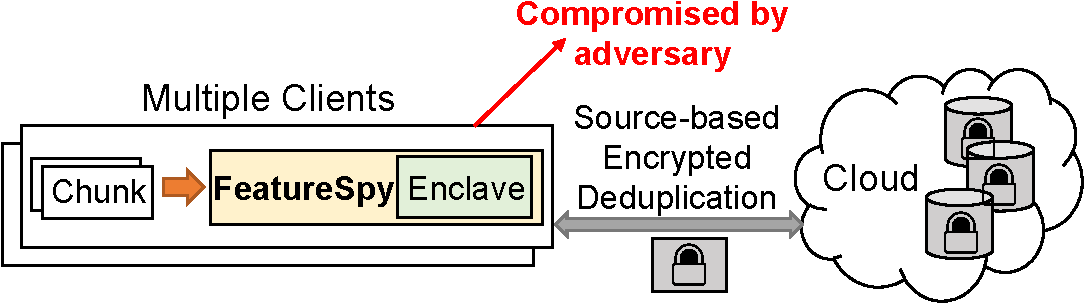
\includegraphics[width=\textwidth]{pic/featurespy/deployment.pdf}
    \vspace{-6pt}
    \caption{部署 \sysnameF.}
    \label{fig:featurespy-model}
    \vspace{-6pt}
\end{figure}

\paragraph*{威胁模型。} 本文的主要安全目标是增强加密后重复数据删除 (\S\ref{subsec:featurespy-basics}) 以防止 {\em 恶意} 客户端的安全性。与加密后重复数据删除 \cite{bellare2013MLE} 一样,本文考虑了一个旨在从任何存储的密文数据块中窃听原始内容的受损云。此外,本文考虑一个恶意客户端,旨在学习其他未受损客户端的原始明文数据块。具体来说,恶意客户端可以访问其受损的明文数据块和密钥,并任意伪造新的明文数据块以发起学习内容攻击(\S\ref{subsec:featurespy-basics})。此外,它可以篡改未受保护的内存中的内容和操作,以逃避 \sysnameF 的捕获。

本文的威胁模型做出以下假设。
\begin{itemize}[leftmargin=*]
    \item
          每个客户端与云之间的通信通道受 SSL/TLS 保护以防窃听。
    \item
          SGX安全区是受信任和经过身份验证的(例如,在首次引导时通过远程证明),以便诚实地执行攻击检测以防止篡改。此外,与之前的作品 \cite{shinde20, ren21} 一样,SGX安全区只为加密密钥(即 \S\ref{sec:featurespy-implementation} 中的证明密钥)而不是所有安全区内的内容保留机密性;鉴于针对 SGX 的侧信道攻击,这一点很重要(例如,请参阅 \cite{fei21} 进行调查)。
    \item
          恶意云可能会破坏外包数据以损害完整性。 \sysnameF 没有解决威胁,但它与 \textit{  (proof data prosession,PDP)} \cite{ateniese2007provable} 和 \textit{  (proof of retrievability,PoR)} \cite{juels07} 兼容,以执行定期的完整性验证外包数据,以及容错存储,以从损坏 \cite{li15} 中恢复数据。
\end{itemize}
\section{FeatureSpy设计}
\label{sec:featurespy-design}
我们在设计 \sysnameF 时考虑了以下目标。

\begin{itemize}[leftmargin=*]
\item {\bf 攻击检测。} 它可靠地检测学习内容攻击以防止客户端篡改(即鲁棒性)。此外,它实现了捕获攻击的高概率,而误判的数量很少。
\item {\bf 保密性和带宽/存储效率。} 保留基于数据源的加密重复数据删除,从而达到数据保密性和带宽/存储效率。此外,它还减轻了由于密钥泄露导致的信息泄露。
\item {\bf 低性能开销。} 它检测写入路径中的学习内容攻击,并在加密重复数据删除部署中产生低性能开销。
\item {\bf 有限可信计算库 (TCB)。} 它管理 SGX安全区的最小信任部分和函数调用接口;鉴于滥用接口函数调用 \cite{lie05},这是一个必要的设计目标。
\end{itemize}

我们首先提出一个稻草人(不安全)设计来演示我们如何通过监控内容处理来检测学习内容攻击。然后,我们提出 \sysnameF,它可以防止恶意客户端绕过攻击检测程序。


\subsection{原型设计}
\label{subsec:featurespy-basic}
\paragraph*{Overview.} 我们的见解是,发起学习内容攻击的对手枚举了许多 {\em similar} 块,这些块遵循相同的内容模式,并在几个区域发生信息变化。换句话说,这样的块很可能共享相同的 {\em 内容特征}(可以基于相应的块内容通过 {\em N-transform} \cite{shilane12} 生成,参见后面的部分 “features本小节的提取”),并在一个小的时间窗口内进行处理。这导致攻击过程中每个时间窗口的{\em skew feature distribution},因为一些特征被一起处理的大多数块共享。

另一方面,我们认为在实际未篡改的存储工作负载中,连续块(一起处理 \cite{zhu08})的特征分布通常是 {\em uniform}(即,不同的特征对应于相同数量的块)。具体来说,我们分析了两个真实世界的数据集(有关数据集的详细信息,请参阅 \S\ref{subsec:featurespy-datasets}),并将每个数据集中的块流划分为多个不重叠的窗口,这样每个窗口都包含 $W$ 连续块。我们通过 N 变换 \cite{shilane12} 为每个块提取三个有序特征。对于每个窗口,我们计算共享相同第 i 个特征($ i=1、2$ 和 $3$)。窗口的归一化差值越小,表示对应的特征分布越均匀。


图~\ref{fig:featurespy-featureDistribution} 展示了所有窗口(大小分别为 $W$ = 1\,K, 5\,K, 和 10\,K)基于它们的第一个特征(即, $i$ = 1)。其他特征的结果是相似的,因为不同阶的特征不太可能相同(由于 N 变换原理);因此我们在这里省略它们。我们观察到,尽管不同窗口之间的归一化差异分布是倾斜的,但每个窗口只有一个小的归一化差异值(例如,Linux 中高达 0.035,CouchDB 中高达 0.005)。当$W$ = 1\,K, 5\,K 和 10\,K 时,91.5\%、58.3\% 和 29.9\% 的特征甚至被相同数量的块共享(即均匀特征分布) CouchDB 窗口,分别。

\begin{figure}
  \centering
  \begin{tabular}{cc}
    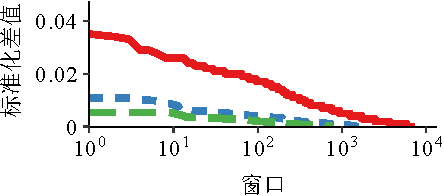
\includegraphics[width=0.45\textwidth]{pic/featurespy/plot/featureDistribution/featureDistributionLinux.pdf} &
    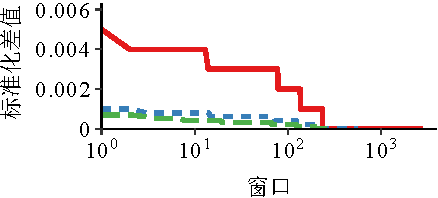
\includegraphics[width=0.45\textwidth]{pic/featurespy/plot/featureDistribution/featureDistributionCouchbase.pdf} \\
    {\small (a) Linux} & {\small (b) CouchDB} \\
    \end{tabular}
  \vspace{-6pt}
  \caption{两个真实数据集中不同窗口的标准化差异。 x 轴上的窗口按它们的归一化差异排序。}
  \label{fig:featurespy-featureDistribution}
  \vspace{-6pt}
\end{figure}

因此,稻草人设计通过 {\em 区分特征分布} 来检测学习内容攻击。图~\ref{fig:featurespy-architecture-strawman} 展示了稻草人设计的架构工作流程。由于 \sysnameF 与可能篡改未受保护内存的客户端位于同一位置,因此它通过 SGX安全区保护特征提取和攻击检测程序,从而诚实地报告攻击事件。具体来说,它进入安全区以提取每个明文块的内容特征,如果许多块匹配相同的内容特征(即相似),则报告攻击。如果没有宣布攻击,它将继续执行基于数据源的加密重复数据删除 (\S\ref{subsec:featurespy-basics})。在下文中,我们将讨论设计细节。


\paragraph*{特征提取。}
我们通过 {\em N-transform} \cite{shilane12} 提取每个明文块的内容特征,这被广泛用于检测块级相似性。 N-transform 是基于 $N$(例如,默认为 12)对系数 $(a_i, m_i)$ 定义的,其中 $N$ 表示有多少 {\em sub-features}(基于 N-transform 生成的特征,见下文)为每个块提取。具体来说,对于每个明文块 $M$,它使用 Rabin 指纹 \cite{rabin81} 在块数据的 32 字节滑动窗口上计算许多指纹,并将每个滑动窗口中的 Rabin 指纹 $fp$ 转换为:
\begin{eqnarray}
  \label{eq:featurespy-feature}
  \pi_i = a_i * fp + m_i \mod 2^{32},
\end{eqnarray}
其中$i$ = 1, 2,\ldots, $N$。如果在其他 Rabin 指纹中,$fp$ 导致 {\em 最大值} $\pi_i$,则它将 $M$ 的第 $i$ 个子特征导出为 $fp$。基本原理是小区域的变化可能会影响一些 Rabin 指纹,其中只有少数(作为子特征)产生 $\{\pi_i\}$ 的最大值。因此,对于类似的块,大多数子特征保持稳定。

N-transform 通过将多个(例如,默认情况下为四个)连续的子特征组合在一起来计算一个特征。它通过一组特征 $S$(例如,默认情况下特征数量 $|S| = 3$)来表征每个块,以减轻比较许多子特征以进行相似性检测的计算开销。具体来说,两个块的共同特征越多,它们就越有可能相似。


\paragraph*{攻击检测。}
我们在安全区中管理一个哈希表来跟踪有多少明文块共享相同的内容特征。哈希表的每个条目将一个特征映射到该特征在不同块中出现的次数(四个字节)。此外,我们定义了一个窗口大小 $W$(例如,默认为 5\,K)并定期清除每个处理 $W$ 块的所有表条目,这样哈希表只保留 {\em 最近} 出现的特征短时间内。请注意,哈希表最多为 5\,K $\times$ 3 $\times$ (16 bytes + 4 bytes) $\approx$ 300\,KiB 并为 SGX安全区添加了可忽略的内存开销,其中每个块都有三个特征,每个特征由四个子特征拼接而成,每个子特征根据 N-transform 的默认配置占用四个字节。

为了检查每个明文块,我们根据其内容特征查询哈希表。如果一个特征不存在,我们将这个特征添加到哈希表中,并用一个初始化对应的出现;否则,如果该特征存在,我们将相应的出现加一。如果发生达到窗口大小 $W$ 的预定义比率 $T$(例如,默认情况下为 3\%),我们将报告攻击。



\subsection{FeatureSpy概览}
\label{subsec:featurespy-secure_design}

稻草人设计的一个安全限制是它容易{\em 绕过}攻击检测程序(图~\ref{fig:featurespy-architecture-strawman})。 具体来说,恶意客户端可以直接注入其自构建的块以供未受保护的操作(例如,密钥生成)处理,以发起学习内容攻击(\S\ref{subsec:featurespy-basics})。


\begin{figure}
  \centering
  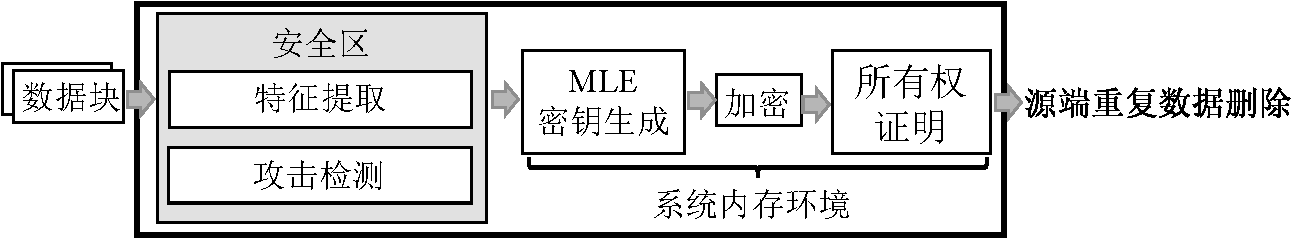
\includegraphics[width=\textwidth]{pic/featurespy/naive.pdf}
  \caption{Architectural workflows of \textit{Strawman design}. It is vulnerable to bypassing the detection procedure.}
  \label{fig:featurespy-architecture-strawman}
\end{figure}

\sysnameF 基于 {\em SGX-based PoW} \cite{ren21} 构建,以防止客户端逃避检测过程。具体来说,基于 SGX 的 PoW 方法 \cite{ren21} 将每个密文块作为输入并进入 SGX 安全区以计算密文块的指纹以及指纹的签名。只有当签名被成功验证时,云才会继续检查指纹是否对应于存储的密文块(即重复数据删除)。由于云根据 SGX安全区处理的 {\em authenticated} 指纹进行响应,因此客户端无法识别未经授权访问的块的存在。

因此,一种天真的方法是在稻草人设计中扩大 enclave,以在安全区中完全执行检测、密钥生成、加密和基于 SGX 的 PoW。在这种情况下,只有程序处理的块SGX安全区中的数据被云接受重复数据删除(由于基于 SGX 的 PoW),恶意客户端无法绕过任何程序。
然而,该方法会产生巨大的 TCB 并引入潜在的性能 \cite{arnautov16, harnik18, dinhngoc19} 和安全 \cite{lie05} 问题。

\begin{figure}
  \centering
  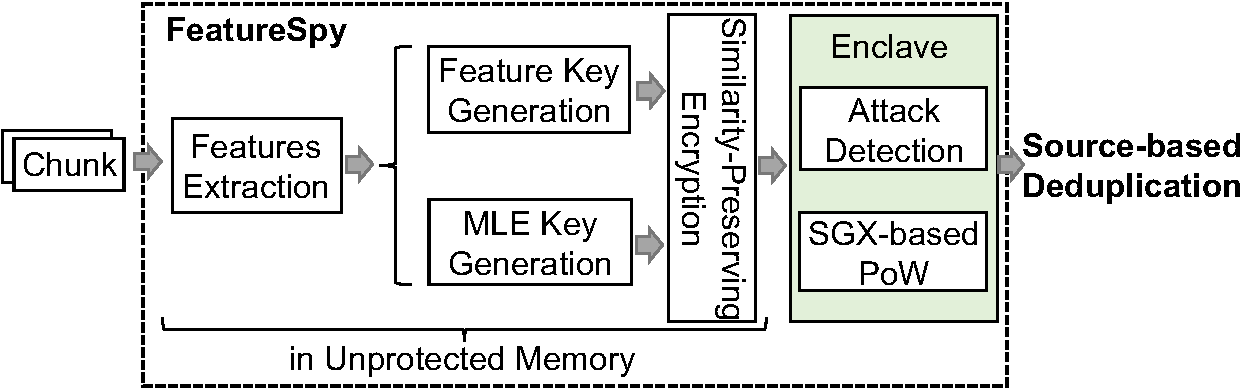
\includegraphics[width=\textwidth]{pic/featurespy/architecture.pdf}
  \caption{Architectural workflows of \textit{Secure design}. \sysnameF couples the attack detection procedure with SGX-based PoW \cite{ren21} in the enclave, in order to prevent the bypassing.}
  \label{fig:featurespy-architecture-secure}
\end{figure}

\sysnameF 提出{\em 进行基于密文块的攻击检测},并且只将检测过程与安全区中基于 SGX 的 PoW 耦合(图~\ref{fig:featurespy-architecture-secure}),以减少大小TCB 的。


\paragraph*{挑战。}
然而,{\em 基于密文块检测相似性} 提出了一个新的挑战,因为安全区现在只查看加密数据。在 MLE 之后检测相似性是不可能的,因为 MLE 密钥是从明文块 (\S\ref{subsec:featurespy-basics}) 的 {\em whole contents} 派生的。这会将相似(但不同)的明文块映射到完全不同的密文块,从而破坏相似性。

另一种加密原语是 {\em 基于特征的加密 (FBE)},它基于从每个明文块的内容特征派生的密钥(称为 {\em 特征密钥})执行加密/解密。由于相似的块仅在少数数据区域中有所不同,因此它们可能具有相同的特征密钥,以及前几个数据块(在 AES 中每个数据块占用 16 个字节)。考虑到加密重复数据删除 \cite{douceur02, shah15} 需要一个固定的 {\em 初始化向量 (IV)}(以保持确定性加密),FBE 保持了相似块的前几个数据块的相等性(由于 {\ em block-chaining encryption} 分组密码模式的属性,例如 {\em cipher block chaining (CBC)} 和 {\em cipher feedback (CFB)} \cite{dworkin01}),并且可以通过比较进行相似性检测每个密文块中的此类数据块。


然而,FBE 容易受到密钥泄露的影响,因为一个特征密钥对应于一组具有相同内容特征的块。恶意客户端可以使用其受损的功能密钥来完全解密许多块,甚至其中一些是 {\em 超出其访问范围}。


这给选择合适的密码原语带来了两难选择:MLE 对密钥泄露具有鲁棒性(即,泄露的 MLE 密钥不能用于解密除相应的块之外的其他块)但会破坏相似性,而 FBE 保留原始块的相似性但易受攻击关键妥协。

\subsection{相似性保留加密(SPE)}
\label{subsec:featurespy-spe}

我们提出了{\em 相似性保留加密 (SPE)},它同时建立在 MLE 密钥和特征密钥之上,以通过 MLE 密钥减轻密钥泄露,同时通过特征密钥保持相似性。具体来说,由于相似块的内容差异有限,SPE 从每个明文块中抽取一小部分(例如,前 32 个字节,占 8\,KiB 块的 0.4\%),称为 {\em similarity indicator} ,使得相似块的相似度指标很可能是相同的。它用相应的特征密钥加密每个明文块的相似性指标,而剩余的大部分(占 8\,KiB 块的 99.6\%)块内容用 MLE 密钥加密。然后,我们可以通过验证相应的(加密的)相似性指标(例如,每个密文块的前 32 个字节)是否相同来检测基于密文块的相似性。请注意,SPE 不会降低跨用户加密重复数据删除 (\S\ref{subsec:featurespy-basics}) 的存储效率,因为相同的块共享相同的内容特征(因此特征密钥)和 MLE 密钥。

我们认为 SPE 减轻了 FBE 针对密钥泄露的信息泄漏。洞察力是,受损块 $M$ 的特征密钥只能用于解密与 $M$ 相似的块的相似性指标。但是,由于此类块可能具有与 $M$ 相同的相似指标,因此 SPE 不会导致额外的信息泄漏。即使是稀有块(类似于 $M$)具有不同的相似性指标,与 FBE 相比,信息泄漏也大大减少,并受相似指标的大小影响。
在下文中,我们将介绍如何为 SPE 生成特征密钥的设计细节。


\paragraph*{功能密钥生成。}
回想一下,我们通过 N 变换(\S\ref{subsec:featurespy-basic})为每个明文块提取三个内容特征,一个基本的密钥生成方法(称为 {\tt allFeature})是连接所有特征,并计算基于连接结果的加密哈希的特征密钥。但是,{\tt allFeature} 无法为许多相似的块生成相同的特征键。具体来说,如果相似块的内容差异恰好在产生子特征(\S\ref{subsec:featurespy-basic})的滑动窗口中,则块将具有不同的特征键,并且无法检测到相似度即使剩余的原始内容相同。

我们基于 {\em 基于采样的方法} \cite{bhagwat09, dong11, qin17} 来放宽密钥生成标准。这个想法是为每个明文块采样一个{\em 代表}特征,并根据采样的特征计算特征密钥。这可以容忍内容差异,并为各种明文块生成相同的特征密钥。

我们考虑了两种选择代表性特征的方法。具体来说,{\tt firstFeature} 根据每个明文块的 {\em first} 特征生成特征密钥。优点是我们不需要计算后续的子特征和特征(\S\ref{subsec:featurespy-basic}),并减轻 N-transform 的计算开销 \cite{zhang19}。

我们还考虑 {\tt minFeature},它建立在 {\em Broder's theorem} \cite{broder97} 的基础上,根据每个的 {\em minimum} 特征(即在所有特征中具有最小值)生成特征键明文块。具体来说,布罗德定理指出,如果两个明文块具有许多共同特征(即,相似的概率很高),它们很可能共享相同的最小特征。那是:
\begin{eqnarray}
  \label{eq:featurespy-broder}
 \Pr[\min(S_1) = \min(S_2)] = \frac{|S_1 \cap S_2|}{|S_1 \cup S_2|},
\end{eqnarray}
其中 $S_i$ 是明文块 $M_i$ 的特征集合,$\min(S_i)$ 返回集合 $S_i$ ($i = 1, 2$) 中特征的最小值。因此,{\tt minFeature} 倾向于为高度相似的块生成相同的特征键。在 \S\ref{sec:featurespy-evaluation} 中,我们将研究 SPE 的不同密钥生成方法的权衡。

请注意,除了处理特征之外,另一种设计是基于第一个或最小 {\em sub-feature} 生成特征密钥。由于子特征的低熵,我们不选择这种设计。根据 N-transform 的原始配置 \cite{shilane12},每个子特征只有四个字节,攻击者可以通过枚举所有可能的子特征/密钥(最高 $2^{ 32}$)。另一方面,在 \S\ref{sec:featurespy-implementation} 中,我们重新配置 N-transform 以确保基于特征的密钥空间足够大(例如,$2^{256}$)以对抗暴力破解攻击。


\subsection{安全性分析}
\label{subsec:featurespy-security}
我们讨论了 \sysnameF 的机密性(特别是 SPE,它是底层加密原语),然后讨论了它对恶意客户端的鲁棒性。

\paragraph*{对受损云的保密性。}
我们已经讨论了 SPE 在密钥被泄露 (\S\ref{subsec:featurespy-spe}) 时相对于 FBE 的安全性改进,现在关注密钥保持安全的情况。我们的目标是证明 SPE 可以保护加密重复数据删除对受损云的安全性。具体来说,由于 SPE 通过 MLE 和 FBE 执行加密,因此其安全性降低到 MLE 和 FBE 的安全性。之前的工作 \cite{bellare13a} 表明,当明文块是从一个大的空间使得很难预测从空间中选择的任何块(即 {\em 不可预测})。在下文中,我们(非正式地)表明,如果特征不可预测,FBE 会保留 MLE 的安全性。


我们将 FBE 视为 MLE 的一种通用形式。如果我们将采样的特征(例如,{\tt firstFeature} 和 {\tt minFeature} 的代表特征,以及 {\tt allFeature} 的所有特征)视为消息 $M$,那么 FBE 实际上使用$M$的密码散列来加密对应的扩展$f(M)$(即明文块),其中$f(\cdot)$是一个扩展函数。由于每个 $M$ 都是不可预测的,因此密钥对多项式时间的对手保持机密。然后,如果底层对称加密是安全的,则对手无法区分密文和随机值。

请注意,我们的非正式分析依赖于特征不可预测的安全假设,而我们可以通过服务器辅助密钥生成 \cite{bellare13b} 来缓解不可预测的假设(请参阅 \S\ref{sec:featurespy-implementation} 了解我们如何部署 \ sysnameF 在解决不可预测假设的现有加密重复数据删除系统中)。


\paragraph*{对恶意客户端的鲁棒性。}
我们已经讨论过攻击者无法绕过检测程序(\S\ref{subsec:featurespy-secure_design}),现在关注对其他恶意行为的鲁棒性(\S\ref{sec:featurespy-setting})。


\begin{itemize}[leftmargin=*]
  \item {\bf 案例 1:篡改不受保护的程序。}
    \sysnameF 通过 SGX 保护检测程序,但恶意客户端可以篡改未受保护的程序。它可能会操纵特征、相似性指标和密钥,以欺骗 \sysnameF。
    我们认为,这些操作无助于从遵循我们设计的其他诚实客户那里学习内容,因为这些操作导致与 SPE(由诚实客户应用)产生的密文块不同,即使原始明文块是相同的。这个 {\em 禁止重复数据删除},依赖重复数据删除模式泄漏的学习内容攻击是不可能的。
  \item {\bf 案例2:篡改数据处理。}
    由于 \sysnameF 在每个处理窗口的粒度上监控数据相似性,恶意客户端可能会篡改正在处理的数据流,并小心地插入相似的块(用于攻击),使得每个窗口只包含一小部分相似的块.尽管 \sysnameF 在这种情况下无法检测到攻击,但我们认为它减缓了学习内容攻击。例如,在没有 \sysnameF 的情况下,恶意客户端可以用相似的块(即,数量为 $W$)填充每个窗口以进行攻击,但 \sysnameF 确保它可以提交最多 $W\times T$ 的相似块(否则会被检测到)。攻击成本降低$1/T$倍。通过配置一个小的$T$,我们可以使学习内容攻击成本太高而变得不切实际;权衡是增加了误判的可能性(即在正常情况下报告攻击)。
\end{itemize}
  
  
  
  \paragraph*{限制。}
  \sysnameF 检测来自每个 {\em 独立} 客户端的学习内容攻击。但是,攻击者可能会破坏多个客户端以合作发起学习内容攻击。现在每个客户端上传的相似块的数量大大减少,\sysnameF 可能无法有效检测到异常。我们将防御合作学习内容攻击作为我们未来的工作。
\section{实现}
\label{sec:featurespy-implementation}
我们使用 OpenSSL 1.1.1l \cite{openssl}、SGX SDK 2.15 \cite{sgxsdk} 和 SGX SSL \cite{sgxssl} 实现 \sysnameF,并将其部署到现有的基于 SGX 的加密后重复数据删除系统 {\em SGXDedup} \cite{ren21} 来提高其针对学习内容攻击的安全性。具体来说,SGXDedup除了每个客户端和云端之外,还维护一个{\em key server}来管理一个全局secret,并根据chunk指纹和全局secret生成每个明文chunk的MLE key,从而对 {\em 离线暴力攻击} 具有鲁棒性(即解决了不可预测的假设)\cite{bellare13b}。为了加速基于数据源的加密后重复数据删除,它在密钥服务器中部署了一个 SGX 安全区,并执行 {\em 推测性加密} \cite{eduardo19} 以减轻(服务器辅助)密钥生成的在线计算开销。此外,它还部署了一个客户端安全区来执行基于 SGX 的高效 PoW (\S\ref{subsec:featurespy-secure_design})。请注意,SGXDedup 无法抵御学习内容攻击(\S\ref{subsec:featurespy-attack}),我们的新原型(称为 \prototype)是为了增强 SGXDedup 以抵御学习内容攻击的安全性。目前,\prototype(包括底层的 SGXDedup)由 C++ 中的 16\,K LoC 组成。下面,我们重点介绍与 \prototype 相关的实现细节。


\paragraph*{设置。}
初始化后,\prototype 遵循 SGXDedup,通过 NIST P-256 椭圆曲线中的 {\em Diffie-Hellman 密钥交换 (DHKE)} 在云和每个客户端安全区之间共享一个 {\em proof key}。证明密钥在基于 SGX 的 PoW 中用于生成和验证签名(见下文)。


\paragraph*{密钥生成。}
\prototype 适用于通过 Rabin 指纹 \cite{rabin81} 生成的可变大小明文数据块,最小、平均和最大大小分别为 4\,KiB, 8\,KiB 和 16\,KiB。为了在特征键 (\S\ref{subsec:featurespy-spe}) 上提供足够的熵,它将滑动窗口大小和 N 变换中的模数分别配置为 64 字节和 $2^{64}$。它生成 12 个子特征(每个 8 个字节),并将四个子特征的串联散列以形成每个特征(32 个字节)。它根据来自密钥服务器(如 SGXDedup \cite{ren21})的每个明文数据块的指纹请求 MLE 密钥,以及基于采样特征的特征密钥(根据 {\tt firstFeature},{\ tt minFeature} 或 {\tt allFeature})。


\paragraph*{安全区操作。}
加密后(通过 AES-CFB-256 实现),\prototype 将 4,096 个密文数据块分批到安全区中进行处理,以减轻 SGX 上下文切换开销 \cite{arnautov16}。它跟踪哈希表中相似性指标的出现,并将窗口大小 $W$ 和比率阈值 $T$ 的默认值分别配置为 5\,K 和 3\%。

\prototype 遵循 SGXDedup 将源端重复数据删除与基于 SGX 的 PoW 相结合。它通过证明密钥基于 4,096 个指纹(密文数据块)的串联生成签名(通过 AES-CMAC 实现),以便云使用相同的密钥验证这些指纹的真实性。云通过LevelDB\cite{leveldb}实现指纹索引(\S\ref{subsec:featurespy-basics}),并通知客户端只传输非重复密文数据块。

\paragraph*{存储管理。}
云端以 8\,MiB {\em 容器} 为单位管理非重复密文数据块,以减轻磁盘 I/O 开销。对于每个文件,它管理一个 {\em file recipe},其中列出了密文数据块的指纹,以及相应的 MLE 密钥和特征密钥。为保护机密性,每个客户端在将其外包到云端之前,都会使用单独的主密钥对文件配方进行加密。

要下载文件,客户端首先从云端检索文件配方,并使用相应的主密钥对其进行解密。然后,客户端根据文件配方检索密文数据块,并根据 MLE 密钥和功能密钥对其进行解密。

\paragraph*{优化。}
我们应用标准方法来提高 \prototype 的性能。每个客户端在不同线程中提取多个明文数据块的内容特征,并在管道中并行处理分块、密钥生成、加密、PoW和上传。此外,为了提高下载性能,云会在内存中维护一个最近最少使用的缓存 (1\,GiB) 来保存最近恢复的容器。对于每个下载请求,它首先在缓存中搜索容器,并且仅当容器不在缓存中时才从磁盘中检索容器。
\section{实验分析}
\label{sec:featurespy-evaluation}


本文进行了广泛的评估来研究 \sysnameF (\S\ref{subsec:featurespy-evaluation-detection}) 的攻击检测有效性,以及 \prototype 在合成 (\S\ref{subsec:featurespy-syn}) 和现实世界中的性能(\S\ref{subsec:featurespy-real}) 工作负载。本文将主要结果总结如下:

\begin{itemize}[leftmargin=*]
\item \sysnameF 根据相应的密文数据块有效地找到相似的明文数据块。例如,当它们彼此进行中等修改时,它会检测到多达 80.2\% 的相似块。
\item \sysnameF 有效地检测到学习内容攻击,即使对手在普通内容快照中提交枚举内容。同时,它为现实世界的数据引入了低误判(例如,默认配置中的零)。
\item \prototype 在处理大规模真实世界数据时,在 SGXDedup(即没有 \sysnameF)的情况下会产生有限的上传(例如,8.8\%)和下载(例如,0.8\%)的性能开销。
\item 与现有的 \cite{harnik10, li15} 方法相比,可以安全抵御学习内容攻击,\prototype 具有带宽效率(例如,将网络流量节省高达 98.9\%)。
\end{itemize}


\subsection{数据集}
\label{subsec:featurespy-datasets}

\paragraph*{合成数据集。}

本文考虑三种类型的合成数据集进行评估。通过以受控方式修改基本块来生成第一数据集。具体来说,本文首先创建一个 8\,KiB 基本块 $M$。每次,本文在 $M$ 中随机选择 $x$ 个位置,并在每个位置更改 $y$ 个字节,以创建一个修改过的块。经过 10\,K 次修改后,本文得到一个合成数据集 {\em SYNChunk}$(x, y)$,其中包括从同一个基本块 $M$ 修改的 10\,K 个块。本文使用 SYNChunk$(x, y)$ 作为(相似块的)基本事实来研究相似性检测的有效性(Exp\#1 和 Exp\#2)。

此外,本文将 {\em SYNFile}$(x, y)$ 视为大小为 4\,KiB 的文件。本文假设 SYNFile$(x, y)$ 在文件内容中包含 $x$ 未知变量(其值将被推断),并且每个变量的值是从大小为 $y$ 的空间中选择的。本文使用 SYNFile$(x, y)$ 作为目标文件来研究 \sysnameF 在不同情况下的检测有效性(Exp\#4)。本文不考虑更大的目标文件,因为对手需要枚举更多相似的块(用于攻击)并且更有可能被 \sysnameF 捕获。

此外,本文将 {\em SYNUnique} 生成为一组 2\,GiB 文件,每个文件都包含全局非重复块。本文使用 SYNUnique 对 \prototype (\S\ref{subsec:featurespy-syn}) 的性能进行压力测试。

\paragraph*{Real-world datasets.} 本文考虑四个真实世界数据集,其特征总结在 Table~\ref{tab:featurespy-datasets} 中: (i) {\em FSL} \cite{fsl},其中包括 795 个 home 2013 年 1 月 22 日至 6 月 17 日 9 名学生的目录快照; (ii) {\em MS} \cite{meyer11},其中包括 143 个 windows 文件系统快照,每个快照的逻辑大小约为 100\,GiB; (iii) {\em Linux} \cite{linux},其中包括来自 Linux 源代码稳定版本(v2.6.11 和 v5.13 之间)的 84 个快照; (iv) {\em CouchDB} \cite{couchdb},其中包括 83 个 CouchDB 的 docker 镜像,版本介于 v2.5.2 和 v6.6.2 之间,在一般、社区和企业发行版下。请注意,FSL 和 MS 仅包括块元数据(例如,指纹和大小)而不是实际数据;本文将重放两条轨迹以评估 \prototype 在处理大规模工作负载(Exp\#9)中的性能。

\begin{table}
  \centering
  \small
  \begin{tabular}{cccc}
    \toprule
    {\bf 数据集} & {\bf 快照} & {\bf 去重前数据容量} & {\bf 重复数据删除系数} \\
    \midrule
    FSL & 795 & 56.2\,TiB & 140.4 \\
    MS & 143 & 14.4\,TiB & 6.0 \\
    Linux & 84 & 44.9\,GiB & 1.3 \\
    CouchDB & 83 & 22.9\,GiB & 1.5 \\
    \bottomrule
  \end{tabular}
  \caption{真实世界数据集的特征。 重复数据删除率定义为重复数据删除前数据大小与重复数据删除后数据大小之比。 更高的重复数据删除率意味着相应的数据集包含更多的冗余。}
  \vspace{-6pt}
  \label{tab:featurespy-datasets}
\end{table}

\subsection{检测效果分析}
\label{subsec:featurespy-evaluation-detection}

\paragraph*{Exp\#1(明文数据块的相似性检测)。}本文首先验证通过比较内容特征可有效地找到相似的明文数据块。本文考虑多个SYNChunk$(x, y)$数据集,每个SYNChunk$(x, y)$ 包括10\,K个从基本数据块修改得到的相似数据块($x$定义了随机修改位置的数量,$y$定义了每个修改位置处连续修改的字节数,参见\S\ref{subsec:featurespy-datasets})。 本文为 SYNChunk$(x, y)$中的每个明文数据块提取四个内容特征,如果这些数据块与基本数据块分别共享一到四个相同的特征,则认为成功识别相似数据块。本文评估每个SYNChunk$(x, y)$数据集中成功识别的与基本数据块相似的数据块占整个数据集所有数据块的比例。

\begin{figure}[!htb]
    \centering
    
\includegraphics[width=0.5\textwidth]{pic/featurespy/plot/detection/syn/fixed_pq_legend.pdf}
    \vspace{5pt}\\
    \begin{tabular}{@{\ }c@{\ }c}
        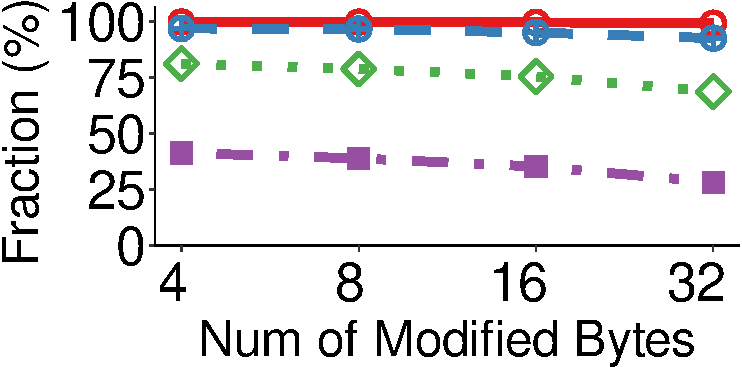
\includegraphics[width=0.45\textwidth]{pic/featurespy/plot/detection/syn/fixed_p_4.pdf} &
        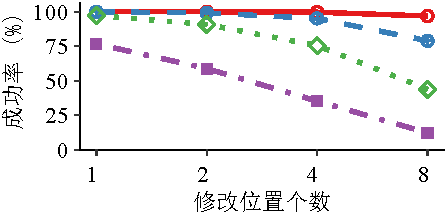
\includegraphics[width=0.45\textwidth]{pic/featurespy/plot/detection/syn/fixed_q_16.pdf}  \\
        \mbox{\small (a) 固定$x=4$,改变$y$}                                                    &
        \mbox{\small (b) 固定$y=16$,改变$x$}                                                     \\
    \end{tabular}
    \caption{(Exp\#1) 明文数据块的相似性检测}
    \label{fig:featurespy-expDetectionSynSim}
\end{figure}

图~\ref{fig:featurespy-expDetectionSynSim}(a)显示了当本文固定$x$=4并变化$y$(图~\ref{fig:featurespy-expDetectionSynSim}(a)),以及固定$y$=16并变化的$x$(图~\ref{fig:featurespy-expDetectionSynSim}(b))时产生的多个SYNChunk$(x, y)$数据集的检测结果。一般来说,识别到相似数据块的成功率随着$x$或$y$的增大而降低,这是因为修改范围越大,越有可能使数据块产生不同的内容特征。具体来说,称功率受$x$的影响比$y$更大,这是因为增加$x$将改变大量滑动窗口(\S\ref{subsec:featurespy-basic})的Rabin指纹。另一方面,本文可以通过检查数据块是否共享任意一个或两个相同的特征来有效地检测大部分(例如,至少78.9\%)的相似数据块。

\paragraph*{Exp\#2(密文数据块的相似性检测)。}
本文扩展Exp\#1来研究\sysnameF 基于密文数据块的的相似性检测能力。实验采用本文提出的相似性保留加密方法(SPE)产生密文数据块。具体来说,本文对每个明文数据块执行特征密钥生成(\S\ref{subsec:featurespy-spe}),检查为每个SYNChunk$(x, y)$中所有数据块生成的密钥相同的比例,以验证相似性保留加密为相似数据块产生相同特征密钥的能力(标记为KeyGen)。然后,本文执行SPE,使用特征密钥加密对应数据块的特征指标,并统计加密后的相似性指标与每个数据集中基本数据块的相似性指标相同的比例作为密文数据块相似性检查能力的结果。这里,本文关注三个SPE实例SPE$(1)$、SPE$(2)$和SPE$(4)$,它们将1个、2个和4个加密块(长度分别为16、32和64个字节)作为每个数据块的相似性指标。

\begin{figure*}[!htb]
    \centering
    
\includegraphics[width=0.4\textwidth]{pic/featurespy/plot/detection/syn/synBarPlotDetect_legend.pdf}\\
    \begin{tabular}{@{}c@{}c}
        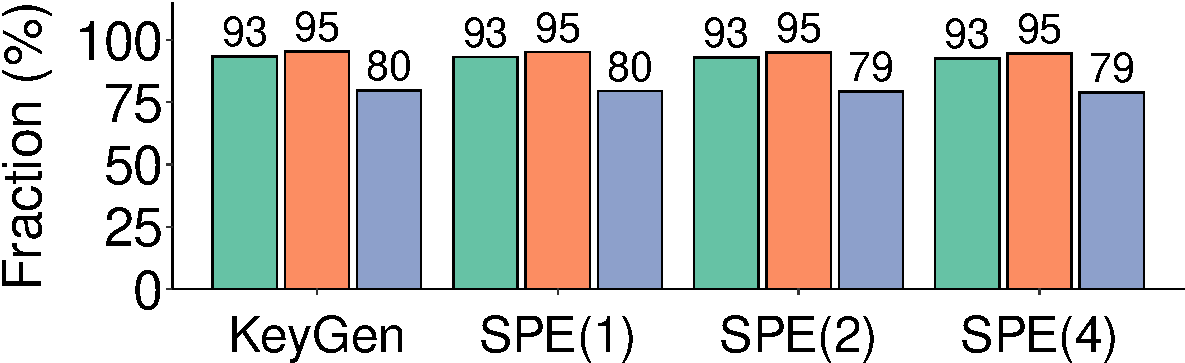
\includegraphics[width=0.49\textwidth]{pic/featurespy/plot/detection/syn/syn-p1-q4-detect.pdf}  &
        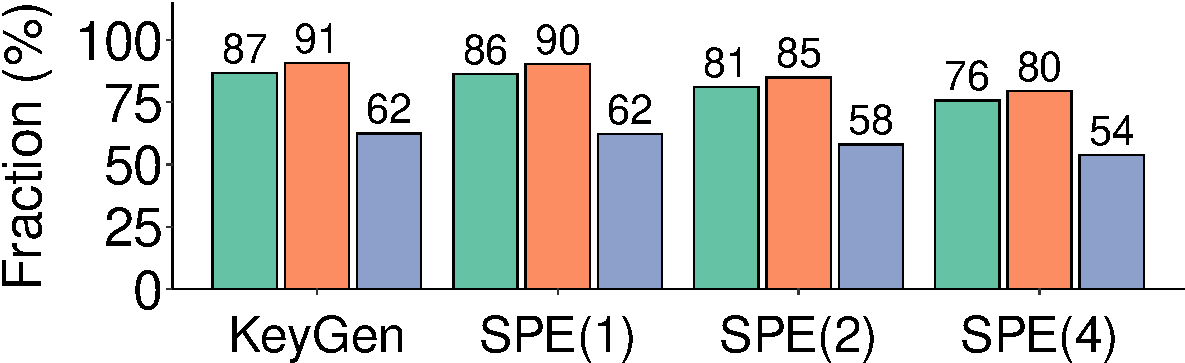
\includegraphics[width=0.49\textwidth]{pic/featurespy/plot/detection/syn/syn-p2-q8-detect.pdf}    \\
        \mbox{\small (a) $\textrm{SYNChunk}(1, 4)$}                                                     &
        \mbox{\small (b) $\textrm{SYNChunk}(2, 8)$}                                                       \\
        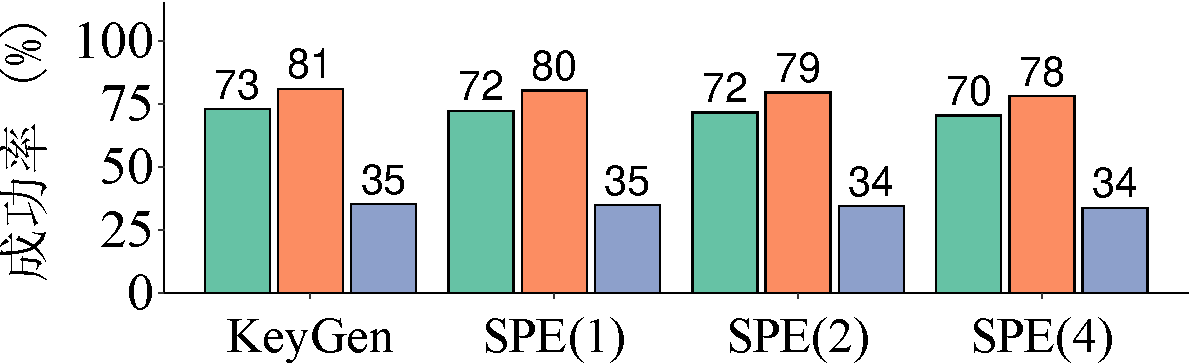
\includegraphics[width=0.49\textwidth]{pic/featurespy/plot/detection/syn/syn-p4-q16-detect.pdf} &
        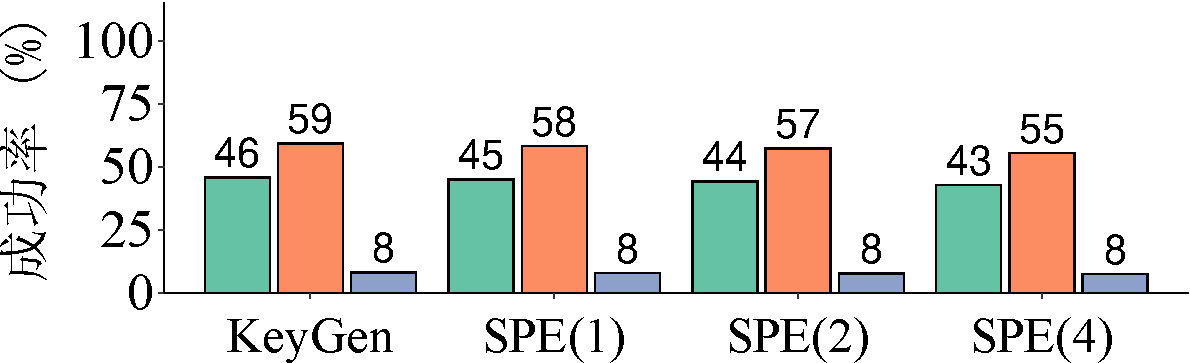
\includegraphics[width=0.49\textwidth]{pic/featurespy/plot/detection/syn/syn-p8-q32-detect.pdf}   \\
        \mbox{\small (c) $\textrm{SYNChunk}(4, 16)$}                                                    &
        \mbox{\small (d) $\textrm{SYNChunk}(8, 32)$}                                                      \\
    \end{tabular}
    \caption{(Exp\#2) 密文数据块的相似性检测}
    \label{fig:featurespy-expDetectionSynDetect}
\end{figure*}

图~\ref{fig:featurespy-expDetectionSynDetect}展示了具有最小(SYNChunk$(1,4)$)、小(SYNChunk$(2,8)$)、中(SYNChunk $(4,16)$)和大(SYNChunk$(8,32)$)差异的相似数据块产生的密文数据块的相似性检查成功率。与\textit{allFeature}相比,实例\textit{firstFeature}和\textit{minFeature}为仅为更相似的数据块生成相同的特征密钥,尤其是当修改量很大时。例如,\textit{firstFeature}和\textit{minFeature}分别为45.7\%和59.3\%的数据块产生相同密钥,但\textit{allFeature}仅为8.1\%的数据块生成了相同特征密钥。此外,\textit{minFeature}为差异较大的相似数据块产生相同特征密钥的能力优于\textit{firstFeature},这可能是因为最小内容特征对数据块内容的随机变化更不敏感。此外,本文观察到相似性保留加密在加密后保留了较高的相似性。具体来说,通过检查密文数据块中的相似性指标,本文在SYNChunk$(1,4)$、SYNChunk$(2,8)$、SYNChunk$(4,16)$和SYNChunk$(8,32)$,分别检测到至多95.2\%、90.4\%、80.2\%和58.3\%的相似数据块。

\paragraph*{Exp\#3(推测内容攻击检测案例研究)。}
本文扩展了\S\ref{sec:featurespy-attack}中的案例研究,以研究 \sysnameF 如何检测推断工资和签约奖金的推测内容攻击。本文用一个固定报告阈值$T$=3\%和一个大小为两个加密块(等效32字节)的相似性指标来配置 \sysnameF。参考\S\ref{sec:featurespy-attack},攻击者需要伪造101$\times$31=3131个文件,其中年薪和签约奖金分别有101和31个可能值。为了模拟在正常数据集中混合伪造文件(否则更容易被检测到)的攻击者,本文将所有伪造文件随机插入到每个Linux/CouchDB(由于FSL和MS数据集不含实际数据,因此不予考虑)快照中的文件之间,并对每个快照中的文件(及伪造的文件)单独执行数据分块\cite{fsl, meyer2011deduplication},并在产生的数据块之上应用相似性保留加密。本文以检测率(\sysnameF 成功检测到的此类攻击快照的数量与使用的快照总数的比率)作为评价标准。此外,本文使用\sysnameF 处理每个原始快照中的所有文件(不包含伪造的文件),评估\sysnameF 的误判率(即\sysnameF 误判的快照数量与原始快照总数的比率)。本文展示了\sysnameF 如何检测推测内容攻击,并给出整体的检测结果。

\begin{figure*}[!htb]
    \centering
    
\includegraphics[width=0.8\textwidth]{pic/featurespy/plot/detection/overall/prefixDistribution_legend.pdf}\\
    \begin{tabular}{cc}
        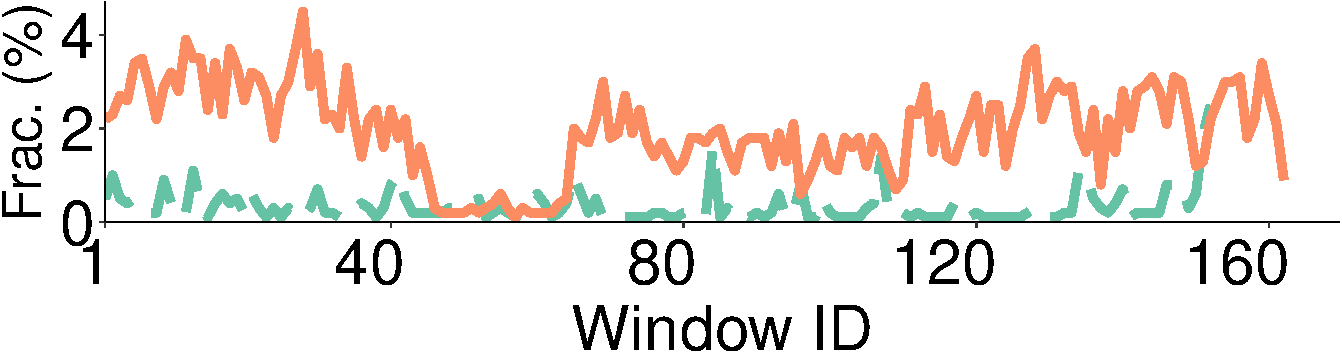
\includegraphics[width=0.472\textwidth]{pic/featurespy/plot/detection/overall/prefixDistribution-1000-Linux-first.pdf} &
        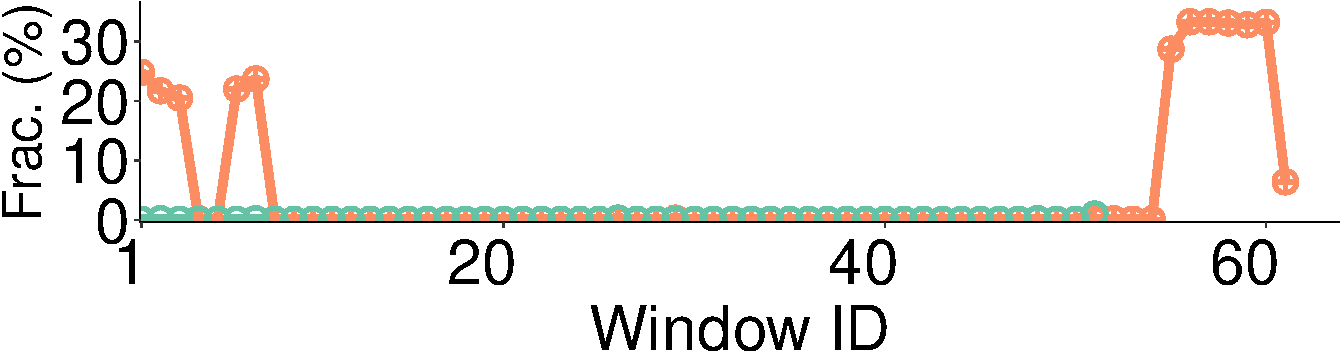
\includegraphics[width=0.472\textwidth]{pic/featurespy/plot/detection/overall/prefixDistribution-1000-CouchDB-first.pdf} \\
        \mbox{\makecell[c]{\small (a) Linux:\textit{firstFeature}实例}}                                                        &
        \mbox{\makecell[c]{\small (b) CouchDB:\textit{firstFeature}实例}}                                                        \\        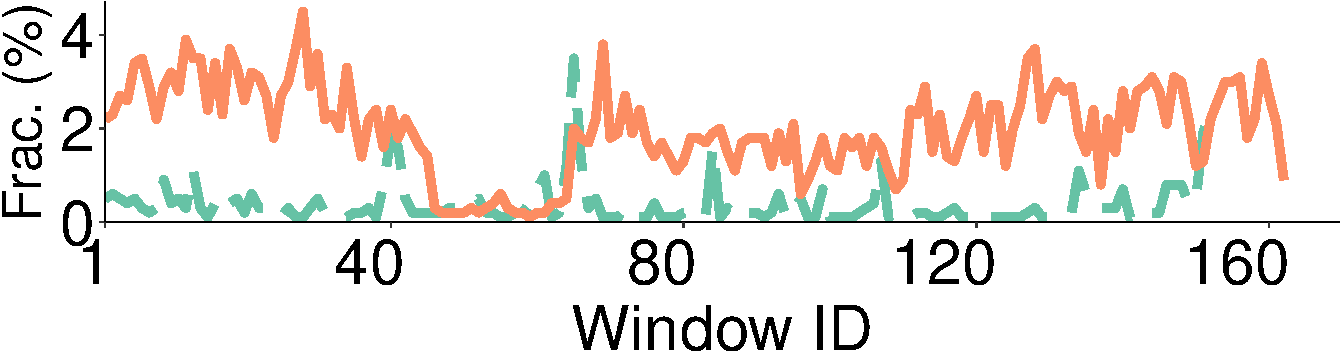
\includegraphics[width=0.472\textwidth]{pic/featurespy/plot/detection/overall/prefixDistribution-1000-Linux-min.pdf} &
        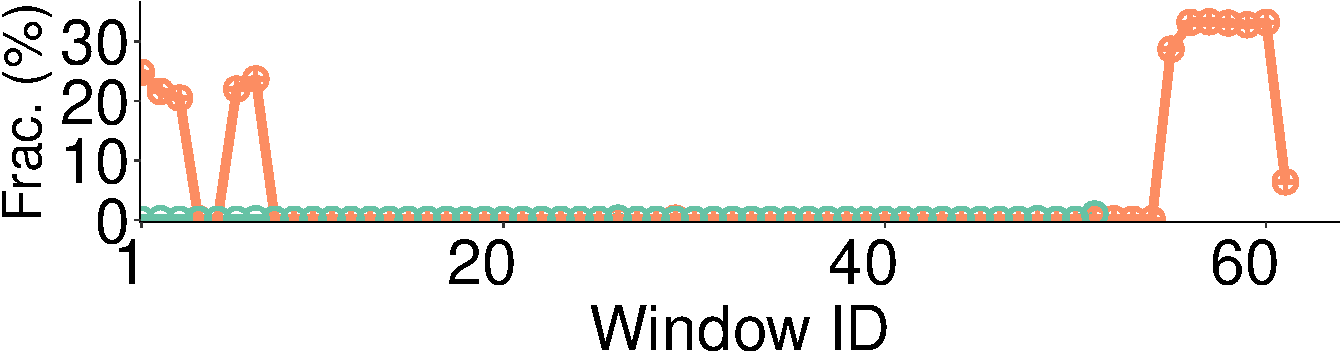
\includegraphics[width=0.472\textwidth]{pic/featurespy/plot/detection/overall/prefixDistribution-1000-CouchDB-min.pdf}   \\
        \mbox{\makecell[c]{\small (c) Linux:\textit{minFeature}实例}}                                                          &
        \mbox{\makecell[c]{\small (d) CouchDB:\textit{minFeature}实例}}                                                          \\
        \includegraphics[width=0.472\textwidth]{pic/featurespy/plot/detection/overall/prefixDistribution-1000-Linux-all.pdf}   &
        \includegraphics[width=0.472\textwidth]{pic/featurespy/plot/detection/overall/prefixDistribution-1000-CouchDB-all.pdf}   \\
        \mbox{\makecell[c]{\small (e) Linux:\textit{allFeature}实例}}                                                          &
        \mbox{\makecell[c]{\small (f) CouchDB:\textit{allFeature}实例}}                                                          \\
    \end{tabular}
    \caption{(Exp\#3)攻击检测示例:给出了使用\textit{firstFeature}、\textit{minFeature}和\textit{allFeature}方案分别处理包含伪造文件(即攻击,Attack)和不包含伪造文件(即不发生攻击,Raw)的Linux/CouchDB最后一个版本的快照时每个窗口(大小固定为$W$=1\,K)中最高频相似性指标的出现频率。}
    \label{fig:featurespy-expDetectionOverall}
\end{figure*}

图~\ref{fig:featurespy-expDetectionOverall}显示了\sysnameF 的三种实例在检测原始Linux快照(v5.13)和CouchDB快照(v6.6.2)以及插入伪造文件后的快照时的结果。具体来说,x轴为处理窗口(大小固定为$W$=1\,K)的顺序编号,y轴为每个窗口中具有相同相似性指标的数据块占该窗口中所有数据块的比例。本文观察到所有三个实例都可以有效地检测到推测内容攻击,因为它们在攻击快照(Attack)中至少有一个窗口的最高频率超过了阈值$T$=3\%(即,具有相同相似性指标的密文数据块的比例大于$T$=3\%)。另一方面,\textit{minFeature}方案在Linux快照中发生了误判,这是由于其至少有一个正常的窗口(例如,Raw的第65个窗口)中,具有相同相似性指标的密文数据块的比例大于阈值$T$=3\%。

\begin{figure}[!htb]
    \centering
    \includegraphics[width=0.5\textwidth]{pic/featurespy/plot/detection/overall/effectiveness-falsePositive_legend.pdf}
    \vspace{5pt}\\
    \begin{tabular}{@{\ }c@{\ }c}
        \includegraphics[width=0.6\textwidth]{pic/featurespy/plot/detection/overall/effectivenessLinux.pdf} &
        \includegraphics[width=0.3\textwidth]{pic/featurespy/plot/detection/overall/falsePositiveLinux.pdf}   \\
        \mbox{\small (a) 检测率}                                                                            &
        \mbox{\small (b) 误判率}                                                                              \\
    \end{tabular}
    \caption{(Exp\#3) 每个Linux/CouchDB快照中的总体检测率和误判率}
    \label{fig:featurespy-expDetectionOverallFalsePositive}
\end{figure}

图~\ref{fig:featurespy-expDetectionOverallFalsePositive}显示了本文将\sysnameF 的检测窗口大小分别配置为1\,K,5\,K和10\,K时Linux数据集中的总体检测率和误判率。在各个窗口大小设置下,\sysnameF 均实现了很高的检测率(例如,至少98.6\%)。然而,较大的窗口会略微降低检测率,这是因为大窗口中仅有相对较小部分的密文数据块具有相同的相似性指标。此外,\sysnameF 仅在窗口大小为1\,K时才会产生误判(图~\ref{fig:featurespy-featureDistribution}(b)),这是因为原始快照(Raw)当中本身包含较多的相似数据块。但即使在这种情况下,\textit{allFeature}也没有任何误判,这是因为它只能检测到少量相似度较高的数据块。另一方面,可检测到更多相似数据块(Exp\#2)的\textit{minFeature}方案会产生28.6\%的误判。

除了Linux数据集,本文也在CouchDB数据集中评估\sysnameF,并发现所有\sysnameF 的实例均可成功检测到所有混合在CouchDB数据集的快照中的推测内容攻击(即具有100\%的检测率),且没有引入任何误判。可能的原因是每个 CouchDB快照中几乎不含有相似数据块,当注入许多对伪造文件产生的相似数据块时,\sysnameF 可以立即检测到(相似数据块的)频率分布变化。

%TODO
\paragraph*{Exp\#4(目标文件熵对攻击检测的影响)。}

本文扩展研究\sysnameF 在检测具有特定信息熵的目标文件时的检测率,即针对具有不同信息熵的目标文件SYNFile$(x, y)$($x$是文件中未知变量的数量,$y$是每个变量的可能取值的数量,参见\S\ref{subsec:featurespy-datasets})的检测能力。本文枚举了目标文件的$x\times y$个可能值,将它们随机插入到Linux数据集最后一个快照(v5.13,大小为985.9\,MiB)包含的文件序列中,并评估100次随机生成的目标文件数据集下\sysnameF 的检测率(阈值设置为固定的$T$=3\%)。

\begin{figure}[!htb]
    \centering
    \includegraphics[width=0.5\textwidth]{pic/featurespy/plot/detection/trade-off/trade_off_legend.pdf}
    \vspace{5pt} \\
    \begin{tabular}{@{\ }c@{\ }c@{\ }c}
        \includegraphics[width=0.32\textwidth]{pic/featurespy/plot/detection/trade-off/varyWindow_linux.pdf}    &
        \includegraphics[width=0.32\textwidth]{pic/featurespy/plot/detection/trade-off/varyModifyPos_linux.pdf} &
        \includegraphics[width=0.32\textwidth]{pic/featurespy/plot/detection/trade-off/varyFileNumber_linux.pdf}  \\
        \makecell[c]{\small (a) 改变窗口大小$W$                                                                   \\ \small 检测SYNFile$(6,2048)$数据集} &
        \makecell[c]{\small (b) 固定窗口大小$W$=5\,K                                                              \\ \small 检测SYNFile$(\cdot,2048)$数据集} &
        \makecell[c]{\small (c) 固定窗口大小$W$=5\,K                                                              \\ \small 检测SYNFile$(6,\cdot)$数据集} \\
    \end{tabular}
    \caption{(Exp\#4)针对不同伪造文件集合的检测率}
    \label{fig:featurespy-expDetectionTradeOff}
\end{figure}

图~\ref{fig:featurespy-expDetectionTradeOff}(a)展示了当改变窗口大小$W$时检测到对SYNFile$(6,2048)$目标文件的攻击的检测率结果。\textit{firstFeature}和\textit{minFeature}的检测率基本不受到窗口大小$W$的影响(例如,始终保持在93\%以上),但\textit{allFeature}的检测率随着窗口大小增大而下降到34\%。其原因是\textit{allFeature}只能检测到少量相似度较高的数据块(Exp\#2),当窗口大小$W$很大时,这些数据块在窗口内的占比很低。图~\ref{fig:featurespy-expDetectionTradeOff}(b)展示了改变目标文件中未知变量$x$的数量时的检测结果。本文观察到,当$x$=9时,\textit{allFeature}的检测率再次急剧下降到21\%,这是因为它无法检测到具有更多差异区域的相似数据块。

图~\ref{fig:featurespy-expDetectionTradeOff}(c)展示了当改变目标文件中每个变量的可能值的数量$y$时的结果。当$y$为512时,所有三个实例的检测率都较低(例如,仅为13\%)。其原因是目标文件的信息熵较低,攻击者只需要构建少量相似的内容,导致\sysnameF 难以在混在的数据块流中找到相似数据块。一种可能的解决方案是配置一个较小的阈值$T$或窗口大小$W$以在检测到少数几个相似数据块时报告攻击行为,但这会增加在不同工作负载中误判的可能性。对此,本文提出了一项未来的研究方向,即如何自动平衡检测对低信息熵文件的攻击和在处理不同工作负载时最大限度地减少误判之间的权衡。
\subsection{系统性能测试}
\label{subsec:featurespy-evaluation-performance}


\paragraph*{Setup.} 本文为性能评估配置了两个测试平台。

\begin{itemize}[leftmargin=*]
\item {\bf LAN.} 它包括三台机器,每台机器配备一个八核 2.9\,GHz Intel Core i7-10700 CPU,一个 4\,TB 7200 RPM Seagate Exos SATA 硬盘驱动器和 32\,GB 内存。所有机器都通过 10\,Gbps 交换机连接,并运行 Ubuntu 20.04.3。

\item {\bf Cloud.} 部署在 {\em 阿里云} \cite{Alibaba}。本文在两个区域租用了几台 {\em ecs.g7t.3xlarge} 虚拟机 (VM) 来分别运行云、关键服务器和多个客户端。同一地域和不同地域的虚拟机分别连接 10\,Gbps 和 100\,Mbps 网络。每个 VM 配备一个 12 核 3.5GHz CPU,由 Intel Xeon (Ice Lake) Platinum 8369B 和 48GiB 内存虚拟化,并安装阿里云 Linux 3.2104。本文另外挂载了以 {\em Alibaba General-Purpose NAS} 作为存储后端的云机。 NAS 可实现高达 15K\,IOPS 的 4\,K 次随机读写,带宽为 150\,MBps。
\end{itemize}

本文进行以下默认配置。对于底层\sysnameF,本文固定$W$ = 5\,K(即大约300\,KiB EPC使用量),$T$ = 3\%,相似性指标的大小为32\,bytes(即,两个块),通过 N-transform提取的特征数量为三个。对于 \prototype,本文配置了三个线程来提取明文数据块的内容特征(除了 Exp\#5,它在单个线程中对 \prototype 的性能进行微基准测试,而 Exp\#6 使用不同的数字来评估 \prototype 的性能用于提取内容特征的线程)和一个 1\,GiB 容器缓存以提高下载性能(\S\ref{sec:featurespy-implementation})。

\subsubsection{Synthetic Workloads}
\label{subsec:featurespy-syn}
本文使用 SYNUnique 评估 \prototype,其中每个 2\,GiB 文件包括全局唯一的块 (\S\ref{subsec:featurespy-datasets})。为了避免磁盘 I/O,本文在每次测试之前将所有数据加载到每个客户端的内存中,并让云端将所有接收到的数据存储在内存中(相对于 Exp\#8 使磁盘 I/O 研究真实云部署) .本文的目标是在不影响重复数据删除和磁盘 I/O 的情况下了解 \prototype 可实现的最大性能,并表明 \prototype 与 SGXDedup \cite{ren21} 相比会产生有限的性能开销。本文将每个实验的结果平均超过 10 次,并将 {\em Student's t-Distribution} 的 95\% 置信区间包含在条形图中(为简洁起见,本文将它们从折线图中排除)。

\paragraph*{Exp\#5(微基准测试)。}
本文从微基准评估开始,在 LAN 测试平台的不同机器上部署客户端、关键服务器和云。本文让客户端在 SYNUnique 中两次上传相同的 2\,GiB 文件,并在单个线程中评估不同上传步骤的处理时间。考虑的步骤包括: (i) {\em chunking},将输入文件划分为可变大小的明文数据块; (ii) {\em 特征生成},提取每个明文数据块的内容特征,并根据 \sysnameF 实例对目标特征进行采样; (iii) {\em 指纹},计算每个明文数据块的指纹; (iv) {\em key generation},生成特征密钥和 MLE 密钥; (v) {\em encryption},对每个明文数据块进行加密; (vi) {\em detection},基于密文数据块检测推测内容攻击; (vii) {PoW},证明每个密文数据块的所有权; (viii) {\em deduplication},云检测重复块; (ix) {\em transfer},它传输不重复的密文数据块和文件元数据。



\begin{table}[t]
    \small
    \centering
    \setlength{\tabcolsep}{5pt}
    \renewcommand{\arraystretch}{1.05}
    \setlength{\tabcolsep}{0.006\textwidth}{
    \begin{tabular}{|c|c|c|c|c|}
        \hline
        \multicolumn{2}{|@{\,}c|}{\textbf{Procedure/Step}} & \multicolumn{1}{l|}{\hspace{.5em}\textbf{firstFeature}} &
        \multicolumn{1}{c|}{\textbf{minFeature}} &
        \multicolumn{1}{c|}{\textbf{allFeature}} \\ \hline \hline
        \multicolumn{2}{|c|}{Chunking} & \multicolumn{3}{c|}{$2.12\pm0.006$} \\ \hline
        \multicolumn{2}{|c|}{\makecell[c]{Feature generation}} &
        \makecell[c]{$4.34 \pm 0.01$} & \makecell[c]{$9.93 \pm0.04$} & \makecell[c]{$9.85 \pm0.02$} \\ \hline
        \multicolumn{2}{|c|}{\makecell[c]{Fingerprinting}}&
        \multicolumn{3}{c|}{$1.81 \pm 0.002$} \\ \hline        \multicolumn{2}{|c|}{\makecell[c]{Key generation}}&
        \multicolumn{3}{c|}{$0.73 \pm 0.02$ ($0.49 \pm 0.01$)} \\ \hline
        \multicolumn{2}{|c|}{Encryption} & \multicolumn{3}{c|}{$1.22 \pm 0.001$} \\ \hline
        \multirow{2}{*}{In Enclave}
        & Detection &
        \multicolumn{3}{c|}{$0.04   \pm 0.005$} \\ \cline{2-5}
        & PoW &
        \multicolumn{3}{c|}{$1.86   \pm 0.004$} \\ \hline
        \multicolumn{2}{|c|}{Deduplication}  &
        \multicolumn{3}{c|}{$0.55 \pm 0.02$}  \\ \hline
        \multicolumn{2}{|c|}{Transfer}  & \multicolumn{3}{c|}{$1.16 \pm 0.03$ ($0.04 \pm 0.001$)}\\ \hline
    \end{tabular}
    }
    \caption{(Exp\#5) 处理随机文件数据每 1\,MiB 的时间分解(单位:ms)。 除括号中明确指定外,第二次上传的每一步所消耗的时间与第一次上传的相同。}
    \label{tab:featurespy-evaluation-syn-system-breakdown}
    \vspace{-6pt}
\end{table}
表~\ref{tab:featurespy-evaluation-syn-system-breakdown} 展示了结果(每 1\,MiB 文件数据处理)。由于 \prototype 建立在 SGXDedup \cite{ren21} 之上,它继承了在第二次上传中卸载密钥生成 (\S\ref{sec:featurespy-implementation}) 的计算开销以及避免传输重复块的性能优势.检测步骤是高效的,并且在上传过程中占用了总时间的 0.4\%。此外,由于 N-transform的计算开销,特征生成步骤很昂贵。例如,{\tt firstFeature} 在第一次上传时占用了总时间的 31.4\%; {\tt minFeature} 和 {\tt allFeature} 所消耗的时间分数分别进一步增加到 51.1\% 和 50.9\%,因为它们提取了所有三个特征(与只提取第一个特征的 {\tt firstFeature} 相反) )。然而,本文认为本文可以通过多线程来减轻特征生成的性能开销(见下文)。


\paragraph*{Exp\#6(单客户端性能)。}
本文考虑单个客户端,并将 \prototype 的性能与基本系统 SGXDedup 进行比较。本文让客户端两次上传相同的文件(如 Exp\#5)并进一步下载文件。


图~\ref{fig:featurespy-singleClientThroughput}(a) 和Figure~\ref{fig:featurespy-singleClientThroughput}(b) 分别展示了当本文改变提取特征的线程数(\S\ref{sec:featurespy-implementation})。 SGXDedup 的速度在第一次上传时保持为 297.1\,MiB/s,在第二次上传时保持为 304.3\,MiB/s,因为它不提取特征。 \prototype 的上传速度首先随着线程数的增加而增加(例如,{\tt firstFeature} 为 265.3\,MiB/s,{\tt minFeature} 为 261.3\,MiB/s,{\tt minFeature} 为 262.6\,MiB/s {\tt allFeature} 当三个线程用于在第一次上传中提取特征时),然后减少(例如,在第一次上传中大约为 220\,MiB/s 和在第二次上传中为 225\,MiB/s 对于所有三个实例)由于资源争用。通过利用多线程,\prototype 仅在第一次上传时比 SGXDedup 产生 8.0-12.0\% 的性能开销,在第二次上传时为 6.6-7.5\%。此外,本文观察到第一次和第二次(不需要传输重复数据)上传之间的性能差异很小,因为本文的 LAN 测试平台具有高带宽来传输数据。本文认为源端重复数据删除在实际云部署中带来了显着的性能提升(Exp\#8),并减少了处理实际存储工作负载的网络流量(Exp\#10)。图~\ref{fig:featurespy-singleClientThroughput}(c)比较下载速度。 \prototype 会导致 1.3\% 的性能下降,因为它使用 MLE 密钥和特征密钥解密每个块。


\begin{figure}[t]
    \centering
    \includegraphics[width=0.7\textwidth]{pic/featurespy/plot/performance/LANSyn/legend.pdf}\\
    \vspace{1pt}
    \begin{tabular}{@{\ }c@{\ }c@{\ }c}
        \includegraphics[width=0.32\textwidth]{pic/featurespy/plot/performance/LANSyn/upload_thread_line.pdf}&
        \includegraphics[width=0.32\textwidth]{pic/featurespy/plot/performance/LANSyn/upload_thread_2nd_line.pdf}&
        \includegraphics[width=0.32\textwidth]{pic/featurespy/plot/performance/LANSyn/download_bar.pdf}\\
        \makecell[c]{\small (a) 1st upload} &
        \makecell[c]{\small (b) 2nd upload} &
        \makecell[c]{\small (c) Download}\\
    \end{tabular}
    \vspace{-6pt}
    \caption{(Exp\#6) LAN 测试平台中的单客户端性能。 在下载中,所有 \prototype 实例都达到相同的速度,本文将它们(橙色)与 SGXDedup(绿色)进行比较。}
    \vspace{-6pt}
    \label{fig:featurespy-singleClientThroughput}
\end{figure}

\paragraph*{Exp\#7(多客户端性能)。}
本文评估多个客户端同时发出上传/下载时的性能。 本文使用云测试台来考虑越来越多的客户端,并将所有客户端、关键服务器和云部署在同一个区域。 本文将 {\em 聚合上传(下载)速度}衡量为总上传(下载)数据大小与所有客户端完成上传(下载)总时间的比率。

\begin{figure}[t]
    \centering
    \includegraphics[width=0.7\linewidth]{pic/featurespy/plot/performance/multiClient/legend.pdf}\\
    \vspace{1pt}
    \begin{tabular}{@{\ }c@{\ }c@{\ }c}
            \includegraphics[width=0.32\textwidth]{pic/featurespy/plot/performance/multiClient/upload_1st_line.pdf}&
            \includegraphics[width=0.32\textwidth]{pic/featurespy/plot/performance/multiClient/upload_2nd_line.pdf}&
            \includegraphics[width=0.32\textwidth]{pic/featurespy/plot/performance/multiClient/download_line.pdf}\\
            \makecell[c]{\small (a) 1st upload} &
            \makecell[c]{\small (b) 2nd upload} &
            \makecell[c]{\small (c) Download}\\
        \end{tabular}
        \vspace{-11pt}
        \captionof{figure}{(Exp\#8) 多客户端性能。 所有 \prototype 实例的下载速度都是相同的,本文将它(橙色)与 SGXDedup(绿色)进行比较。}
        \vspace{-5pt}
        \label{fig:featurespy-expMultiClientThroughput}
\end{figure}

\begin{table}[t]
               \centering
                 \small
          \begin{tabular}{|c|c|c|c|}
                \hline
                {\bf Approach} & {\bf 1st Upload} & {\bf 2nd Upload} & {\bf Download} \\
                \hline
                \hline
                Transfer & \multicolumn{3}{c|}{11.8 $\pm$ 0.04} \\
                \hline
                \hline
                \makecell[c]{\tt firstFeature} & \multirow{3}{*}{11.5 $\pm$ 0.006} & 204.4 $\pm$ 10.06 & \multirow{3}{*}{11.5 $\pm$ 0.004} \\
                \cline{1-1}\cline{3-3}
                \makecell[c]{\tt minFeature} &  & 184.7$\pm$ 7.4 &  \\
                \cline{1-1}\cline{3-3}
                \makecell[c]{\tt allFeature} &  & 185.0$\pm$ 6.4 &  \\
                \hline
                SGXDedup & 11.5 $\pm$ 0.009 & 233.2 $\pm$ 8.4 & 11.5 $\pm$ 0.004 \\
                \hline
            \end{tabular}
        \vspace{2pt}
        \captionof{table}{(Exp\#7) 实云部署(单位:MiB/s)。 本文使用 {\tt scp} 将 2\,GiB 文件从客户端上传到云端,以提供环境中的传输基准。}
        \label{tab:featurespy-expCloudTest}
\end{table}

图~\ref{fig:featurespy-expMultiClientThroughput} 最多显示 10 个客户端的结果。本文不考虑更多的客户端,因为总体上传速度已经基本稳定。具体来说,第一次和第二次上传的速度都随着客户端数量的增加而增加,然后由于云端的写入竞争而逐渐降低。本文观察到 SGXDedup 比 \prototype 更早达到峰值性能(例如,四个客户端在第一次上传时达到 924.9\,MiB/s)(例如,在第一次上传中,六个客户端达到 882.2\,MiB/s),因为它实现了高性能并且云很容易饱和。类似地,由于读取云中的争用。


\paragraph*{Exp\#8(实云部署)。}
本文扩展 Exp\#6 来研究云测试平台中的单客户端性能。本文将客户端和密钥服务器部署在同一地域的两台虚拟机中,以及不同地域的云中(相对于Exp\#7,所有实体都部署在同一地域),从而模拟场景Internet 连接在客户端和云之间。此外,本文让客户端从本地磁盘(即,读写速度约为 270\,MiB/s 用于读取/写入的 SSD)读取文件进行上传,云存储接收到的数据在附加的 NAS 中。本文使用 {\tt scp} 来对客户端和云之间的传输速度进行基准测试。


表~\ref{tab:featurespy-expCloudTest} 显示了结果。在第一次上传中,所有方法的性能都受到传输速度的限制。在第二次上传中,SGXDedup 和 {\tt firstFeature} 的性能受到分块(Table~\ref{tab:featurespy-evaluation-syn-system-breakdown})的限制,而 {\tt firstFeature} 产生 12.3\% 的性能开销SGXDedup,因为它额外提取了第一个特征来生成密钥。 {\tt minFeature} 和 {\tt allFeature}(在第二次上传中)的性能受特征提取的限制。请注意,所有方法的第二次上传速度都比 LAN 测试平台中的(Exp\#6)慢,原因有三个。首先,本文现在处理磁盘文件并启用磁盘 I/O。此外,云测试平台中的虚拟机是从物理机虚拟化的,在处理计算密集型操作时可能会导致性能下降。
此外,互联网的高延迟减慢了重复数据删除中指纹的传输速度。
在下载中,所有方法的性能都受到传输速度的限制,与 SGXDedup 相比,\prototype 会产生 0.6\% 的开销。


\subsubsection{实际工作负载}
\label{subsec:featurespy-real}
本文使用 FSL 和 MS 评估 \prototype,以了解其在处理真实世界大规模数据时的性能。

\paragraph*{Exp\#9(跟踪驱动的性能)。}
本文评估了 LAN 测试平台中的上传和下载性能。本文从 FSL 和 MS 中分别选择了 10 个快照,如下所示。对于 FSL,本文选择来自同一用户的每周快照以具有高交叉快照冗余;对于 MS,本文选择具有最多快照内冗余的快照。选择的 FSL 和 MS 快照分别采用 407.5\,GiB 和 902.5\,GiB 的预重复数据删除数据。由于本文的快照只包含块指纹和大小(\S\ref{subsec:featurespy-datasets}),本文通过重复将其指纹写入具有相应指定大小的备用块来重建每个明文数据块。本文先一张一张上传快照,然后按照上传的顺序下载。注意原来的 SGXDedup \cite{ren21} 没有容器缓存(\S\ref{sec:featurespy-implementation});为了公平比较,本文为 SGXDedup 实现了一个内存缓存来缓冲最近恢复的容器,并将其配置为与 \prototype 相同的大小 (1\,GiB)。


\begin{figure}[t]
    \centering
    \includegraphics[height=0.2in]{pic/featurespy/plot/performance/LANTrace/trace_legend_upload.pdf}\\
    \includegraphics[height=0.2in]{pic/featurespy/plot/performance/LANTrace/trace_legend_download.pdf}\\
    \vspace{3pt}
    \begin{tabular}{@{\ }c@{\ }c}
        \includegraphics[width=0.47\textwidth]{pic/featurespy/plot/performance/LANTrace/trace_fsl.pdf}&
        \includegraphics[width=0.47\textwidth]{pic/featurespy/plot/performance/LANTrace/trace_ms.pdf}\\
        \mbox{\small (a) FSL} &
        \mbox{\small (b) MS}\\
        \includegraphics[width=0.47\textwidth]{pic/featurespy/plot/performance/LANTrace/trace_linux.pdf}&
        \includegraphics[width=0.47\textwidth]{pic/featurespy/plot/performance/LANTrace/trace_couch.pdf}\\
        \mbox{\small (c) Linux} &
        \mbox{\small (d) CouchDB}\\
    \end{tabular}
    \vspace{-6pt}
    \caption{(Exp\#9) Trace-driven performance.}
    \vspace{-6pt}
    \label{fig:featurespy-traceDrivenThroughput}
\end{figure}
图~\ref{fig:featurespy-traceDrivenThroughput} 展示了结果。在第一个 FSL 快照之后(例如,224.8\,MiB/s, 223.9\,MiB/s, 214.9\,MiB/s 和 216.9\,MiB/s 用于 SGXDedup、{\tt firstFeature}、{\tt minFeature} 和{\tt allFeature}),SGXDedup 和 \prototype 都实现了高性能(例如,至少 298.9\,MiB/s, 266.8\,MiB/s, 246.4\,MiB/s 和 248.8\,MiB/s SGXDedup、{\tt firstFeature}、{\tt minFeature} 和 {\tt allFeature}),因为它们不需要传输在 FSL 中占很大比例的交叉快照冗余。下载速度通常是稳定的(例如 SGXDedup 为 88.7-102.6\,MiB/s,\prototype 为 88.0-100.2\,MiB/s)。平均而言,与 SGXDedup 相比,{\tt firstFeature}、{\tt minFeature} 和 {\tt allFeature} 分别降低了上传性能 8.8\%、15.7\% 和 15.0\%,下载性能降低了 0.8 \%。

与 FSL 相比,MS 中的上传性能通常下降约 21\%,因为 MS 包含许多独特的块并导致较大的指纹索引(通过 LevelDB \cite{leveldb} 实现)。这加重了查询指纹索引是否存在密文数据块以进行重复数据删除的开销。此外,MS 中的下载速度会随着快照的变化而波动,因为一些快照具有更多的非重复块,并且可能存储在可以通过顺序读取快速访问的连续区域(即碎片较少的 \cite{lillibridge13})中。


\paragraph*{Exp\#10(网络流量分析)。}
本文分析了 \prototype 的网络流量,并将其与三种可以抵御推测内容攻击的重复数据删除方法进行比较:(i) {\em target-based deduplication} \cite{harnik2010side},强制客户端传输所有密文数据块到云端; (ii) {\em random-threshold deduplication} \cite{harnik2010side},如果每个块的上传次数小于预定义的阈值,则执行基于存储目标的重复数据删除,或源端重复数据删除 (\S\ref{sec:background-enc-deduplication}) 否则; (iii) {\em 两阶段重复数据删除} \cite{li15},它对来自同一客户端的密文数据块执行源端重复数据删除,然后对跨不同客户端的密文数据块执行基于存储目标的重复数据删除。在这里,本文按照之前的工作 \cite{harnik2010side} 分别在 20 和 2 处选择随机阈值重复数据删除中阈值的上限和下限。本文专注于 FSL 和 MS。对于 FSL,本文每天合并每个用户的快照,并按时间顺序存储。对于 MS,本文认为每个快照都来自一个单独的客户端,并按照快照 ID 的顺序存储快照。本文不考虑文件元数据导致的带宽开销。

\begin{figure}[t]
    \centering
    \includegraphics[width=0.8\textwidth]{pic/featurespy/plot/bandwidth/upload_traffic_legend.pdf}     \vspace{3pt} \\
    \begin{tabular}{@{\ }c@{\ }c}
        \includegraphics[width=0.47\textwidth]{pic/featurespy/plot/bandwidth/upload_traffic_fsl.pdf} &
        \includegraphics[width=0.47\textwidth]{pic/featurespy/plot/bandwidth/upload_traffic_ms.pdf} \\
        {\small (a) FSL} & {\small (b) MS} \\
        \includegraphics[width=0.47\textwidth]{pic/featurespy/plot/bandwidth/upload_traffic_linux.pdf} &
        \includegraphics[width=0.47\textwidth]{pic/featurespy/plot/bandwidth/upload_traffic_couch.pdf} \\
        {\small (c) Linux} & {\small (d) CouchDB}
    \end{tabular}
    \vspace{-6pt}
    \caption{(Exp\#10) 存储每个快照后的累积网络流量。}
    \vspace{-6pt}
    \label{fig:featurespy-expNetworkTraffic}
\end{figure}

图~\ref{fig:featurespy-expNetworkTraffic} 展示了结果。由于 \prototype 执行纯源端重复数据删除,因此它优于其他方法。例如,在存储最后一个快照后,\prototype 将基于存储目标的重复数据删除的网络流量在 FSL 中减少了 98.9\%,在 MS 中减少了 83.1\%。两阶段重复数据删除在 ​​FSL 中表现良好(例如,只有 3.7\% 的带宽开销超过 \prototype),因为 FSL 包含大量用户内冗余。但是,在 MS 中,两级重复数据删除的网络流量最终是 \prototype 的 3.1$\times$。随机阈值重复数据删除会在 FSL(例如,\prototype 的 72.5$\times$)和 MS(例如,\prototype 的 2.6$\times$)中产生不同的网络流量。

由于 Linux 和 CouchDB 数据集的每个版本几乎没有冗余,并且需要大量源端重复数据删除查询,对于 Linux,它仅带来 $1.05\%$ 的流量节省,而对于 CouchDB,它甚至导致 $0.31 \%$ 额外的流量开销。随机阈值重复数据删除带来的流量节省是完全不同的。在 MS 中,它带来了 $55.75\%$ 的流量节省,而在 FSL 和 Linux 中,只有 $21.60\%$ 和 $26.68\%$。然而,它甚至在 CouchDB 中引入了 $0.0016\%$ 的额外流量开销。另外,本文发现在CouchDB的前35个版本中,几个方案的网络流量几乎是一样的,而对于后面的版本,\prototype 的累计网络流量几乎保持在一个水平。这是因为这 35 个版本是通用版本,几乎没有冗余。并且这些通用版本和社区/企业版本之间存在大量冗余,使得\prototype 不再需要上传大量数据。
\section{相关研究}
\label{sec:related-work}

\paragraph{安全重复数据删除方法。}
在 \S\ref{sub:basics} 中,我们回顾了针对重复数据删除的两个正交威胁。 MLE (及其变体 \cite{bellare13a, bellare13b, douceur02, li15}) 保护数据机密性以防止受损云,并从安全理论 \cite{bellare15, abadi13} 进行了广泛研究,并在存储系统 \cite{cox02, adya02, bellare13b, armknecht15, shah15, li15, li19, qin17, li20a, ren21}。 \sysnameF 提出了 SPE (\S\ref{sub:spe}),它通过相似性保留来增强 MLE,从而检测基于密文块的学习内容攻击。


PoW 可防止恶意客户端在基于数据源的重复数据删除中损害数据所有权,但无法解决学习内容攻击 (\S\ref{sub:attack})。 \sysnameF 通过主动检测学习内容攻击来补充加密重复数据删除 \cite{ren21}。虽然以前的研究可以通过以不同的方式应用重复数据删除来击败学习内容攻击,但它们会注入网络流量来传输重复的内容。 \sysnameF 执行纯基于数据源的重复数据删除并实现带宽效率 (Exp\#10)。


\paragraph{基于 SGX 的安全应用程序。}
SGX 已被广泛用于加强不同应用系统的安全性,例如比特币\cite{matetic19}、文件系统\cite{ahmad18、shinde20}、外包数据库\cite{eskandarian17、priebe18、sun21}、键值存储\ cite{mishra18, bailleu19, kim19, bailleu21} 和数据分析平台 \cite{schuster15, zheng17, bowe20}。本文重点介绍重复数据删除存储系统。 S2Dedup \cite{miranda21} 管理一个云端安全区来执行安全的重复数据删除,但它依赖于客户端完全受信任的假设。本文扩展了 SGXDedup \cite{ren21} 以防止恶意客户端发起学习内容攻击。
\section{本章小结}
\label{sec:featurespy-conclusion}
本文解决了加密后重复数据删除中的学习内容攻击。 我们提出了 \sysnameF,它通过主动检测客户端 TEE 中的学习内容攻击来增强加密后重复数据删除。 它基于恶意客户端枚举许多相似数据进行攻击的洞察力,并通过检测处理内容中的相似块来报告攻击。 此外,本文提出了 SPE,并允许直接对密文块进行检测。 评估表明,\sysnameF 不仅有效地检测到学习内容攻击,而且在 SGXDedup \cite{ren21} 中部署时会产生有限的性能开销。

\chapter{全文总结与展望}

\section{全文总结}

本文以可信执行环境在加密后重复数据删除中的应用为研究背景,主要对提升服务器辅助消息锁加密

本文基于可信执行环境(TEE)解决了加密后重复数据删除中的性能问题。本文提出了\sysnameS,它实现了一组安全区内部调用以在安全区内执行敏感操作,从而在保持安全性的同时加速加密重复数据删除。\sysnameS 包含三项关键设计:(1)安全高效的安全区管理;(2)自更新的会话密钥管理;以及(3)用于减轻在线加解密开销的基于TEE的推测性加密。此外,本文的实验分析表明\sysnameS 在合成数据集和真实世界数据集作为工作负载的情况下具有远超现有基于密码学机制的加密重复数据删除的性能表现。

本章解决了加密后重复数据删除中的推测内容攻击,提出了\sysnameF,它通过在客户端TEE中主动检测推测内容攻击来增强加密后重复数据删除。它建立在以下观察的基础之上:发起推测内容攻击的而已客户端往往会枚举大量相似的伪造文件进行攻击。因此,可通过检测较小时间段内处理数据中相似数据块出现频率来检测推测内容攻击。此外,本文提出了特征保留加密技术(SPE),并实现了基于密文的数据块相似性检查。实验分析表明\sysnameF 不仅可以有效的检测推测内容攻击,且在\sysnameS 中部署时仅产生有限的额外性能开销。


\section{后续工作展望}

高性能加密后重复数据删除及可信执行环境在存储系统中的应用等相关研究近几年发展迅速,在本文研究工作的基础上,仍有以下方向值得进一步研究:


\thesisacknowledgement
在攻读硕士研究生学历期间,首先衷心感谢我的恩师李经纬对我的淳淳教诲和悉心关怀,在我本科和硕士学习期间,他给予了我生活上、学习上无微不至的关心。恩师对我的指导和影响之大,怎样言说都表达不尽,自己取得的点滴成绩无不凝聚着恩师的心血。恩师国际化的视野,前沿而精髓的学术造诣,严谨勤奋的治学风格,都让我永志不忘,深刻影响着我日后的工作和生活。

衷心感谢张小松教授和网络空间安全研究院为我提供的高水平研究平台以及方方面面的帮助和支持。由衷感谢各位同学朋友们,感谢我们一起度过的或艰难或开心的岁月。

衷心感谢我的父母、家人们,在我的求学生涯中不断的支持我,关心我,鼓励我。其中,我要特别感谢我最最最可爱最最最优秀的小仙女罗楠,在生活中始终像小太阳一般照耀着我,温暖着一切。未来的路还很长,相信我们可以将所有走过的荆棘都化为铠甲,所有可能会到来的风雨也能够泰然处之。

最后,感谢伟大的中国共产党,在百年间矢志践行初心使命、筚路蓝缕奠基立业、创造辉煌开辟未来,建设出美丽富饶、朝气蓬勃的新中国!

\thesisappendix
\section*{实验6中的部分原始数据}
下表为FSL数据集中User004在基于分布的攻击中按文件类型区分的的实验数据。
\begin{table}[!htbp]
\centering
\caption{基于分布的攻击(安全隐患分析)对FSL数据集User4的实际攻击结果}
\label{tab:exp6-user4}
\begin{tabular}{@{}ccccccc@{}}
\toprule
 文件类型 & 正确块数 & 总块数   & 正确唯一块数 & 总唯一块数 & \tabincell{c}{正确块占比\\超10\%的文件} & 文件总数 \\ \midrule
doc  & 1      & 192     & 1       & 108    & 0               & 24   \\
docx & 0      & 30      & 0       & 22     & 0               & 14   \\
pptx & 355    & 19184   & 330     & 9484   & 0               & 38   \\
jpg  & 7      & 484     & 7       & 434    & 1               & 384  \\
png  & 0      & 1284    & 0       & 722    & 0               & 160  \\
img  & 0      & 4       & 0       & 4      & 0               & 4    \\
amr  & 0      & 10976   & 0       & 5496   & 0               & 16   \\
c    & 1896   & 11290   & 1896    & 9826   & 1579            & 8362 \\
h    & 70     & 816     & 70      & 770    & 69              & 724  \\
py   & 2      & 60      & 2       & 53     & 2               & 46   \\
js   & 0      & 24      & 0       & 17     & 0               & 10   \\
data & 0      & 108     & 0       & 86     & 0               & 64   \\
db   & 33     & 5300    & 27      & 2660   & 9               & 58   \\
json & 0      & 346     & 0       & 194    & 0               & 42   \\
po   & 0      & 2616    & 0       & 1333   & 0               & 50   \\
xml  & 151    & 888     & 151     & 841    & 145             & 794  \\
pb   & 0      & 160     & 0       & 159    & 0               & 158  \\
gz   & 4      & 24474   & 4       & 12274  & 4               & 74   \\
bz2  & 0      & 1028    & 0       & 570    & 0               & 112  \\ 
html & 1      & 112     & 1       & 103    & 1               & 94   \\
log  & 8      & 1486    & 8       & 1206   & 8               & 926  \\
sh   & 453    & 2614    & 453     & 2274   & 381             & 1934 \\
out  & 2122   & 84548   & 860     & 37431  & 49              & 2716 \\
txt  & 226    & 1268    & 226     & 1089   & 181             & 910  \\
vmdk & 307356 & 1657924 & 213180  & 640077 & 22              & 48   \\
\bottomrule
\end{tabular}
\end{table}


\thesisbibliography{reference}

\begin{thesistheaccomplish}
    \section{学术论文}
    \bibitem{SGXDedup} \textbf{Ren, Yanjing} and Li, Jingwei and Yang, Zuoru and Lee, Patrick PC and Zhang, Xiaosong. Accelerating Encrypted Deduplication via SGX[C]. Proc.of USENIX ATC, 2021, 957-971. \textbf{CCF-A}
    \bibitem{TED} Li, Jingwei and Yang, Zuoru and \textbf{Ren, Yanjing} and Lee, Patrick PC and Zhang, Xiaosong. Balancing storage efficiency and data confidentiality with tunable encrypted deduplication[C]. Proc. of EuroSys, 2020, 1-15. \textbf{CCF-B}
    \bibitem{Metadedup} Li, Jingwei and Lee, Patrick PC and \textbf{Ren, Yanjing} and Zhang, Xiaosong. Metadedup: Deduplicating metadata in encrypted deduplication via indirection[C]. Proc. of MSST, 2019, 269-281. \textbf{CCF-B}
    \bibitem{TEDExt} Yang, Zuoru and Li, Jingwei and \textbf{Ren, Yanjing} and Lee, Patrick PC and Zhang, Xiaosong. Tunable Encrypted Deduplication with Attack Resilient Key Management[J]. ACM Transactions on Storage (TOS), 2022. \textbf{CCF-A}
    \bibitem{MetadedupExt} Li, Jingwei and Huang, Suyu and \textbf{Ren, Yanjing} and Yang, Zuoru and Lee, Patrick PC and Zhang, Xiao-song and Hao, Yao. Enabling Secure and Space Efficient Metadata Management in Encrypted Deduplication[J]. IEEE Transactions on Computers (TC), 2021. \textbf{CCF-A}
    \bibitem{Attack} Li, Jingwei and Wei, Guoli and Liang, Jiacheng and \textbf{Ren, Yanjing} and Lee, Patrick PC and Zhang, Xiaosong. Revisiting Frequency Analysis against Encrypted Deduplication via Statistical Distribution[C]. Proc. of IEEE INFOCOM, 2021. \textbf{CCF-A}
    \section{发明专利}
    \bibitem{CN111338572B} 李经纬, 杨祚儒, \textbf{任彦璟}, 李柏晴, 张小松. 一种可调节加密重复数据删除方法:CN111338572B[P]. 2021-09-14.
    \bibitem{CN110109617B} 李经纬, 李柏晴, \textbf{任彦璟}, 张小松. 一种加密重复数据删除系统中的高效元数据管理方法:CN110109617B[P]. 2020-05-12.
    \bibitem{CN112947855A} 李经纬, \textbf{任彦璟}, 杨祚儒, 李柏晴, 张小松. 一种基于硬件安全区的高效加密重复数据删除方法:CN112947855A[P]. 2021-06-11.
    \bibitem{CN112152798A} 李经纬, 黄苏豫, \textbf{任彦璟}, 杨祚儒, 李柏晴. 基于加密数据去重的分布式密文共享密钥管理方法及系统:CN112152798A[P]. 2020-12-29.
\end{thesistheaccomplish}

% \thesistranslationoriginal
% \section{}

% \thesistranslationchinese
% \section{}

\end{document}